% Options for packages loaded elsewhere
\PassOptionsToPackage{unicode}{hyperref}
\PassOptionsToPackage{hyphens}{url}
%
\documentclass[
  english,
  man]{apa6}
\usepackage{lmodern}
\usepackage{amssymb,amsmath}
\usepackage{ifxetex,ifluatex}
\ifnum 0\ifxetex 1\fi\ifluatex 1\fi=0 % if pdftex
  \usepackage[T1]{fontenc}
  \usepackage[utf8]{inputenc}
  \usepackage{textcomp} % provide euro and other symbols
\else % if luatex or xetex
  \usepackage{unicode-math}
  \defaultfontfeatures{Scale=MatchLowercase}
  \defaultfontfeatures[\rmfamily]{Ligatures=TeX,Scale=1}
\fi
% Use upquote if available, for straight quotes in verbatim environments
\IfFileExists{upquote.sty}{\usepackage{upquote}}{}
\IfFileExists{microtype.sty}{% use microtype if available
  \usepackage[]{microtype}
  \UseMicrotypeSet[protrusion]{basicmath} % disable protrusion for tt fonts
}{}
\makeatletter
\@ifundefined{KOMAClassName}{% if non-KOMA class
  \IfFileExists{parskip.sty}{%
    \usepackage{parskip}
  }{% else
    \setlength{\parindent}{0pt}
    \setlength{\parskip}{6pt plus 2pt minus 1pt}}
}{% if KOMA class
  \KOMAoptions{parskip=half}}
\makeatother
\usepackage{xcolor}
\IfFileExists{xurl.sty}{\usepackage{xurl}}{} % add URL line breaks if available
\IfFileExists{bookmark.sty}{\usepackage{bookmark}}{\usepackage{hyperref}}
\hypersetup{
  pdftitle={The title},
  pdfauthor={Ramiro Eduardo Rea Reyes1 \& Youngbin Kwak1},
  pdflang={en-EN},
  pdfkeywords={keywords},
  hidelinks,
  pdfcreator={LaTeX via pandoc}}
\urlstyle{same} % disable monospaced font for URLs
\usepackage{graphicx}
\makeatletter
\def\maxwidth{\ifdim\Gin@nat@width>\linewidth\linewidth\else\Gin@nat@width\fi}
\def\maxheight{\ifdim\Gin@nat@height>\textheight\textheight\else\Gin@nat@height\fi}
\makeatother
% Scale images if necessary, so that they will not overflow the page
% margins by default, and it is still possible to overwrite the defaults
% using explicit options in \includegraphics[width, height, ...]{}
\setkeys{Gin}{width=\maxwidth,height=\maxheight,keepaspectratio}
% Set default figure placement to htbp
\makeatletter
\def\fps@figure{htbp}
\makeatother
\setlength{\emergencystretch}{3em} % prevent overfull lines
\providecommand{\tightlist}{%
  \setlength{\itemsep}{0pt}\setlength{\parskip}{0pt}}
\setcounter{secnumdepth}{-\maxdimen} % remove section numbering
% Make \paragraph and \subparagraph free-standing
\ifx\paragraph\undefined\else
  \let\oldparagraph\paragraph
  \renewcommand{\paragraph}[1]{\oldparagraph{#1}\mbox{}}
\fi
\ifx\subparagraph\undefined\else
  \let\oldsubparagraph\subparagraph
  \renewcommand{\subparagraph}[1]{\oldsubparagraph{#1}\mbox{}}
\fi
% Manuscript styling
\usepackage{upgreek}
\captionsetup{font=singlespacing,justification=justified}

% Table formatting
\usepackage{longtable}
\usepackage{lscape}
% \usepackage[counterclockwise]{rotating}   % Landscape page setup for large tables
\usepackage{multirow}		% Table styling
\usepackage{tabularx}		% Control Column width
\usepackage[flushleft]{threeparttable}	% Allows for three part tables with a specified notes section
\usepackage{threeparttablex}            % Lets threeparttable work with longtable

% Create new environments so endfloat can handle them
% \newenvironment{ltable}
%   {\begin{landscape}\begin{center}\begin{threeparttable}}
%   {\end{threeparttable}\end{center}\end{landscape}}
\newenvironment{lltable}{\begin{landscape}\begin{center}\begin{ThreePartTable}}{\end{ThreePartTable}\end{center}\end{landscape}}

% Enables adjusting longtable caption width to table width
% Solution found at http://golatex.de/longtable-mit-caption-so-breit-wie-die-tabelle-t15767.html
\makeatletter
\newcommand\LastLTentrywidth{1em}
\newlength\longtablewidth
\setlength{\longtablewidth}{1in}
\newcommand{\getlongtablewidth}{\begingroup \ifcsname LT@\roman{LT@tables}\endcsname \global\longtablewidth=0pt \renewcommand{\LT@entry}[2]{\global\advance\longtablewidth by ##2\relax\gdef\LastLTentrywidth{##2}}\@nameuse{LT@\roman{LT@tables}} \fi \endgroup}

% \setlength{\parindent}{0.5in}
% \setlength{\parskip}{0pt plus 0pt minus 0pt}

% Overwrite redefinition of paragraph and subparagraph by the default LaTeX template
% See https://github.com/crsh/papaja/issues/292
\makeatletter
\renewcommand{\paragraph}{\@startsection{paragraph}{4}{\parindent}%
  {0\baselineskip \@plus 0.2ex \@minus 0.2ex}%
  {-1em}%
  {\normalfont\normalsize\bfseries\itshape\typesectitle}}

\renewcommand{\subparagraph}[1]{\@startsection{subparagraph}{5}{1em}%
  {0\baselineskip \@plus 0.2ex \@minus 0.2ex}%
  {-\z@\relax}%
  {\normalfont\normalsize\itshape\hspace{\parindent}{#1}\textit{\addperi}}{\relax}}
\makeatother

% \usepackage{etoolbox}
\makeatletter
\patchcmd{\HyOrg@maketitle}
  {\section{\normalfont\normalsize\abstractname}}
  {\section*{\normalfont\normalsize\abstractname}}
  {}{\typeout{Failed to patch abstract.}}
\patchcmd{\HyOrg@maketitle}
  {\section{\protect\normalfont{\@title}}}
  {\section*{\protect\normalfont{\@title}}}
  {}{\typeout{Failed to patch title.}}
\makeatother
\shorttitle{Title}
\keywords{keywords\newline\indent Word count: X}
\DeclareDelayedFloatFlavor{ThreePartTable}{table}
\DeclareDelayedFloatFlavor{lltable}{table}
\DeclareDelayedFloatFlavor*{longtable}{table}
\makeatletter
\renewcommand{\efloat@iwrite}[1]{\immediate\expandafter\protected@write\csname efloat@post#1\endcsname{}}
\makeatother
\usepackage{csquotes}
\usepackage[titles]{tocloft}
\cftpagenumbersoff{figure}
\renewcommand{\cftfigpresnum}{\itshape\figurename\enspace}
\renewcommand{\cftfigaftersnum}{.\space}
\setlength{\cftfigindent}{0pt}
\setlength{\cftafterloftitleskip}{0pt}
\settowidth{\cftfignumwidth}{Figure 10.\qquad}
\cftpagenumbersoff{table}
\renewcommand{\cfttabpresnum}{\itshape\tablename\enspace}
\renewcommand{\cfttabaftersnum}{.\space}
\setlength{\cfttabindent}{0pt}
\setlength{\cftafterloftitleskip}{0pt}
\settowidth{\cfttabnumwidth}{Table 10.\qquad}
\usepackage{longtable}
\usepackage{subcaption}
\usepackage{grffile}
\ifxetex
  % Load polyglossia as late as possible: uses bidi with RTL langages (e.g. Hebrew, Arabic)
  \usepackage{polyglossia}
  \setmainlanguage[]{english}
\else
  \usepackage[shorthands=off,main=english]{babel}
\fi
\newlength{\cslhangindent}
\setlength{\cslhangindent}{1.5em}
\newenvironment{cslreferences}%
  {\setlength{\parindent}{0pt}%
  \everypar{\setlength{\hangindent}{\cslhangindent}}\ignorespaces}%
  {\par}

\title{The title}
\author{Ramiro Eduardo Rea Reyes\textsuperscript{1} \& Youngbin Kwak\textsuperscript{1}}
\date{}


\authornote{

X

Correspondence concerning this article should be addressed to Ramiro Eduardo Rea Reyes, . E-mail: \href{mailto:rreareyes@umass.edu}{\nolinkurl{rreareyes@umass.edu}}

}

\affiliation{\vspace{0.5cm}\textsuperscript{1} University of Massachusetts, Amherst}

\abstract{
``X''
}



\begin{document}
\maketitle

\hypertarget{introduction}{%
\section{Introduction}\label{introduction}}

Choosing between two options is arguably one of the most common decision scenarios we face in our daily life. Picking between two different sweets for dessert, wearing a white or blue shirt to a job interview, getting a cat or a dog, etc. All these seem like fairly easy decision to make, however, we can also imagine scenarios where the amount of things to consider is not trivial. Buying a house located closer to work or closer to your friends; choosing between two universities who offered you acceptance letters; deciding to proceed with treatment A or B for a chronic disease, etc.

These choices, beside varying on the specific topic they are made on, also differ in how much information an agent has before making her decision. Luce and Raiffa (1989) define 3 clear states of the world: certainty (the choice leads invariably to a known outcome), risk (the choice leads to a set of possible outcomes, each having a known probability of occurring), and uncertainty (each choice leads to one of a set of possible outcomes, whose probabilities are not known by the agent).

How to study these problems is also a big discussion in itself. (Savage, 1954) made the distinction between small and large worlds in decision problems. Small worlds represent decision scenarios were the agent has complete knowledge of the possible outcomes of each action and its probabilities of occurrence (decisions under risk in the Luce-Raiffa framework). Large worlds on the other hand, represent scenarios were some of the information (possible outcomes and/or its probabilities of occurring) is hidden to the agent, and she can only generate subjective estimates at most (decisions under uncertainty). Although future research following Savage’s steps, assumed that uncertain scenarios can be treated as risky scenarios by making some reasonable assumptions on the hidden probabilities from each outcome (Kozyreva \& Hertwig, 2019).

Simon (1955) integrated the concept of decisions under uncertainty into what he called bounded rationality. Moreover, in further works, he extended the concept of uncertainty in decision making to encompass not only the constraints caused by incomplete information, but also the computational limitations of the agent to fully process it, making it very hard to reliably determine the underlying structure of the environment (Simon, 1972). These limitations present a clear problem for the underlying assumptions made in classical definitions of rationality, which rely in the use of logic and probability under small worlds. Therefore, a new interpretation of rationality needed to consider the inseparable nature of the two blades that shape rationality according to Simon's analogy: ``the structure of the task environment and the computational capabilities of the actor'' (Simon, 1990).

This whole idea lies at the center of the ecological rationality program. Here, what makes an agent and her decisions rational is not the degree of adherence with some normative benchmark, but their fit to the specific environment where the decision is taking place. This approach puts front and center the role of the environmental structure in determining what strategies are adequate to use (Gigerenzer \& Todd, 1999). It is important to distinguish here that this approach does not look for an optimal strategy. Under the consideration that the uncertainty on the decision environment cannot be reduced or simplified to risk, the optimal approach is unknown. Instead, under this framework, a \emph{satisficing} strategy or strategies are considered as ecologically valid. Satisficing only implies to reach a given criterion of ``good enough'' performance, where the information accumulation process stops and the decision is made (Simon, 1956).

Now, considering both the constraints imposed from an uncertain environment, and the finite cognitive resources that can be invested, agents face a key problem: how much information should I gather before committing to one of the options? As we briefly touched before, in classic decision theory, we would determine an optimal performance level, based in an analytic utility function or in a probabilistic approximation of it. These optimal models represent a perfect observer that can integrate all the evidence in the environment and therefore determine which of the options maximizes the reward obtained at a given moment. Unsurprisingly, decision makers tend to underperform compared to these benchmarks, a fact that is widely observed in the decision making literature (Gilovich, Griffin, \& Kahneman, 2002). Instead, agents tend to use simpler strategies that dismiss some of the information presented, reducing the search space. These strategies were referred as heuristics (Newell \& Simon, 1972; Simon, 1990; Tversky \& Kahneman, 1974), considered mere suboptimal shortcuts, inferior to their analytic and probabilistic counterparts.

The heuristics and biases framework, which spread from the work from Tversky and Kahneman (1974), focused on showing the systematic deviations of people's decision making process from the decision based in rational-agents (Kahneman, 2003). The definition of rationality here is based on the degree of adherence of an agent's choices to normative models based in analytic or statistical solutions (Hammond, 1996) in contrast the correspondence to the decision environment, as conceived within the ecological rationality framework.

An alternative interpretation of these behaviors is offered by the idea of the adaptive toolbox developed by the ABC research group (Gigerenzer \& Todd, 1999). Here, a heuristic is defined as a strategy that aims to achieve decisions that are faster, frugal and/or more accurate than other complex methods, while ignoring certain parts of the information at hand (Gigerenzer \& Gaissmaier, 2011). This not only emphasizes the diminished effort for the decision maker, but also the possibility to be more accurate with less information, especially in scenarios with high levels of uncertainty, referred as the less-is-more effect. In line with ecological rationality, the decision agent would adaptively select the appropriate heuristic for the job from the available set of strategies in her toolbox.

One of the most studied scenarios in the adaptive toolbox research uses binary choice paradigms (e.g., Bröder, 2003, 2000; Dieckmann \& Rieskamp, 2007; Lee \& Cummins, 2004; Rieskamp \& Otto, 2006). In these setups, the decision maker is presented with two options which have certain number of attributes to be evaluated. Each of those attributes tends to be a binary feature, i.e., having two possible states, but only one can be present at a time in a given option. Then, the participant needs to learn how to discern which alternative is superior, based on the sequential choices made and the observed outcome from these. Each of the different attribute's states has a validity associated with it, which is just the probability that the presence of a given feature predicts the correct option.

There are multiple strategies that the agent can implement to solve these types of problems, each varying on the amount of information needed before making a choice. Broadly, we can divide these strategies in non-compensatory, relying in a single discerning feature to make their choice, and compensatory, more involved strategies that consider several features to determine the best option (Rieskamp \& Hoffrage, 1999).

A strong example of compensatory strategies is the linear integration of pieces of information, which is referred as Weighted Additive (WADD) model, (Payne, Payne, Bettman, \& Johnson, 1993), or the Franklin rule (Gigerenzer \& Goldstein, 1999). This strategy integrates all the pieces of information available by first determining the winning states in each of the two options, then it multiplies the cues by their validities (subjective weights assigned by the agent) to finally add them up and select the option with the highest score. This strategy is very successful in most decision scenarios, however, its correct implementation is complicated and taxes highly the cognitive resources of the agent.

Another well studied compensatory strategy is the Dawes rule (Dawes \& Corrigan, 1974). This heuristic also considers all the pieces of information, but instead of assigning a different subjective validity to each one of them, it weights them equally. In the end, it reflects a sum of the positive states of each cue, and then chooses the one with the highest score. This strategy is also fairly successful in both non-compensatory and compensatory environments and although it is less taxing, it is by no means frugal in the usage of information.

Among the non-compensatory strategies, the take-the-best (TTB) heuristic (Gigerenzer \& Goldstein, 1996) stands out both for its frugality in cue usage, as well as its lack of estimation of subjective weights to each piece of information. This decision model belongs to the ``one reason decision making heuristics'', since it relies in the discerning cue with the highest validity to make its choice. For this, it assumes that there is an underlying ranking among the cue validities. Its search starts from the most important feature and continues in descending order of importance, until a discriminating feature allows to distinguish between the options, choosing the one with the winning feature state. This strategy is very robust, and tends to surpass or match the accuracy from complex models like linear regression (i.e., Franklin rule) in multiple decision scenarios (Czerlinski, Gigerenzer, \& Goldstein, 1999)

There are several studies that have looked into what strategies and search patterns are implemented by decision makers to solve these paired comparison problems. However, there is a wide heterogeneity in terms of the environmental structure, information acquisition costs, and how the features were presented. All these can influence one way or another which strategies would be used more commonly among agents (as we would expect if we suppose their adaptive toolbox is sensitive to the underlying environmental structure).

For instance, adding costs to information acquisition either as monetary payments (e.g B. R. Newell et al., 2003; Bröder, 2000; Rieskamp \& Otto, 2006 experiment 3) or asking the participants to click with a mouse to reveal features (Payne, Bettman, \& Johnson, 1988; Ravenzwaaij, Moore, Lee, \& Newell, 2014; Rieskamp \& Otto, 2006 experiments 1 and 2) tends to reduce the amount of information consulted by participants. Time pressure has shown a similar effect, biasing towards frugal strategies that ignore some pieces of information (Bobadilla-Suarez \& Love, 2018; Oh et al., 2016 TP stages; Oh-Descher, Beck, Ferrari, Sommer, \& Egner, 2017). Using paradigms that are based in presence/absence of binary features tend to bias agents to use strategies that count the present features (Lee \& Cummins, 2004). Moreover, presenting the cue rankings explicitly or hinting the presence of a ranking (Oh et al., 2016 NP stages) seems to lean agents towards the usage of compensatory strategies, albeit this is not universally applied by all participants (Bröder, 2000; Nelson, Meder, \& Jones, 2018; Newell \& Shanks, 2003).

In this work, we intend to provide an account of what are the naturally occurring strategies in naive agents and their prevalence to solve a two-option forced choice problem. Moreover, we want to present an environment similar to what an inexperienced decision maker may face. We do this by providing a full learning set where they must discover the structure of the environment while having limited search time that is tailored to their performance. Additionally, we aim to describe what search patterns these agents present by using an eye-tracker, an approach that we think provides more insight into the actual implementation of the decision strategies, while allowing them to sample without an explicit cost.

\hypertarget{methods}{%
\section{Methods}\label{methods}}

\hypertarget{participants}{%
\subsection{Participants}\label{participants}}

We collected a total of 81 participants from the student population of the University of Massachusetts, Amherst. These subjects participated in two separate experiments (E1 and E2). From them 40 participated in E1, 34 were females (mean age = 20.71 SD = 1.82) and 6 were males (mean age = 20.83, SD = 1.72). For E2, we had a total of 41 participants, from which 32 were females (mean age = 19.84 SD = 1.27) and 9 were males (mean age = 19.78, SD = 1.20). We compensated all of them with a flat rate of class credit or \$12, as well as a monetary bonus of \$3. All participants provided informed consent in line with the Institutional Review Board from the University of Massachusetts, Amherst.

\hypertarget{materials}{%
\subsection{Materials}\label{materials}}

After signing the consent form, participants performed the matrix reasoning subscale from WASI (Wechsler, 1999), to collect information on fluent intelligence, to assess if it had any influence in strategy selection or their performance. After this, we presented the participants with a multicue forced-choice probabilistic paradigm, with a mostly non-compensatory environment. This is based on the work from Oh et al. (2016). The task consists of repeatedly exposing the participants to different nonverbal compound cues with an unknown distribution of probabilistic weights. The validities from each piece of information are learned through trial and error. We selected this design since it allows to emulate the uncertainty underlying the outcomes of their choices, a large number of unique information pieces to avoid memorization, and to minimize the influence of semantic expertise in any field on the performance of our subjects.

We designed the task in MATLAB, using the Psychophysics Toolbox extension (Brainard (1997)). We monitored eye-movements with a RED250mobile eye tracker from SMI, using the SMITE toolbox Niehorster and Nyström (2020) to link it to our task.

\hypertarget{stimuli}{%
\subsubsection{Stimuli}\label{stimuli}}

We framed our experiment as a race between two different pilots, which had four different pieces of equipment (domains) with 2 possible brands on each (binary states). The compound cues we used were two 2x2 grids, i.e., squares with 4 cells (each cell corresponding to a domain), presented at the right and left side of the screen (figure \ref{fig:stimulus}). Each domain contained a different item, presenting one of two possible states. These states, unknown to the participants, had complementary distribution of probabilistic weights (figure \ref{fig:weights}). These weights are the probabilities of winning from each state. The distance between a given pair of weights (e.g., 0.95-0.05 = 0.9) represents an objective measure of the validity (importance) of each domain towards predicting the winning option.

We used all possible combinations of cue states which gave us a total of 16 unique grids (4\^{}2 = 16). Also, we used all non-repeating pairs of cues, giving us a total of 120 unique stimuli ({[}16\^{}2/2{]} - {[}16/2{]}). Mirroring these stimuli (i.e., switching the position from left to right) gives us a full set of 240 pairs of cues.

The position of equipment and brands was the same for all the participants. However, there are 24 different combination of the underlying weights, which we allocated semi-randomly across subjects.

\hypertarget{procedure}{%
\subsection{Procedure}\label{procedure}}

In both experiments, the task consisted on three phases: a training phase (TP), with a full set of 240 trials divided in 4 blocks of 60 trials, and two testing phases, each with a set of 120 unique trials, divided in 2 blocks. During the first testing phase (T1) we kept the same contingencies from TP (Figure \ref{fig:weights}). For the second testing phase (T2) we introduced changes in the weights across domains in both experiments. For 0 we assigned to all the different domains a distribution of 0.80/0.20, preserving the winning cue states (Figure \ref{fig:weights-equal}). On the other hand, for 1 we inverted the distribution (Figure \ref{fig:weights-inverted}), making the most informative cue (0.95/0.05) have the contingencies from the least informative cue (0.5001/0.4999)

We included T2 to test whether participants used decision heuristics that prioritize certain pieces of information over others or if they used compensatory strategies that considered all the domains. This change in contingencies would negatively affect the performance of subjects using non compensatory strategies, since they would disregard pieces of information that are relevant under the new environment. Subjects using compensatory strategies should not show a change in their performance, since the new scenario will still favor integration of more pieces of information.

After completing the WASI subscale, we explained the task to the subjects. We told them that they would have to choose between two pilots that had different equipment which one they think would win the race. We also mentioned that, at the beginning of the task they had no information about which brand or equipment gave more chances of winning to a pilot, but that they would learn with trial an error. We instructed them to pay attention of which combinations of equipment made them win more often. Finally, we explained them that their goal was to obtain as many points as possible, and how they could earn them during the task.

Each trial they won got them 1 point, while fast responses in winning trials gave them 2 points. Any trial where they chose the losing pilot, where they failed to respond within 15 seconds or where their response was too slow yielded no points. The outcome of each trial was determined by getting the probability of winning from the grid selected by the subject which was determined using the following equation:

\[P(L|C) = \frac {10^{\sum_{n=1}^ {4} (w_{ci,l} - w_{ci,l})}} {1+10^{\sum_{n=1}^ {4} (w_{ci,l} - w_{ci,l})}}\]

Then, we compared this number with a random draw from a uniform distribution from 0 to 1. If the value from the grid selected was larger than this random number, they could win the trial, if their RT followed the conditions described above.

We included the speed threshold to emulate the time pressure faced commonly in decision making scenarios, however, to avoid punishing unfairly subjects which had slower RT, we determined the threshold as +1 SD from their mean RT for the slow responses and -1 SD for fast responses. Finally, we determined a 400 points threshold for receiving the monetary bonus at the end of the task. This threshold was determined estimating 70\% winning trials with 30\% of them being fast responses.

The participants chose between the two grids, using the left or right arrow in a keyboard. We provided feedback showing the points earned in each trial and a summary of the points acquired during each block, with a total sum showed at the end of the task.

\hypertarget{data-analysis}{%
\subsection{Data analysis}\label{data-analysis}}

We determined subjects' performance based on the number of accurate choices they made. We defined a correct choice as a trial where the participant selected the grid with higher chances of winning, regardless of whether they won or not the trial. For the eye-tracking data, we identified fixations using the I2CM algorithm from Hessels, Niehorster, Kemner, and Hooge (2017). We determined the location of the fixations by defining eight squared AOIs of 200x200 pixels centered in each domain from both cues.

\hypertarget{model-classification}{%
\subsubsection{Model classification}\label{model-classification}}

We used the participants' responses in each of the different cue configurations as input to classify them across different decision models. We used only the trials during T1, given that at this point, we assumed that participants should have a more crystallized strategy to solve the problem. We followed a similar approach as Oh et al. (2016), creating a total of 15 models which account for all the combinations of possible information usage (Figure \ref{fig:decision-models}, 1-15). Additionally, we accounted for two additional strategies widely referred in the literature as feasible in decision paradigms like this: Tallying (equal weighting of information) and Take-The-Best (TTB) which is a type of lexicographic search. The tallying strategy assumes that all the domains would be of equal informational value for the decision maker, and integrates all the pieces of information as a single predictor, i.e., it sums all the positive attributes and chooses the option with a higher number of these features. On the other hand, TTB ranks the domains according to how predictive they are of the outcome, and searches serially starting from the most important feature, stopping as soon as there is a difference between options, choosing the one with the winning state of the attribute. Additionally, we created models that accounted for an incomplete use of these strategies, i.e., where only part of the domains were consulted and included in the decision process (Figure \ref{fig:decision-models}, 16-21).

All these were logistic models, with different number of predictors (one for each domain used) or with different predicted outcome based on the domain arrangement (Serial Search). We used variational Bayesian inference, with the help of the MATLAB tool from Drugowitsch (2019) using model 15 (fully compensatory strategy using all domains) as the reference to compare all others. We assigned participants to the different decision groups, based on the model with the highest support (with a BF \textgreater3 compared to the reference model) given each subject's responses.

\hypertarget{parameter-estimation-and-contrasts}{%
\subsubsection{Parameter estimation and contrasts}\label{parameter-estimation-and-contrasts}}

Finally, to estimate the differences in accuracy and search patterns among these decision groups, we performed bayesian parameter estimation using R (Version 4.0.3; R Core Team, 2020) and the R-packages \emph{brms} (Version 2.14.4; Bürkner, 2017, 2018), and \emph{rstan} (Version 2.21.2; Stan Development Team, 2020). All the comparisons reported use a ROPE of 0.1 on a standardized scale for log odds. For the accuracy in the different phases, we used a hierarchical logistic model, whereas the fixation analyses are built as hierarchical multinomial models.

All models estimated random effects for each participant, nested within groups. Each model was fitted using 4 chains with enough iterations to reach 10,000 ESS in the group level random parameters, in order to have reliable estimation of the standard deviation of the posterior. Given the complexity of the models, we assigned a small step size for the MCMC algorithm (0.99) to get rid of divergences while exploring the parameter space. Correspondingly, we also adjusted the treedepth (12-14) to allow the model to continue exploring for enough time.

For all the priors for the covariance matrices between random intercepts and slopes, we used a mildly regularizing prior of 2 for the \(\rho\) parameter. For the variability among participants and groups, we used a mildly informative half Gaussian prior centered at 0, with a \(\sigma\) of 2.

Finally, we used the posterior samples transformed to standardized difference (Cohen \(\delta\)) to perform the follow up comparisons.

\hypertarget{results}{%
\section{Results}\label{results}}

\hypertarget{strategy-classification}{%
\subsection{Strategy classification}\label{strategy-classification}}

The results from the model selection showed heterogeneity in the strategy usage across the two experiments (figure ~\ref{fig:classification}). Two strategies are predominant among participants in both experiments: relying solely on the information from the most informative domain (1st only) and an incomplete integration of an equal weights to all the domains (Partial Tallying). Besides these two, we decided to examine the other strategies that would give participants good performance in this task. The first candidate for this was the lexicographic strategy Take-the-Best, for which there is widespread knowledge of its efficiency in non-compensatory binary decision paradigms like this. We also included the incomplete version of this strategy, combining both into a ``Serial Search'' decision group. Finally, we decided to also include participants whose choices showed a strong reliance in the second most informative domain (2nd only), since this strategy should yield still reasonable performance on T1. On figure \ref{fig:classification-reduced} we display these decision strategies and their frequency from across participants of both experiments. \textbf{Should we include a table detailing BF for each model?}

\hypertarget{performance}{%
\subsection{Performance}\label{performance}}

To assess participant's accuracy in selecting the cue with the highest chances of winning, we ran a hierarchical logistic model, labeling correct and incorrect choices as 1 and 0's, respectively. We used both the experiment and phase as separate predictors, with random effects and intercepts for each participant, nested within decision groups. For our priors, we used a Gaussian distribution for the effects and the intercept, centered at 2, with a sigma of 2. These values were selected, given the fact that we know that these strategies should perform well above chance level (0 in log odds), but we gave enough leeway for the model to explore different values.

We extracted samples from the posterior for the accuracy of the different strategies in each phase for both 0 and 1. We can see that the changes in contingencies across T1 and T2 affected the decision groups differently (figure \ref{fig:performance}). To look this in more detail, we looked at the difference in performance between the two phases (figure \ref{fig:performance-change} and table \ref{tab:table-performance-change}). These comparisons show that, during 0, only the Partial Tallying group showed a meaningful reduction on their performance (PD \textgreater{} 0.999, ROPE overlap = 2.10\%). Additionally, participants on the Serial Search group also showed a negative trend in their performance (PD = 0.997, ROPE overlap = 1.60\%) but there is too much uncertainty on its magnitude. 1 shows a stronger effect across decision groups, decreasing strongly the performance of 1st Only (PD \textgreater{} 0.999, ROPE overlap = 0.00\%), Partial Tallying (PD \textgreater{} 0.999, ROPE overlap = 0.00\%), and Serial Search (PD \textgreater{} 0.999, ROPE overlap = 0.00\%). On the other hand, participants classified as Tallying users show no meaningful change in their performance between phases (PD = 0.652, ROPE overlap = 73.80\%), which matches their expected performance. Finally, despite the negative trend, we did not observe a meaningful decrease in accuracy for participants in the 2nd only strategy (PD = 0.936, ROPE overlap = 33.00\%)

Moreover, when we compared the performance at T1 across strategy groups (figure \ref{fig:performance-T1}) we found that Serial Search users tend to outperform more frugal strategies (1st only vs Serial Search: PD = 0.981, ROPE overlap = 6.60\%; 2nd only vs Serial Search: PD = 0.883, ROPE overlap = 29.90\%). Additionally, this strategy has also a tendency to outperform more compensatory strategies (Serial Search vs Tallying PD = 0.668, ROPE overlap = 52.10\%; Serial Search vs Partial Tallying PD = 0.952, ROPE overlap = 18.90\%) however there is a lot of uncertainty in our estimates as both 89\% HDI for both comparisons still have some of their mass inside the designated ROPE. All paired comparisons are reported in detail in table \ref{tab:table-performance-T1}

\hypertarget{fixation-patterns-in-each-strategy}{%
\subsection{Fixation patterns in each strategy}\label{fixation-patterns-in-each-strategy}}

Although the decision models we created considered a wide array of information usage, there are some underlying assumptions that can only be explored by actually looking at the sampling patterns from the participants. For this reason, we used a series of eye tracking benchmarks to evaluate the starting point, spread of search and stopping point of the different models during T1.

In general, these strategies have three main elements (Gigerenzer \& Todd, 1999) that allow to describe them:

\begin{itemize}
\tightlist
\item
  A search rule entailing the direction of the sampling in the information space.
\item
  A stopping rule that defines when the search stops.
\item
  A decision rule that determines what option is selected based on the evidence collected.
\end{itemize}

In this analysis, we focus on the first two elements, which define the search patterns that the agent must follow under each strategy.

To assess the starting point of the sampling process, we looked at the location of the first fixation using a hierarchical multinomial model, with a variable intercept for every participant, nested within decision groups. Each trial had four different outcomes, one for each of the domains presented. Figure \ref{fig:first} shows the proportion of first fixations allocated to each of the 4 domains by order of importance.

Next, to benchmark the spread of the sampling, we examined the allocation of fixations across the different domains. For this we used a hierarchical multinomial model with 4 outcomes similar to the one described above, but considering all the fixations in T1. In figure (figure \ref{fig:proportion}) we can see the overall allocation of fixations across domains for each decision group.

Finally, to review the stopping point of the sampling process, we looked at the location of the last fixation in each trial. Again, using a hierarchical multinomial model with 4 outcomes, but using the only the last fixation recorded in each trial. In figure (figure \ref{fig:last}) we can see the distribution of last fixations across domains.

Now, even though these metrics allow us to present a more detailed picture of the sampling process, they are insufficient to check its consistent application during the task. Moreover, some of these strategies, specifically, the ones using serial sampling, have a dynamic nature, depending on the particular states in each domain, and their ranking in terms of relative importance to other pieces of information. Specifically, these assume that the participant would start searching in descending order of importance, and stop sampling as soon as she determines there is a difference between cues in the highest ranking domain. This means that we would expect more sampling for information as the best discriminating domain is located further down in the scale of importance.

For these reasons, to analyze if this behavior was present in any of the decision strategies, we grouped trials according to which domain was discriminating between cues, in descending order of importance (\ref{fig:scenarios}). This creates four decision scenarios:

\begin{itemize}
\tightlist
\item
  When the cue states in the 1st domain (ranked by importance) are different (A).
\item
  When cue states are the same in 1st domain, but different in the 2nd (B).
\item
  When cue states in both 1st and 2nd domain are the same, but the 3rd shows different states (C).
\item
  All the domains but the least important have the same state (D).
\end{itemize}

We added these as a predictor in our statistical models, and allowed its slope to vary across participants, nested within decision groups. We applied this to assess if this had an effect to both the start (figure \ref{fig:proportion-scenario}), spread (figure \ref{fig:proportion-scenario}), and end (figure \ref{fig:last-scenario}) of the sampling process.

\hypertarget{first-only}{%
\subsubsection{First only}\label{first-only}}

This model assumes that participants would only rely on the most informative domain to make their choices. This means that any instance where the most important cue is not different between cues, they should simply choose randomly between them. Therefore, we would expect a consistent preference towards the most informative domain in all the eye tracking measures.

We found that participants in this group tend to direct their first fixations towards the most important domain more often (figure \ref{fig:first-comparisons}, panel A), in comparison to the other domains (PD \textgreater{} 0.999, ROPE overlap = 0.00\%). Using the decision scenario as a predictor in this metric (figure @ref(fig:first-scenario-comparisons-A, panel A)) did not reveal any change in this pattern (scenario A: PD \textgreater{} 0.999, ROPE overlap = 0.000\%; scenario B: PD \textgreater{} 0.999, ROPE overlap = 0.000\%; scenario C: PD \textgreater{} 0.999, ROPE overlap = 0.000\%; scenario D: PD \textgreater{} 0.999, ROPE overlap = 0.000\%). This pattern repeats when we take a look to the overall allocation of fixations (figure \ref{fig:proportion-comparisons}, panel A), showing a higher proportion towards the first domain vs the rest of the pieces of information (PD \textgreater{} 0.999, ROPE overlap = 0.00\%). When we consider the different decision scenarios (figure \ref{fig:proportion-scenario-comparisons-A} panel A), this result remains consistent, still favoring the most important domain (scenario A: PD \textgreater{} 0.999, ROPE overlap = 0.000\%; scenario B: PD \textgreater{} 0.999, ROPE overlap = 0.000\%; scenario C: PD \textgreater{} 0.999, ROPE overlap = 0.000\%; scenario D: PD \textgreater{} 0.999, ROPE overlap = 0.000\%). Moreover, when we look at the stopping point for this strategy (figure \ref{fig:last-comparisons}, panel A), we also see a preference for the most important domain (PD \textgreater{} 0.999, ROPE overlap = 0.00\%). Finally, this remains consistent when we introduce the decision scenario as a predictor (figure \ref{fig:last-scenario-comparisons-A}, panel A), still displaying their preference towards the most informative domain (scenario A: PD \textgreater{} 0.999, ROPE overlap = 0.00\%; scenario B: PD \textgreater{} 0.999, ROPE overlap = 0.00\%; scenario C: PD = 0.999, ROPE overlap = 0.00\%; scenario D: PD = 0.999, ROPE overlap = 0.00\%).

\hypertarget{second-only}{%
\subsubsection{Second only}\label{second-only}}

This strategy is similar to the previously described, differing only in its reliance instead on the second most informative domain. This can happen as a overestimation of its importance by the participants using this strategy, leading them to think this domain is the most predictive of success in the task. Again, this should be reflected by a consistent preference for the second most important domain, which should not be affected by decision scenarios.

As expected, we see how these subjects preferred the 2nd most important domain as their starting point for their sampling (figure \ref{fig:first-comparisons}, panel B; PD = 0.995, ROPE overlap = 0.00\%). However, we see that this effect is not as big as the observed in the 1st only strategy, which manifests further down when we take a look at this metric across decision scenarios (figure \ref{fig:first-scenario-comparisons-A}, panel B). Here, although the probability of direction favors the 2nd most important domain (figure \ref{fig:first-scenario-comparisons-A}, panel B), our estimation carries a lot of uncertainty, and therefore we cannot conclude this effect is meaningful in any of the decision scenarios (scenario A: PD = 0.996, ROPE overlap = 0.000\%; scenario B: PD = 0.995, ROPE overlap = 0.000\%; scenario C: PD = 0.997, ROPE overlap = 0.000\%; scenario D: PD = 0.932, ROPE overlap = 7.000\%). Looking at the sampling spread for this strategy, it shows us an overall preference for the second most important domain (figure \ref{fig:proportion-comparisons}, panel B; PD \textgreater{} 0.999, ROPE overlap = 0.00\%). This pattern holds for scenario A and B, but the scenario C and D, while they show a probability of direction favoring the 2nd domain, they still show high uncertainty in its magnitude (figure \ref{fig:proportion-scenario-comparisons-A}; scenario A: PD = 0.998, ROPE overlap = 0.000\%; scenario B: PD \textgreater{} 0.999, ROPE overlap = 0.000\%; scenario C: PD = 0.981, ROPE overlap = 8.000\%; scenario D: PD = 0.931, ROPE overlap = 25.800\%). Finally, the stopping point for this strategy shows a tendency to favor the expected domain, however, this difference overlaps with the defined ROPE, which indicates this may not be a meaningful effect (figure \ref{fig:last-comparisons}, panel B; PD = 0.995, ROPE overlap = 0.00\%). When we look more closely at each decision scenario, we can see that the last fixation only shows a meaningful effect favoring the 2nd domain in scenario B (figure \ref{fig:last-scenario-comparisons-A}, panel B; scenario A: PD = 0.98, ROPE overlap = 2.80\%; scenario B: PD \textgreater{} 0.999, ROPE overlap = 0.00\%; scenario C: PD = 0.726, ROPE overlap = 44.90\%; scenario D: PD = 0.705, ROPE overlap = 40.80\%).

\hypertarget{serial-search}{%
\subsubsection{Serial Search}\label{serial-search}}

So far, the strategies analyzed predict static patterns, preferring always a particular domain over the others. For users of a strategies that rely in conditional sampling, this changes depending on the state of the information presented in a given trial. In particular, for the participants grouped in our Serial Search group, we predict they should start by looking at the most important domain, comparing it between cues, and only continue sampling if this does not discriminate between cues. Therefore, we expect an overall preference for the most important domain in all the metrics we used, however, as we divide the trials by decision scenarios, we would expect that participants using this strategy should allocate more fixations to the other domains, and they should finish their sampling further down in the domain rankings.

Our results show that in effect, these participants start on the most important domain (figure \ref{fig:first-comparisons}, panel C; PD \textgreater{} 0.999, ROPE overlap = 0.00\%), remaining constant across decision scenarios (figure \ref{fig:first-scenario-comparisons-A}, panel C; scenario A: PD \textgreater{} 0.999, ROPE overlap = 0.000\%; scenario B: PD \textgreater{} 0.999, ROPE overlap = 0.000\%; scenario C: PD \textgreater{} 0.999, ROPE overlap = 0.000\%; scenario D: PD \textgreater{} 0.999, ROPE overlap = 0.000\%). For the proportion of fixations, we were interested in testing whether participants allocated their fixations following a linear trend, for which purpose we performed a series of paired comparisons (figure \ref{fig:proportion-comparisons}). We found meaningful differences between the most important levels (1st vs 2nd: PD = 0.988, ROPE overlap = 0.00\%; 2nd vs 3rd: PD = 0.994, ROPE overlap = 0.00\%), but not for the 3rd vs 4th (PD = 0.531, ROPE overlap = 52.50\%). When comparing the magnitude of the meaningful effects we found, we did not find any differences between them, indicating a linear relationship between fixation proportions and domain importance from the 1st to the 3rd most important domain (PD = 0.562, ROPE overlap = 26.70\%). Looking at the sampling across scenarios (\ref{fig:proportion-scenario-comparisons-B}), we can see that the fixations in scenario A, favor the most important domain (PD \textgreater{} 0.999, ROPE overlap = 0.000\%). In scenario B, the difference between the fixations to domain 1 and 2 narrows, making it not meaningful anymore (PD = 0.866, ROPE overlap = 23.100\%), while still being larger than the proportion of fixations directed to the least informative domains (PD \textgreater{} 0.999, ROPE overlap = 0.000\%). This pattern stops when we reach scenario C, where the proportion of fixations towards domain 1 still is larger than to domain 3 (PD = 0.995, ROPE overlap = 0.000\%), which repeats again in scenario D (PD = 0.993, ROPE overlap = 0.000\%). This suggest that the amount of sampling only equalizes for the two most important domains, and does not occur as consistently for the scenarios where the best discriminating domain is located further down in the scale, more consistent with an incomplete use of the domains. Finally, the analysis of last fixations only the comparison between the 1st and 2nd most important domain shows a meaningful difference, favoring the latter (PD = 0.947, ROPE overlap = 5.00\%). When looking across scenarios, this benchmark shows a preference for the most important domain in scenario A (PD \textgreater{} 0.999, ROPE overlap = 0.00\%), while in scenaro B we can see a tendency favoring the 2nd most important domain, but still overlapping slightly with the ROPE (PD = 0.997, ROPE overlap = 0.00\%). Both scenario C and D do not show a meaningful difference towards the domain 3 and 4, respectively.

\hypertarget{tallying}{%
\subsubsection{Tallying}\label{tallying}}

This strategy integrates the sum of all the attributes as a single predictor. This makes all the domain equal in terms of the importance of its information, selecting the cue with more favorable features. Considering this, we should see no difference between the allocation of fixations to the different domains, reflecting an equal consideration of all of them by the participants. Moreover, the sampling should remain pretty much the same across decision scenarios, since these conditions should bear no effect in how much information they need to make their choices.

We can see that the starting point (figure \ref{fig:first-comparisons}, panel D) does not seem to be allocated to any of the domains in particular. However, there is a trend favoring the most informative domain compared to the 2nd (PD = 0.894, ROPE overlap = 9.30\%), 3rd (PD = 0.944, ROPE overlap = 3.90\%), and 4th (PD = 0.936, ROPE overlap = 3.90\%), but the uncertainty associated to its estimate does not allow us to mark it as meaningful. Looking at this metric across decision scenarios does not show any disruption in the general pattern observed previously (figure \ref{fig:first-scenario-comparisons-B}). Additionally, the overall allocation of fixations does not seem to lean towards any of the domains in particular (figure \ref{fig:proportion-comparisons}). However, when we analyze these comparisons across decision scenarios, we can see a meaningful difference between the allocation of fixations to domain 1 and 4 in scenario A, favoring the latter (PD = 0.997, ROPE overlap = 0.000\%). This does indicate at least a distinction between the most informative and least informative domains from the participants classified in this group by the choice model. This observation is reinforced by the results on their stopping point, showing a meaningful difference which favors domain 1 when compared to domain 4 (PD = 0.991, ROPE overlap = 0.00\%). Furthermore, the analysis of the location of last fixation in the decision scenarios shows a meaningful difference that favors the most informative domain over the 2nd (PD = 0.975, ROPE overlap = 0.00\%), 3rd (PD = 0.993, ROPE overlap = 0.00\%), and 4th (PD = 0.999, ROPE overlap = 0.00\%) domains in scenario A.

\hypertarget{partial-tallying}{%
\subsubsection{Partial Tallying}\label{partial-tallying}}

The last strategy we analyze in detail, only differs from its more compensatory parent in the number of domains added up to determine the cue with more positive attributes. In this particular case, the participants classified in this group only integrate the 1st and 2nd most important domains, therefore identifying explicitly these two as superior sources of information compared to the rest of the domains. Still, these two domains share the same level in the hierarchy, making both equally important to determine their choice. This small differentiation makes a some different predictions for some of the fixation metrics that we review. Overall, we should see a preference for these two domains in all the metrics when compared to the least informative domains, but we should see no difference between the 1st and 2nd domain, given its equal subjective importance.

For the starting point, we can see that this strategy does not show the expected pattern of favoring the most important domains over the least important ones (figure \ref{fig:first-comparisons}, panel E; PD = 0.95, ROPE overlap = 9.10\%). The different scenarios do not make these comparisons change in a meaningful way (figure \ref{fig:first-scenario-comparisons-C}). The overall proportion of fixations for this strategy (figure \ref{fig:proportion-comparisons}, panel E) does show the predicted preference towards the most important domains (PD = 0.999, ROPE overlap = 0.00\%), while there is no meaningful difference between domain 1 and 2 (PD = 0.703, ROPE overlap = 67.90\%), and domains 3 and 4 (PD = 0.69, ROPE overlap = 64.60\%). This pattern only holds for scenario A (PD \textgreater{} 0.999, ROPE overlap = 0.000\%) and B (PD \textgreater{} 0.999, ROPE overlap = 0.000\%). Finally, the stopping point shows no preference towards the most important domains (figure \ref{fig:last-comparisons}, panel E; PD \textgreater{} 0.999, ROPE overlap = 0.00\%), and only shows a tendency favoring them in scenario A (PD \textgreater{} 0.999, ROPE overlap = 0.00\%).

\hypertarget{discussion}{%
\section{Discussion}\label{discussion}}

Just some notes:

(Juslin \& Persson, 2002) there is a lot of cognitive resources invested in determining the ranking of the information.

Review from (Bröder \& Newell, 2008)

\hypertarget{references}{%
\section{References}\label{references}}

\begingroup
\setlength{\parindent}{-0.5in}
\setlength{\leftskip}{0.5in}

\hypertarget{refs}{}
\begin{cslreferences}
\leavevmode\hypertarget{ref-bobadilla-suarezFastFrugalNot2018}{}%
Bobadilla-Suarez, S., \& Love, B. C. (2018). Fast or frugal, but not both: Decision heuristics under time pressure. \emph{Journal of Experimental Psychology: Learning, Memory, and Cognition}, \emph{44}(1), 24--33. \url{https://doi.org/10.1037/xlm0000419}

\leavevmode\hypertarget{ref-brainard_psychophysics_1997}{}%
Brainard, D. H. (1997). The Psychophysics Toolbox. \emph{Spatial Vision}, \emph{10}(4), 433--436. \url{https://doi.org/10.1163/156856897X00357}

\leavevmode\hypertarget{ref-broderAssessingEmpiricalValidity2000}{}%
Bröder, A. (2000). Assessing the empirical validity of the "Take-the-best" heuristic as a model of human probabilistic inference. \emph{Journal of Experimental Psychology: Learning, Memory, and Cognition}, \emph{26}(5), 1332--1346. \url{https://doi.org/10.1037/0278-7393.26.5.1332}

\leavevmode\hypertarget{ref-broderDecisionMakingAdaptive2003}{}%
Bröder, A. (2003). Decision making with the "adaptive toolbox": Influence of environmental structure, intelligence, and working memory load. \emph{Journal of Experimental Psychology: Learning, Memory, and Cognition}, \emph{29}(4), 611--625. \url{https://doi.org/10.1037/0278-7393.29.4.611}

\leavevmode\hypertarget{ref-broderChallengingCommonBeliefs2008}{}%
Bröder, A., \& Newell, B. R. (2008). Challenging some common beliefs: Empirical work within the adaptive toolbox metaphor. \emph{Judgment and Decision Making}, \emph{3}(3), 10.

\leavevmode\hypertarget{ref-R-brms_a}{}%
Bürkner, P.-C. (2017). brms: An R package for Bayesian multilevel models using Stan. \emph{Journal of Statistical Software}, \emph{80}(1), 1--28. \url{https://doi.org/10.18637/jss.v080.i01}

\leavevmode\hypertarget{ref-R-brms_b}{}%
Bürkner, P.-C. (2018). Advanced Bayesian multilevel modeling with the R package brms. \emph{The R Journal}, \emph{10}(1), 395--411. \url{https://doi.org/10.32614/RJ-2018-017}

\leavevmode\hypertarget{ref-czerlinskiHowGoodAre1999}{}%
Czerlinski, J., Gigerenzer, G., \& Goldstein, D. G. (1999). How good are simple heuristics? In \emph{Evolution and Cognition.} \emph{Simple heuristics that make us smart.} (pp. 97--118). New York, NY, US: Oxford University Press.

\leavevmode\hypertarget{ref-dawesLinearModelsDecision1974}{}%
Dawes, R. M., \& Corrigan, B. (1974). Linear models in decision making. \emph{Psychological Bulletin}, \emph{81}(2), 95--106. \url{https://doi.org/10.1037/h0037613}

\leavevmode\hypertarget{ref-dieckmannInfluenceInformationRedundancy2007}{}%
Dieckmann, A., \& Rieskamp, J. (2007). The influence of information redundancy on probabilistic inferences. \emph{Memory \& Cognition}, \emph{35}(7), 1801--1813. \url{https://doi.org/10.3758/BF03193511}

\leavevmode\hypertarget{ref-drugowitschVariationalBayesianInference2019}{}%
Drugowitsch, J. (2019). Variational Bayesian inference for linear and logistic regression. \emph{arXiv:1310.5438 {[}Stat{]}}. Retrieved from \url{http://arxiv.org/abs/1310.5438}

\leavevmode\hypertarget{ref-gigerenzerHeuristicDecisionMaking2011}{}%
Gigerenzer, G., \& Gaissmaier, W. (2011). Heuristic Decision Making. \emph{Annual Review of Psychology}, \emph{62}(1), 451--482. \url{https://doi.org/10.1146/annurev-psych-120709-145346}

\leavevmode\hypertarget{ref-gigerenzerReasoningFastFrugal1996}{}%
Gigerenzer, G., \& Goldstein, D. G. (1996). Reasoning the fast and frugal way: Models of bounded rationality. \emph{Psychological Review}, \emph{103}(4), 650--669. \url{https://doi.org/10.1037/0033-295X.103.4.650}

\leavevmode\hypertarget{ref-gigerenzerBettingOneGood1999}{}%
Gigerenzer, G., \& Goldstein, D. G. (1999). Betting on one good reason: The take the best heuristic. In \emph{Evolution and Cognition.} \emph{Simple heuristics that make us smart.} (pp. 75--95). New York, NY, US: Oxford University Press.

\leavevmode\hypertarget{ref-gigerenzerSimpleHeuristicsThat1999}{}%
Gigerenzer, G., \& Todd, P. M. (1999). \emph{Simple heuristics that make us smart}. New York, NY, US: Oxford University Press.

\leavevmode\hypertarget{ref-gilovichHeuristicsBiasesPsychology2002}{}%
Gilovich, T., Griffin, D. W., \& Kahneman, D. (2002). \emph{Heuristics and biases : The psychology of intuitive judgement.} Cambridge University Press. Retrieved from \url{http://silk.library.umass.edu/login?url=https://search.ebscohost.com/login.aspx?direct=true\&db=cat06087a\&AN=umass.004105562\&site=eds-live\&scope=site}

\leavevmode\hypertarget{ref-hammondHumanJudgmentSocial1996}{}%
Hammond, K. R. (1996). \emph{Human judgment and social policy : Irreducible uncertainty, inevitable error, unavoidable injustice.} Oxford University Press. Retrieved from \url{http://silk.library.umass.edu/login?url=https://search.ebscohost.com/login.aspx?direct=true\&db=cat06087a\&AN=umass.017017763\&site=eds-live\&scope=site}

\leavevmode\hypertarget{ref-hessels_noise-robust_2017}{}%
Hessels, R. S., Niehorster, D. C., Kemner, C., \& Hooge, I. T. C. (2017). Noise-robust fixation detection in eye movement data: Identification by two-means clustering (I2MC). \emph{Behavior Research Methods}, \emph{49}(5), 1802--1823. \url{https://doi.org/10.3758/s13428-016-0822-1}

\leavevmode\hypertarget{ref-juslinPROBabilitiesEXemplarsPROBEX2002}{}%
Juslin, P., \& Persson, M. (2002). PROBabilities from EXemplars (PROBEX): A ``lazy'' algorithm for probabilistic inference from generic knowledge. \emph{Cognitive Science}, \emph{26}(5), 563--607. \url{https://doi.org/10.1207/s15516709cog2605_2}

\leavevmode\hypertarget{ref-kahnemanMapsBoundedRationality2003}{}%
Kahneman, D. (2003). Maps of Bounded Rationality: Psychology for Behavioral Economics. \emph{American Economic Review}, \emph{93}(5), 1449--1475. \url{https://doi.org/10.1257/000282803322655392}

\leavevmode\hypertarget{ref-kozyrevaInterpretationUncertaintyEcological2019}{}%
Kozyreva, A., \& Hertwig, R. (2019). The interpretation of uncertainty in ecological rationality. \emph{Synthese}. \url{https://doi.org/10.1007/s11229-019-02140-w}

\leavevmode\hypertarget{ref-leeEvidenceAccumulationDecision2004}{}%
Lee, M. D., \& Cummins, T. D. R. (2004). Evidence accumulation in decision making: Unifying the ``take the best'' and the ``rational'' models. \emph{Psychonomic Bulletin \& Review}, \emph{11}(2), 343--352. \url{https://doi.org/10.3758/BF03196581}

\leavevmode\hypertarget{ref-luceGamesDecisionsIntroduction1989}{}%
Luce, R. D., \& Raiffa, H. (1989). \emph{Games and Decisions: Introduction and Critical Survey}. Courier Corporation.

\leavevmode\hypertarget{ref-nelsonTheoryHeuristicOptimal2018}{}%
Nelson, J. D., Meder, B., \& Jones, M. (2018). \emph{Towards a theory of heuristic and optimal planning for sequential information search} {[}Preprint{]}. PsyArXiv. \url{https://doi.org/10.31234/osf.io/bxdf4}

\leavevmode\hypertarget{ref-newellHumanProblemSolving1972}{}%
Newell, A., \& Simon, H. A. (1972). \emph{Human problem solving.} Prentice-Hall. Retrieved from \url{http://silk.library.umass.edu/login?url=https://search.ebscohost.com/login.aspx?direct=true\&db=cat06087a\&AN=umass.000770518\&site=eds-live\&scope=site}

\leavevmode\hypertarget{ref-newellTakeBestLook2003}{}%
Newell, B. R., \& Shanks, D. R. (2003). Take the best or look at the rest? Factors influencing "one-reason" decision making. \emph{Journal of Experimental Psychology: Learning, Memory, and Cognition}, \emph{29}(1), 53--65. \url{https://doi.org/10.1037/0278-7393.29.1.53}

\leavevmode\hypertarget{ref-newellEmpiricalTestsFastandfrugal2003}{}%
Newell, B. R., Weston, N. J., \& Shanks, D. R. (2003). Empirical tests of a fast-and-frugal heuristic: Not everyone ``takes-the-best''. \emph{Organizational Behavior and Human Decision Processes}, \emph{91}(1), 82--96. \url{https://doi.org/10.1016/S0749-5978(02)00525-3}

\leavevmode\hypertarget{ref-niehorster_smite_2020}{}%
Niehorster, D. C., \& Nyström, M. (2020). SMITE: A toolbox for creating Psychophysics Toolbox and PsychoPy experiments with SMI eye trackers. \emph{Behavior Research Methods}, \emph{52}(1), 295--304. \url{https://doi.org/10.3758/s13428-019-01226-0}

\leavevmode\hypertarget{ref-ohSatisficingSplitsecondDecision2016}{}%
Oh, H., Beck, J. M., Zhu, P., Sommer, M. A., Ferrari, S., \& Egner, T. (2016). Satisficing in split-second decision making is characterized by strategic cue discounting. \emph{Journal of Experimental Psychology: Learning, Memory, and Cognition}, \emph{42}(12), 1937--1956. \url{https://doi.org/10.1037/xlm0000284}

\leavevmode\hypertarget{ref-oh-descherProbabilisticInferenceTime2017}{}%
Oh-Descher, H., Beck, J. M., Ferrari, S., Sommer, M. A., \& Egner, T. (2017). Probabilistic inference under time pressure leads to a cortical-to-subcortical shift in decision evidence integration. \emph{NeuroImage}, \emph{162}, 138--150. \url{https://doi.org/10.1016/j.neuroimage.2017.08.069}

\leavevmode\hypertarget{ref-payneAdaptiveStrategySelection1988}{}%
Payne, J. W., Bettman, J. R., \& Johnson, E. J. (1988). Adaptive strategy selection in decision making. \emph{Journal of Experimental Psychology: Learning, Memory, and Cognition}, \emph{14}(3), 534--552. \url{https://doi.org/10.1037/0278-7393.14.3.534}

\leavevmode\hypertarget{ref-payneAdaptiveDecisionMaker1993}{}%
Payne, J. W., Payne, J. W., Bettman, J. R., \& Johnson, E. J. (1993). \emph{The Adaptive Decision Maker}. Cambridge University Press.

\leavevmode\hypertarget{ref-vanravenzwaaijHierarchicalBayesianModeling2014}{}%
Ravenzwaaij, D. van, Moore, C. P., Lee, M. D., \& Newell, B. R. (2014). A Hierarchical Bayesian Modeling Approach to Searching and Stopping in Multi-Attribute Judgment. \emph{Cognitive Science}, \emph{38}(7), 1384--1405. \url{https://doi.org/10.1111/cogs.12119}

\leavevmode\hypertarget{ref-R-base}{}%
R Core Team. (2020). \emph{R: A language and environment for statistical computing}. Vienna, Austria: R Foundation for Statistical Computing. Retrieved from \url{https://www.R-project.org/}

\leavevmode\hypertarget{ref-rieskampWhenPeopleUse1999}{}%
Rieskamp, J., \& Hoffrage, U. (1999). When do people use simple heuristics, and how can we tell? In \emph{Evolution and Cognition.} \emph{Simple heuristics that make us smart.} (pp. 141--167). New York, NY, US: Oxford University Press.

\leavevmode\hypertarget{ref-rieskampSSLTheoryHow2006}{}%
Rieskamp, J., \& Otto, P. E. (2006). SSL: A Theory of How People Learn to Select Strategies. \emph{Journal of Experimental Psychology: General}, \emph{135}(2), 207--236. \url{https://doi.org/10.1037/0096-3445.135.2.207}

\leavevmode\hypertarget{ref-savageFoundationsStatistics1954}{}%
Savage, L. J. (1954). \emph{The foundations of statistics.} Wiley. Retrieved from \url{http://silk.library.umass.edu/login?url=https://search.ebscohost.com/login.aspx?direct=true\&db=cat06087a\&AN=umass.000328831\&site=eds-live\&scope=site}

\leavevmode\hypertarget{ref-simonBehavioralModelRational1955}{}%
Simon, H. A. (1955). A Behavioral Model of Rational Choice. \emph{The Quarterly Journal of Economics}, \emph{69}(1), 99--118. \url{https://doi.org/10.2307/1884852}

\leavevmode\hypertarget{ref-simonRationalChoiceStructure1956}{}%
Simon, H. A. (1956). Rational choice and the structure of the environment. \emph{Psychological Review}, \emph{63}(2), 129--138. \url{https://doi.org/10.1037/h0042769}

\leavevmode\hypertarget{ref-simonTheoriesBoundedRationality1972}{}%
Simon, H. A. (1972). Theories of Bounded Rationality. In \emph{Decision and Organization: A Volume in Honor of Jacob Marschak} (p. 361). Amsterdam: North-Holland Publishing Company.

\leavevmode\hypertarget{ref-simonInvariantsHumanBehavior1990}{}%
Simon, H. A. (1990). Invariants of Human Behavior. \emph{Annual Review of Psychology}, \emph{41}(1), 1--20. \url{https://doi.org/10.1146/annurev.ps.41.020190.000245}

\leavevmode\hypertarget{ref-R-rstan}{}%
Stan Development Team. (2020). \emph{RStan: The R interface to Stan}. Retrieved from \url{http://mc-stan.org/}

\leavevmode\hypertarget{ref-tverskyJudgmentUncertaintyHeuristics1974}{}%
Tversky, A., \& Kahneman, D. (1974). Judgment under Uncertainty: Heuristics and Biases. \emph{Science}, \emph{185}(4157), 1124--1131. \url{https://doi.org/10.1126/science.185.4157.1124}

\leavevmode\hypertarget{ref-wechslerWechslerAbbreviatedScale1999}{}%
Wechsler, D. (1999). \emph{Wechsler Abbreviated Scale of Intelligence (WASI)}. San Antonio, TX: The Psychological Corporation.
\end{cslreferences}

\endgroup

\hypertarget{figures-and-tables}{%
\section{Figures and Tables}\label{figures-and-tables}}

\begin{figure}
\centering
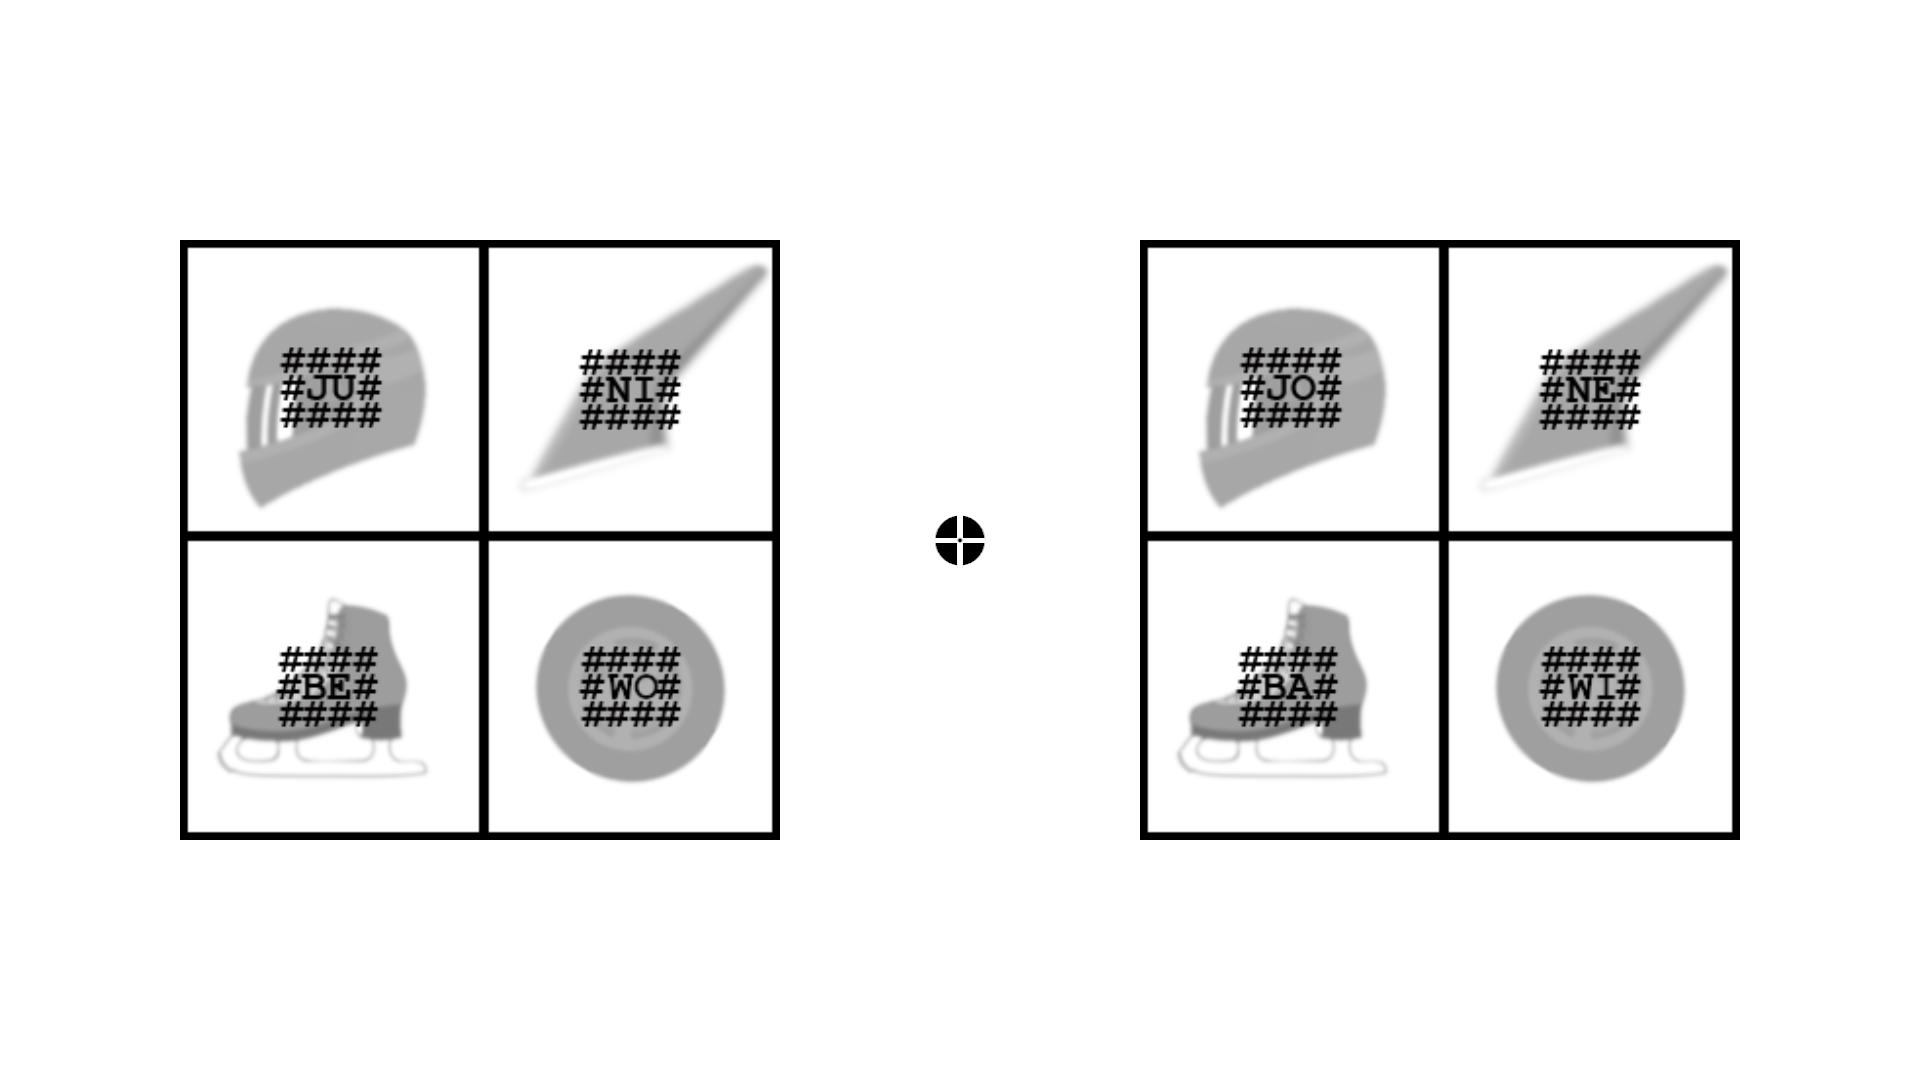
\includegraphics{C:/Users/rerr_/Google Drive/Graduate/Lab/Studies/MultiCue_Probabilistic/Stages/Shifted Weights/Eye Tracking/Analysis/Figures/Z_stimulus.png}
\caption{\label{fig:stimulus}Sample stimulus presented to participants.}
\end{figure}

\begin{figure}
\centering
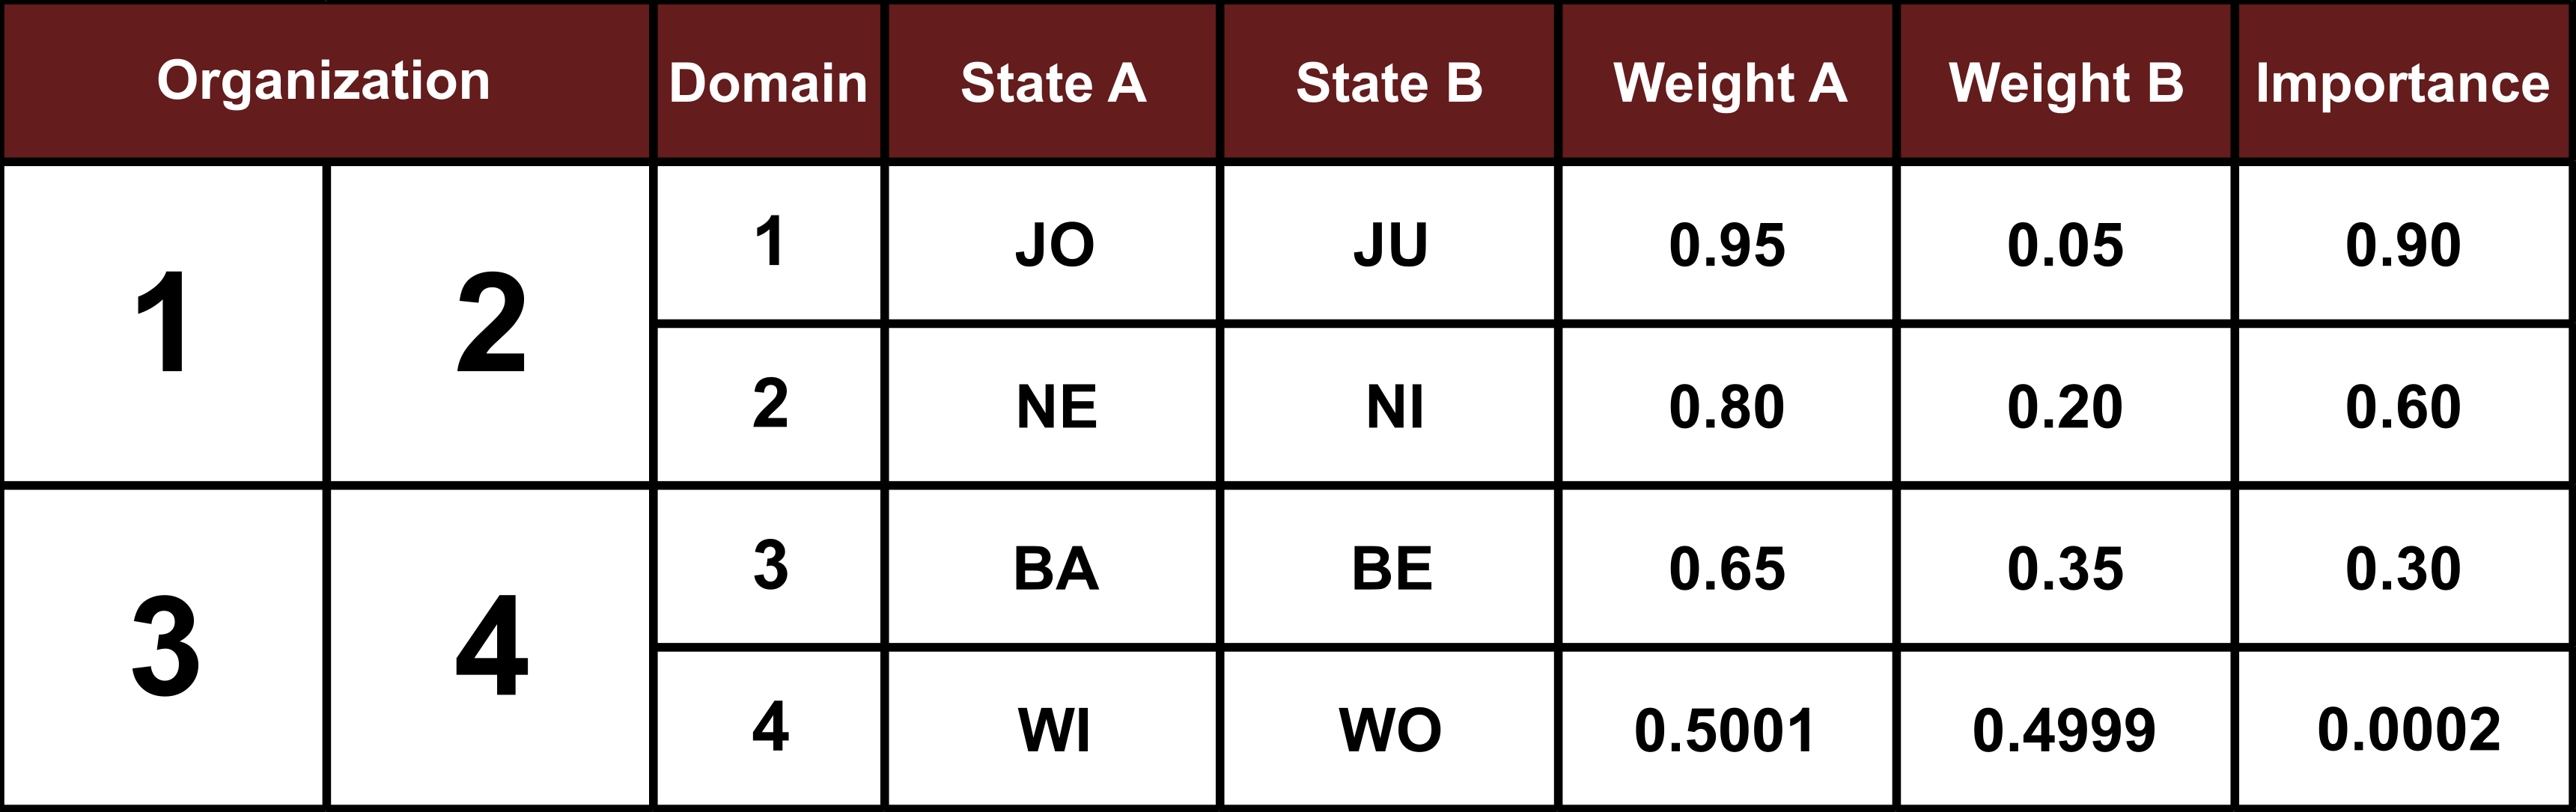
\includegraphics{C:/Users/rerr_/Google Drive/Graduate/Lab/Studies/MultiCue_Probabilistic/Stages/Shifted Weights/Eye Tracking/Analysis/Figures/Z_weights_normal.png}
\caption{\label{fig:weights}Example of the organization of cue weights across domains during training and T1. All the equipment (domains) and brands (states) kept their position constant across subjects, but the allocation of weights was assigned semirandomly across them.}
\end{figure}

\begin{figure}
\centering
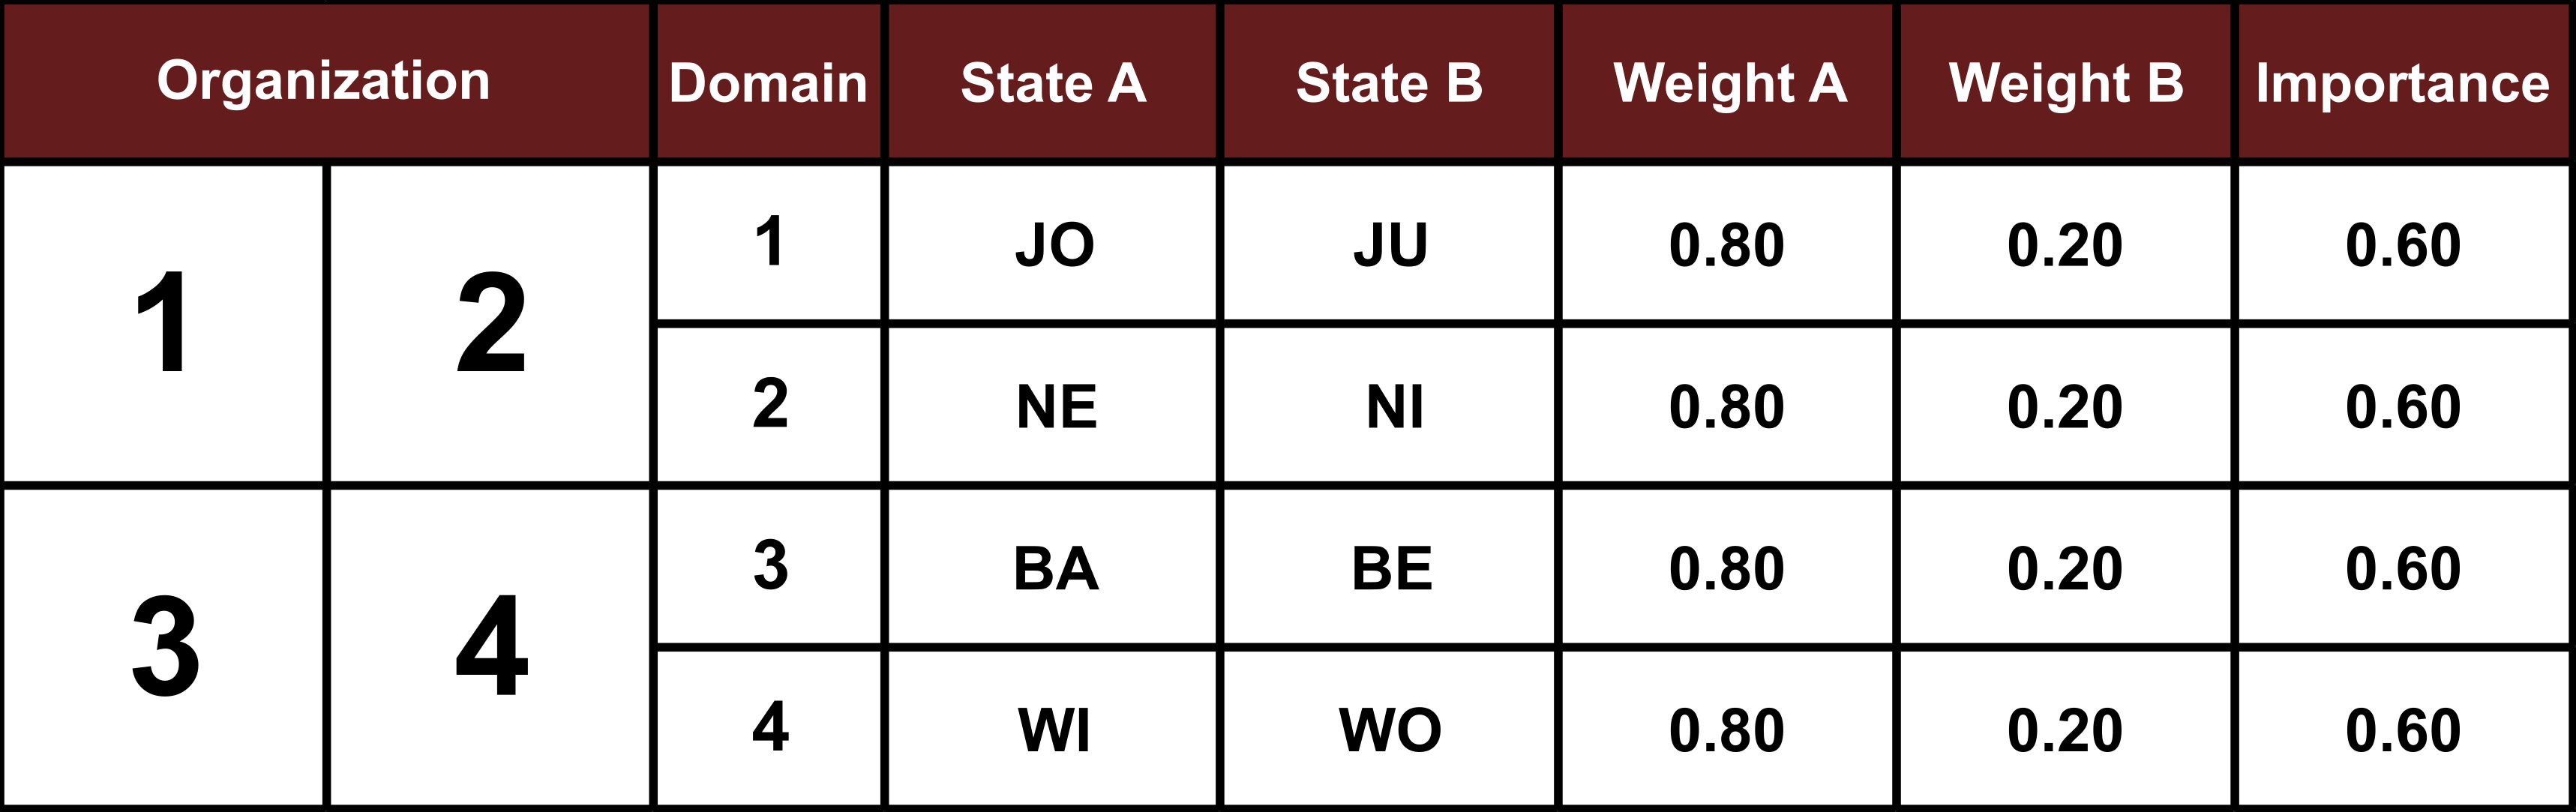
\includegraphics{C:/Users/rerr_/Google Drive/Graduate/Lab/Studies/MultiCue_Probabilistic/Stages/Shifted Weights/Eye Tracking/Analysis/Figures/Z_weights_equal.png}
\caption{\label{fig:weights-equal}Example of the organization of cue weights across domains during T2 in 0. All the different pairs had the same contingencies, preserving winning states.}
\end{figure}

\begin{figure}
\centering
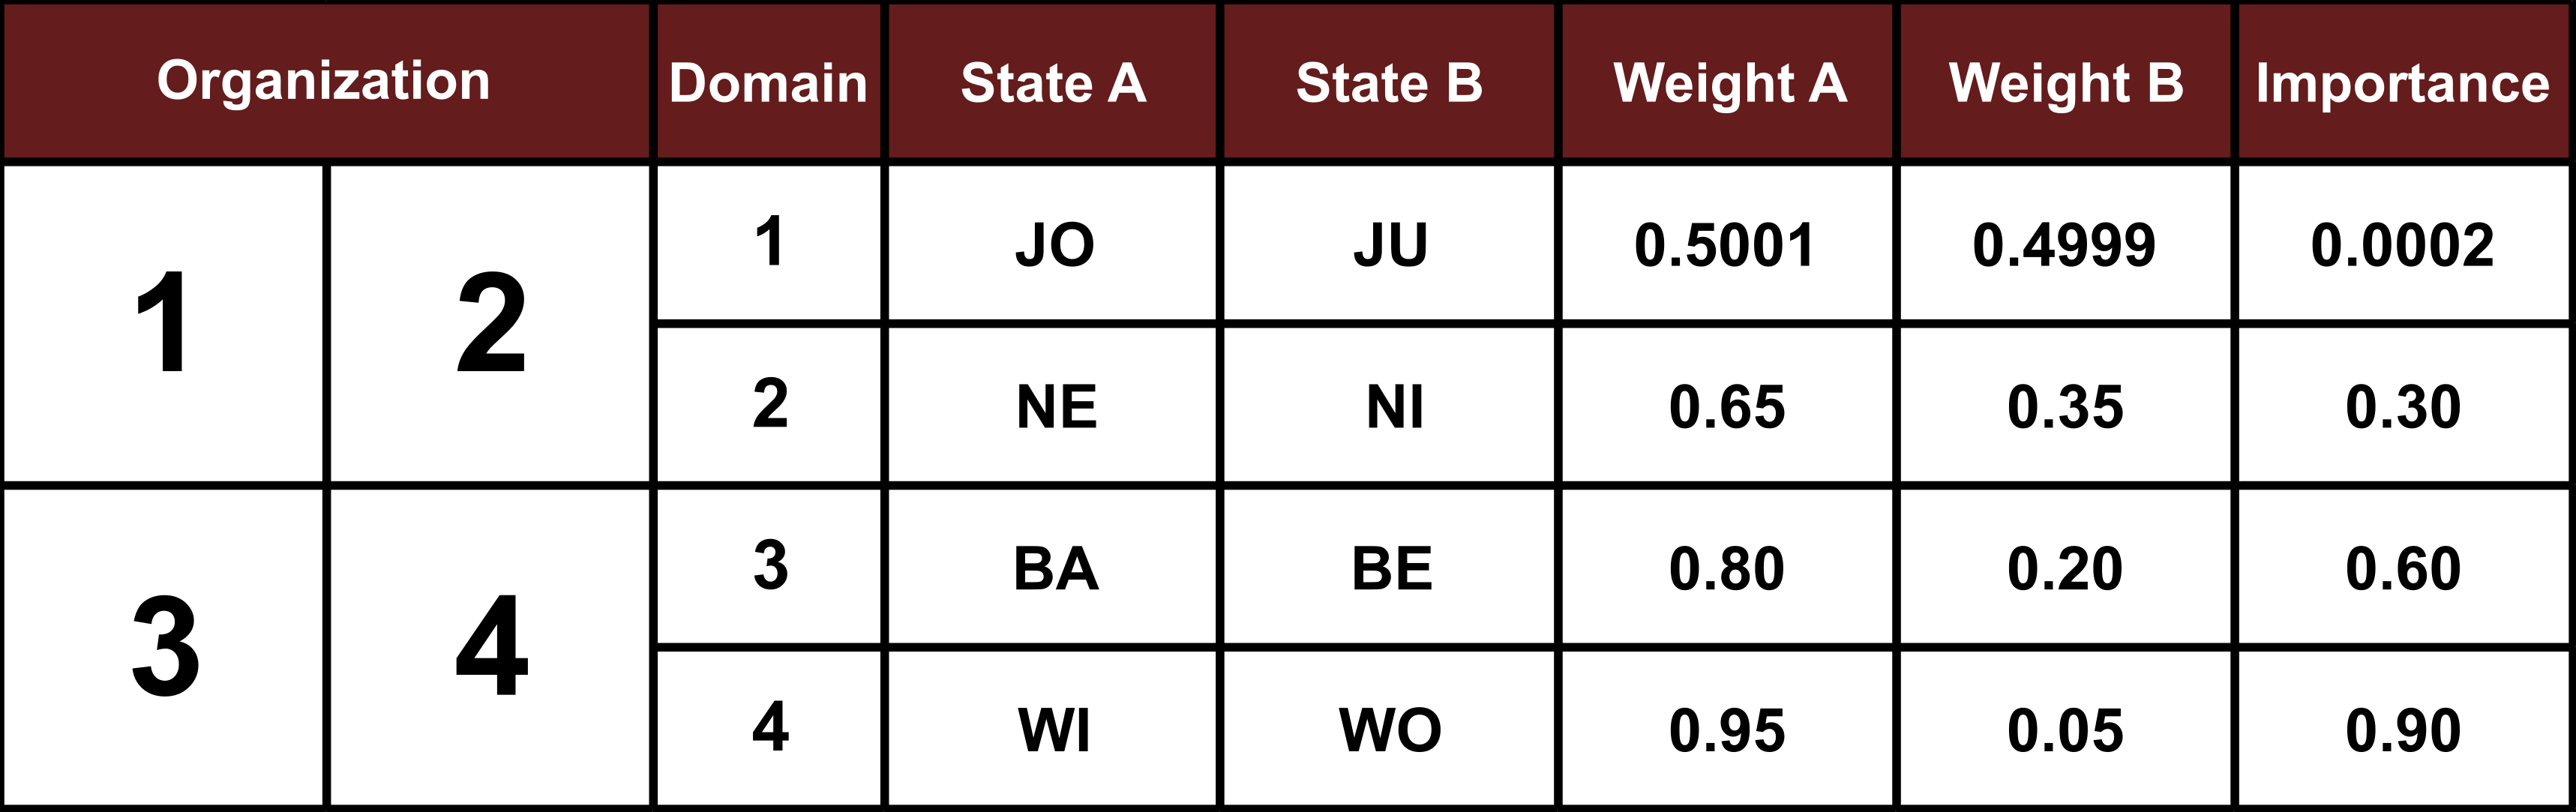
\includegraphics{C:/Users/rerr_/Google Drive/Graduate/Lab/Studies/MultiCue_Probabilistic/Stages/Shifted Weights/Eye Tracking/Analysis/Figures/Z_weights_inverted.png}
\caption{\label{fig:weights-inverted}Example of the organization of cue weights across domains during T2 in 1. The different domains show now inverted contingencies, preserving winning states.}
\end{figure}

\begin{figure}
\centering
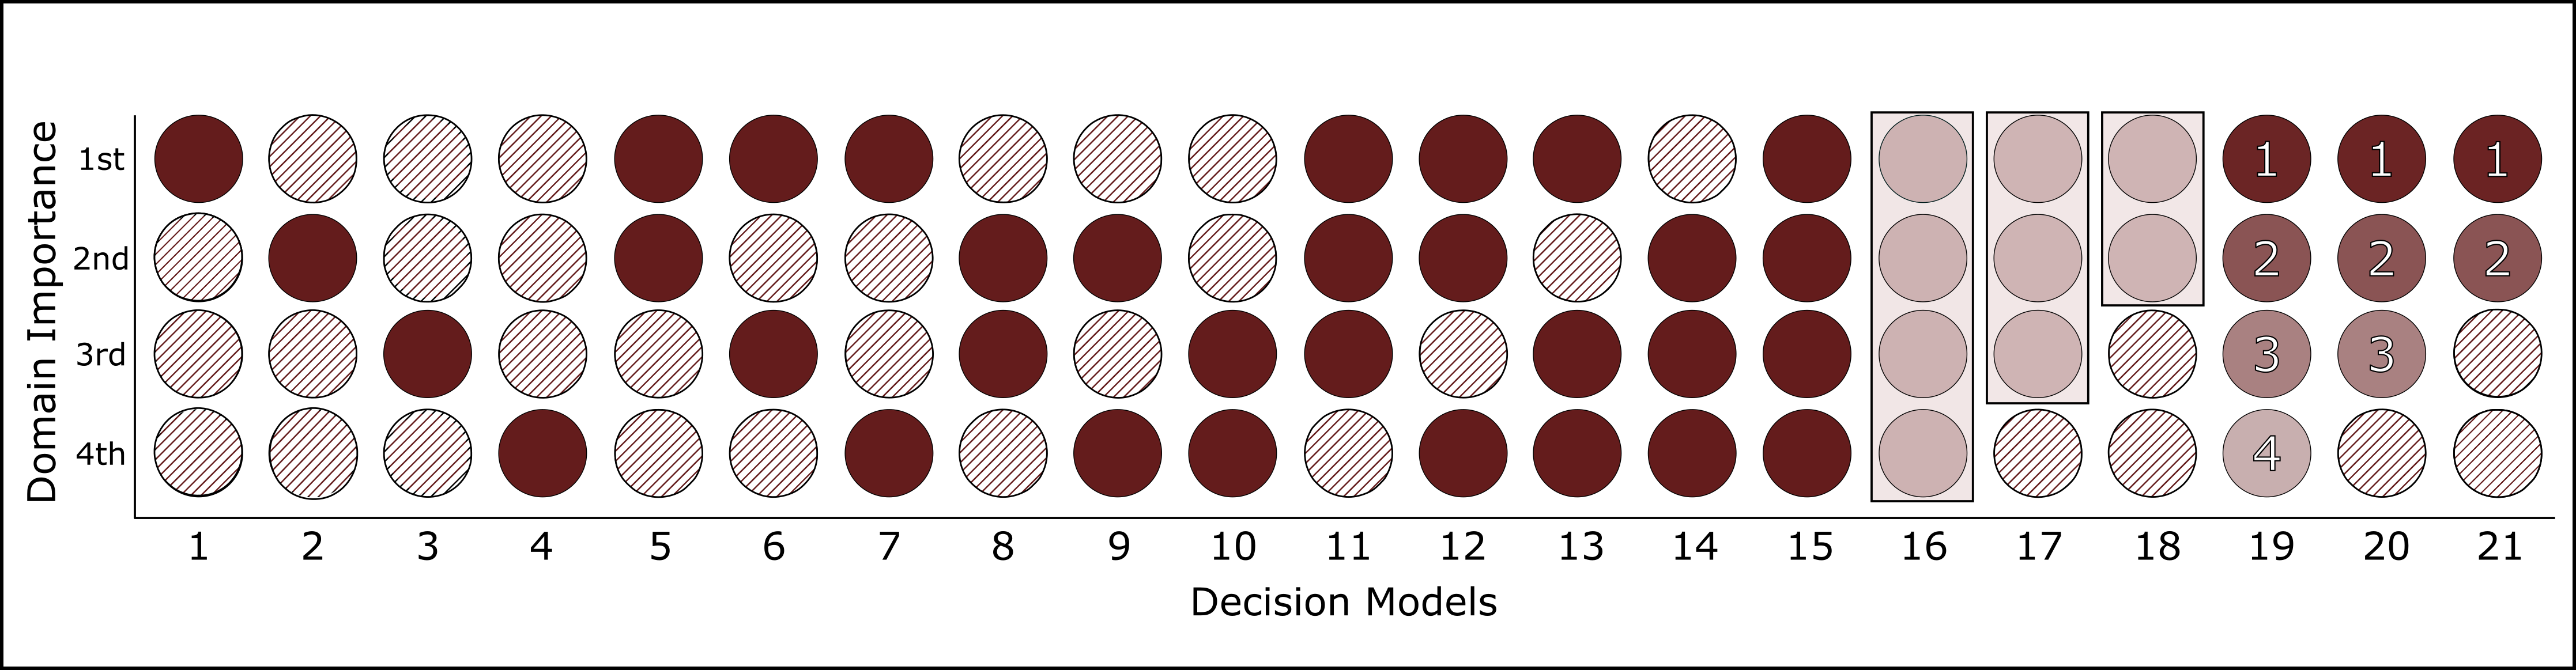
\includegraphics{C:/Users/rerr_/Google Drive/Graduate/Lab/Studies/MultiCue_Probabilistic/Stages/Shifted Weights/Eye Tracking/Analysis/Figures/Z_decision_models.png}
\caption{\label{fig:decision-models}Information usage in the different decision models. In models 1-15, black circles indicate the domain(s) used by each strategy. For models 16-18 we created a model that integrated the domains in a single piece of information (i.e.~a sum of positive traits). Models 19-21 consider a Serial Search for information, starting in the most informative domain, continuing in descending order of importance, and stoping as soon as any of these domains discriminates between cues.}
\end{figure}

\begin{figure}
\centering
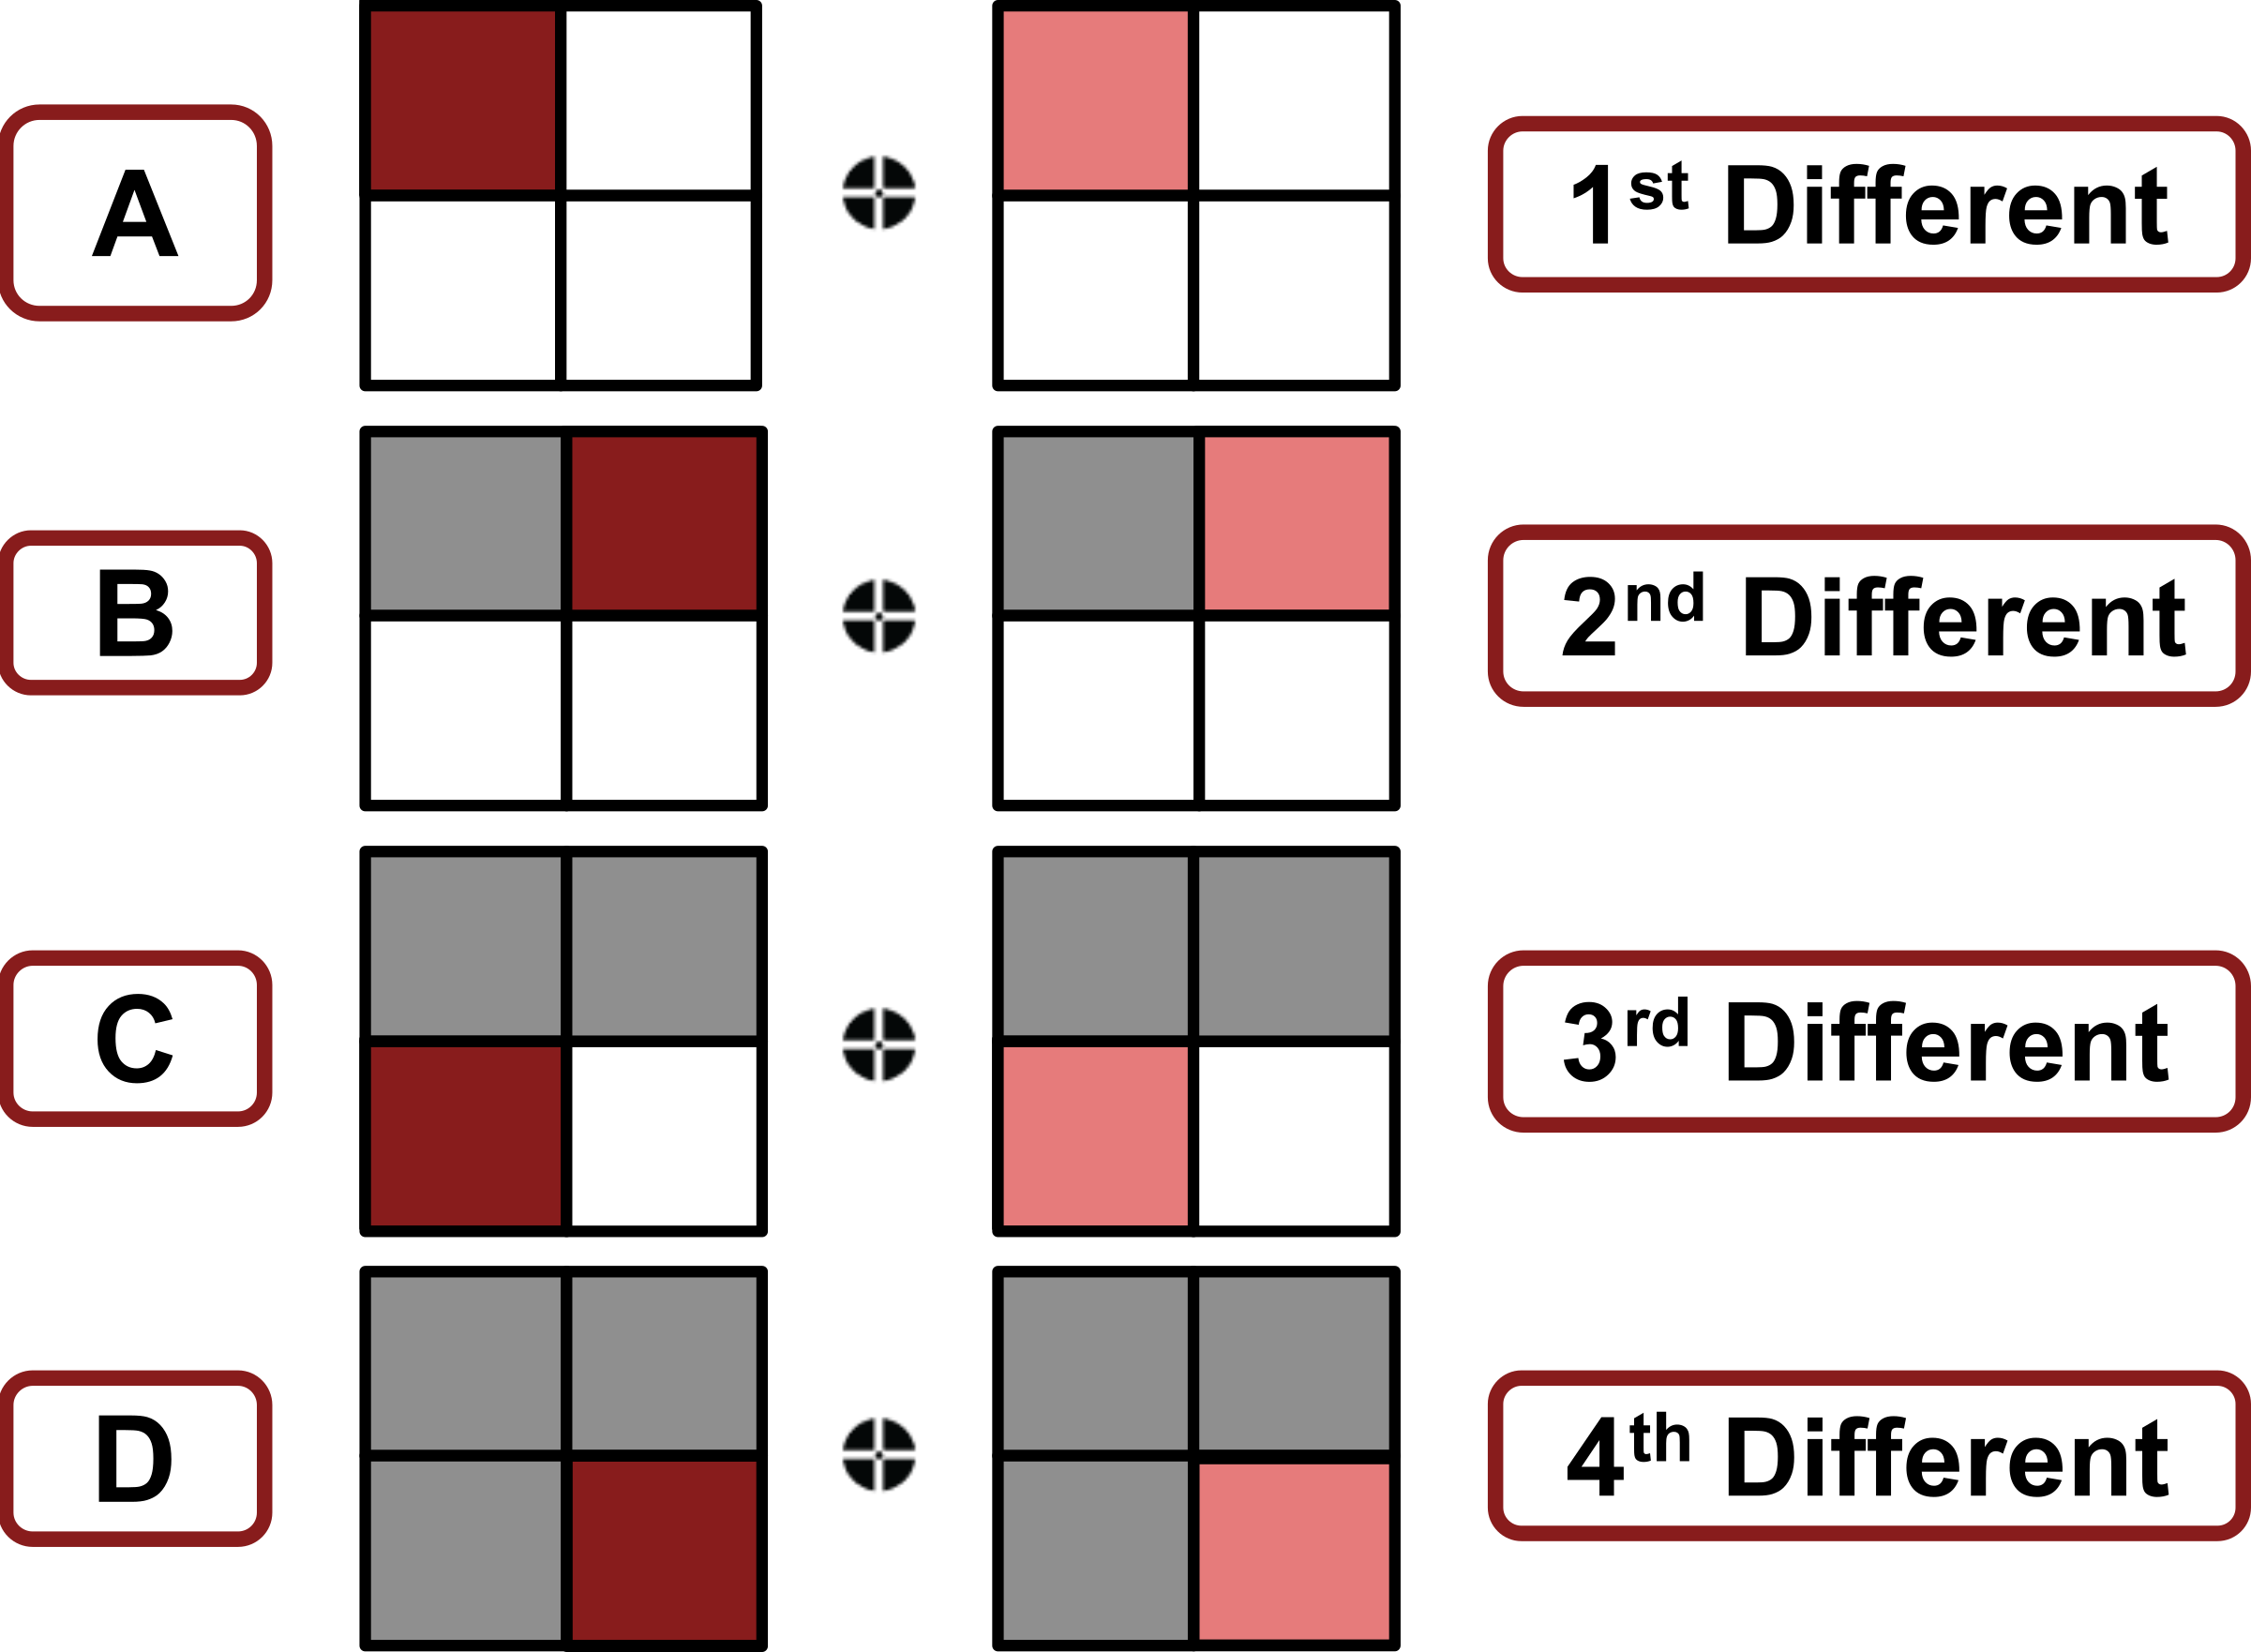
\includegraphics{C:/Users/rerr_/Google Drive/Graduate/Lab/Studies/MultiCue_Probabilistic/Stages/Shifted Weights/Eye Tracking/Analysis/Figures/Z_scenarios.png}
\caption{\label{fig:scenarios}Decision scenarios according to the best discriminating domain between cues.}
\end{figure}

\begin{figure}
\centering
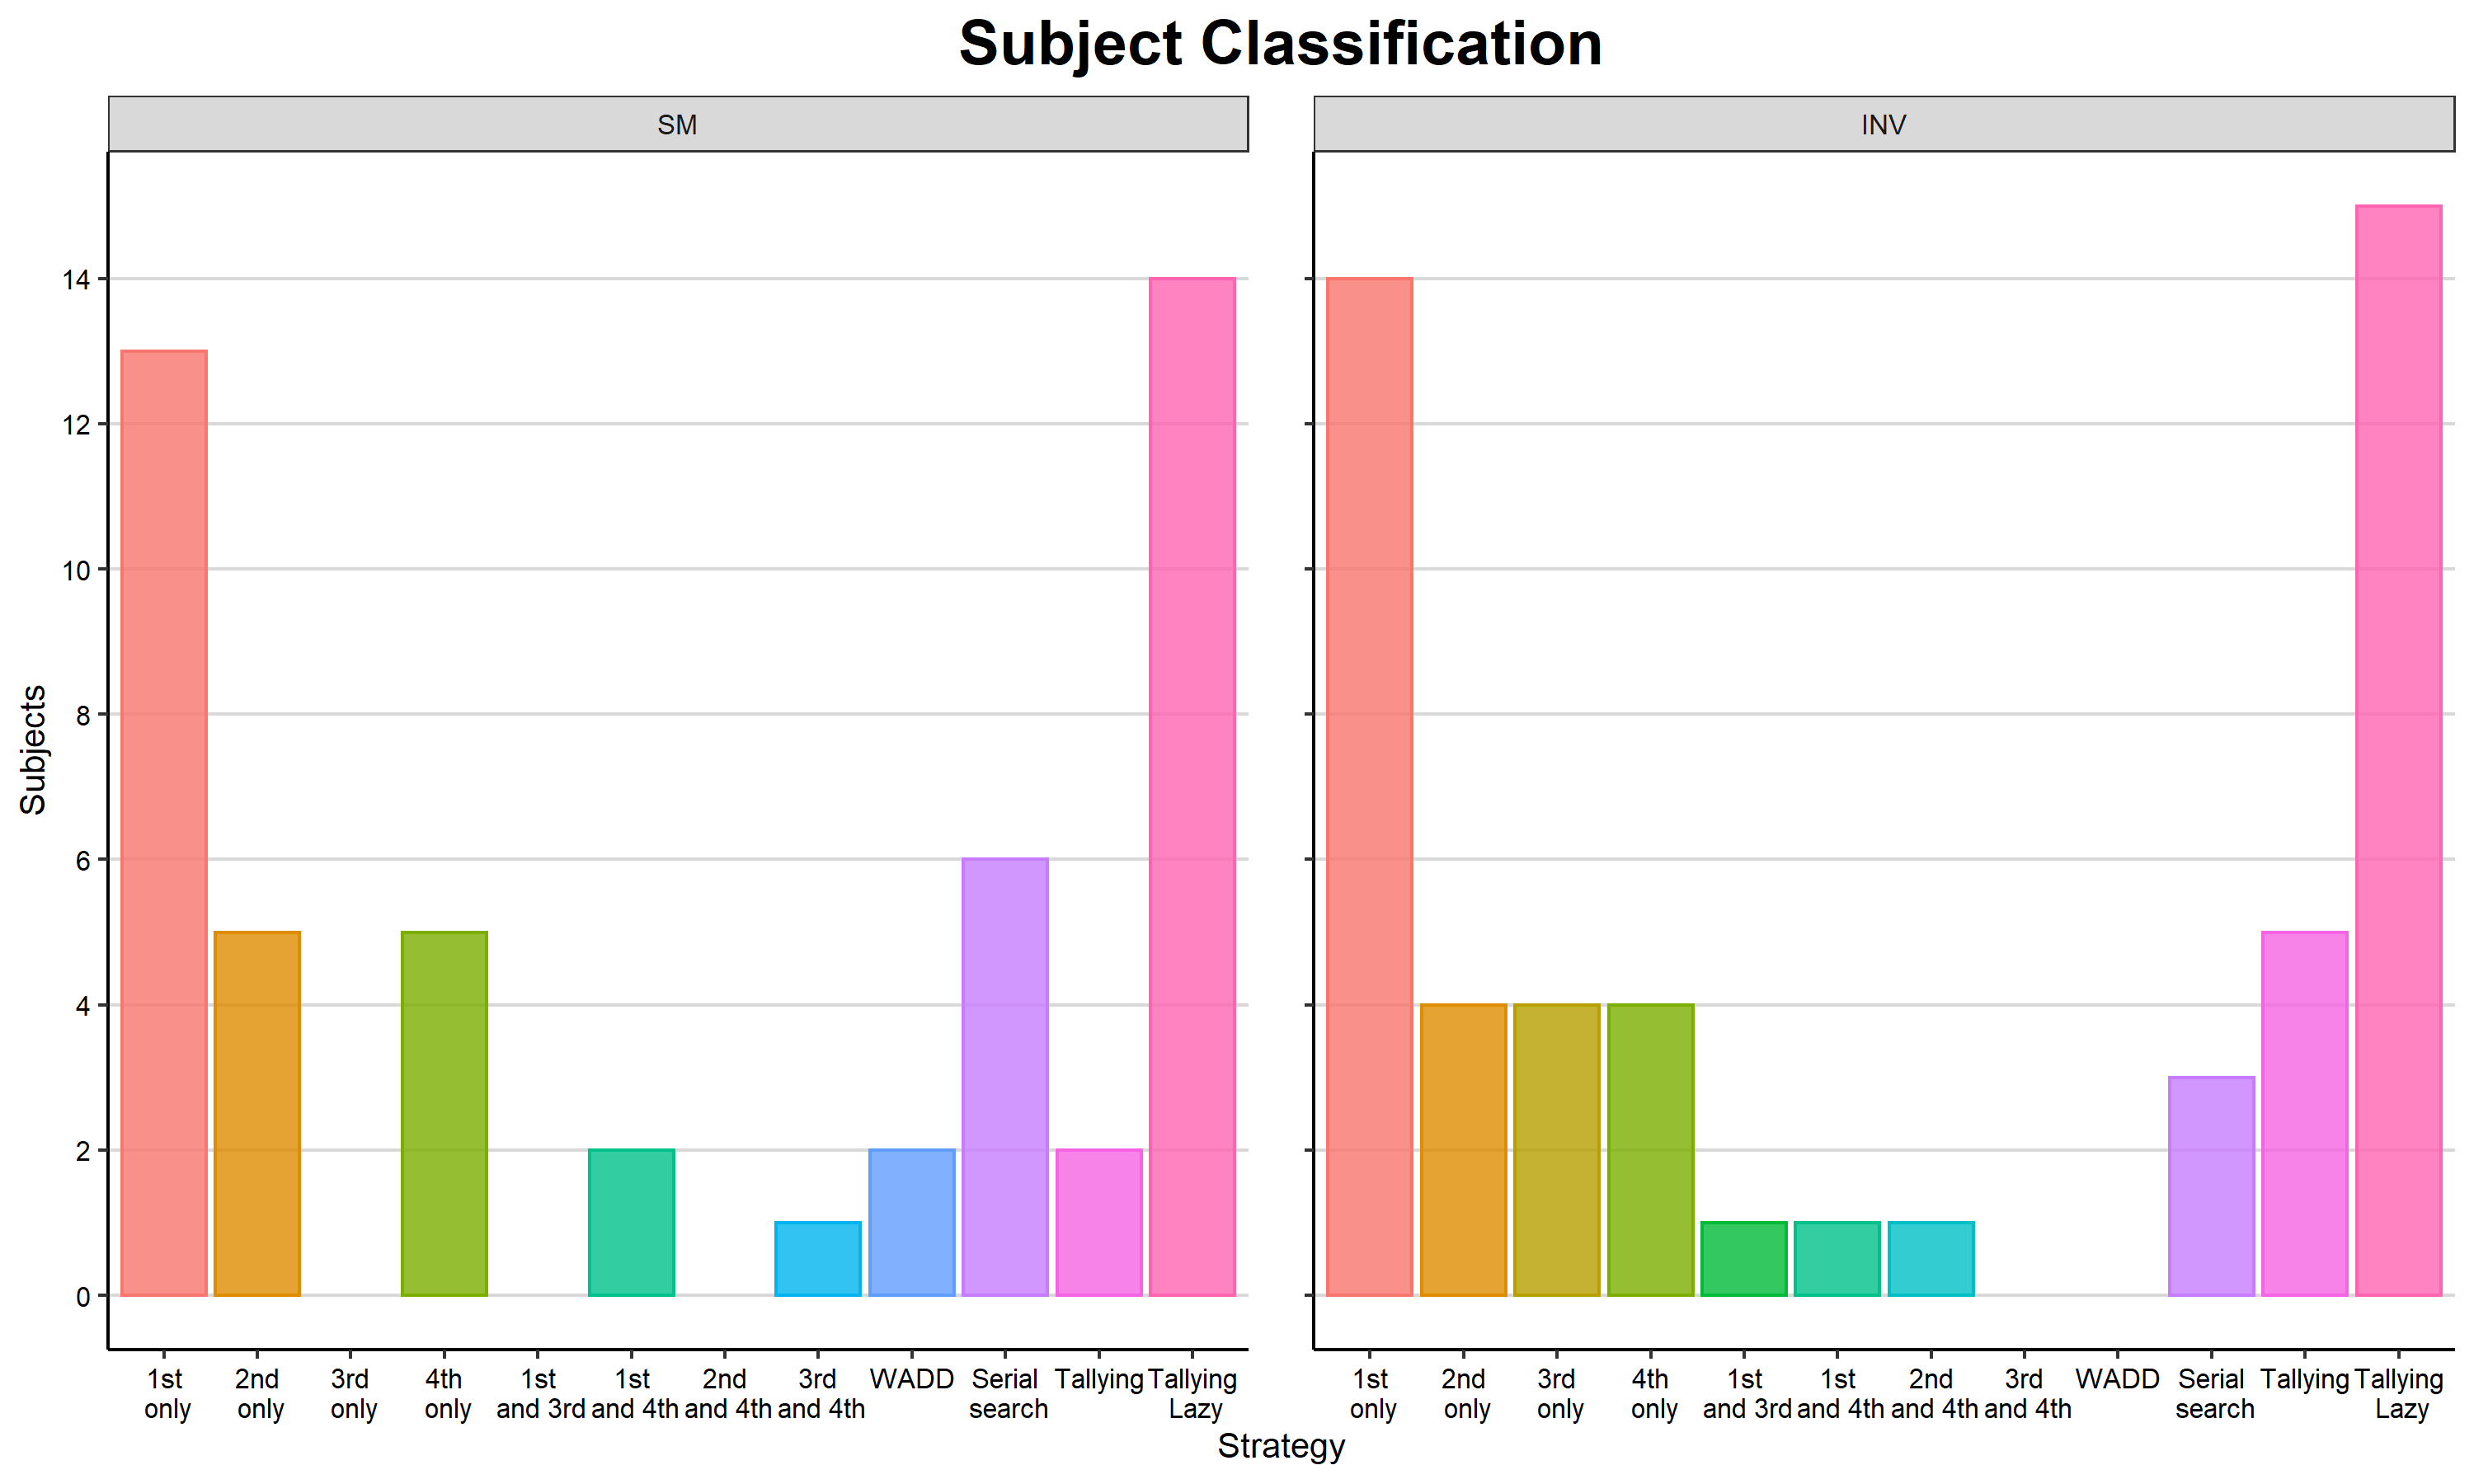
\includegraphics{C:/Users/rerr_/Google Drive/Graduate/Lab/Studies/MultiCue_Probabilistic/Stages/Shifted Weights/Eye Tracking/Analysis/Figures/A1_model_histogram.png}
\caption{\label{fig:classification}Strategy group classification based on the variational Bayesian inference.}
\end{figure}

\begin{figure}
\centering
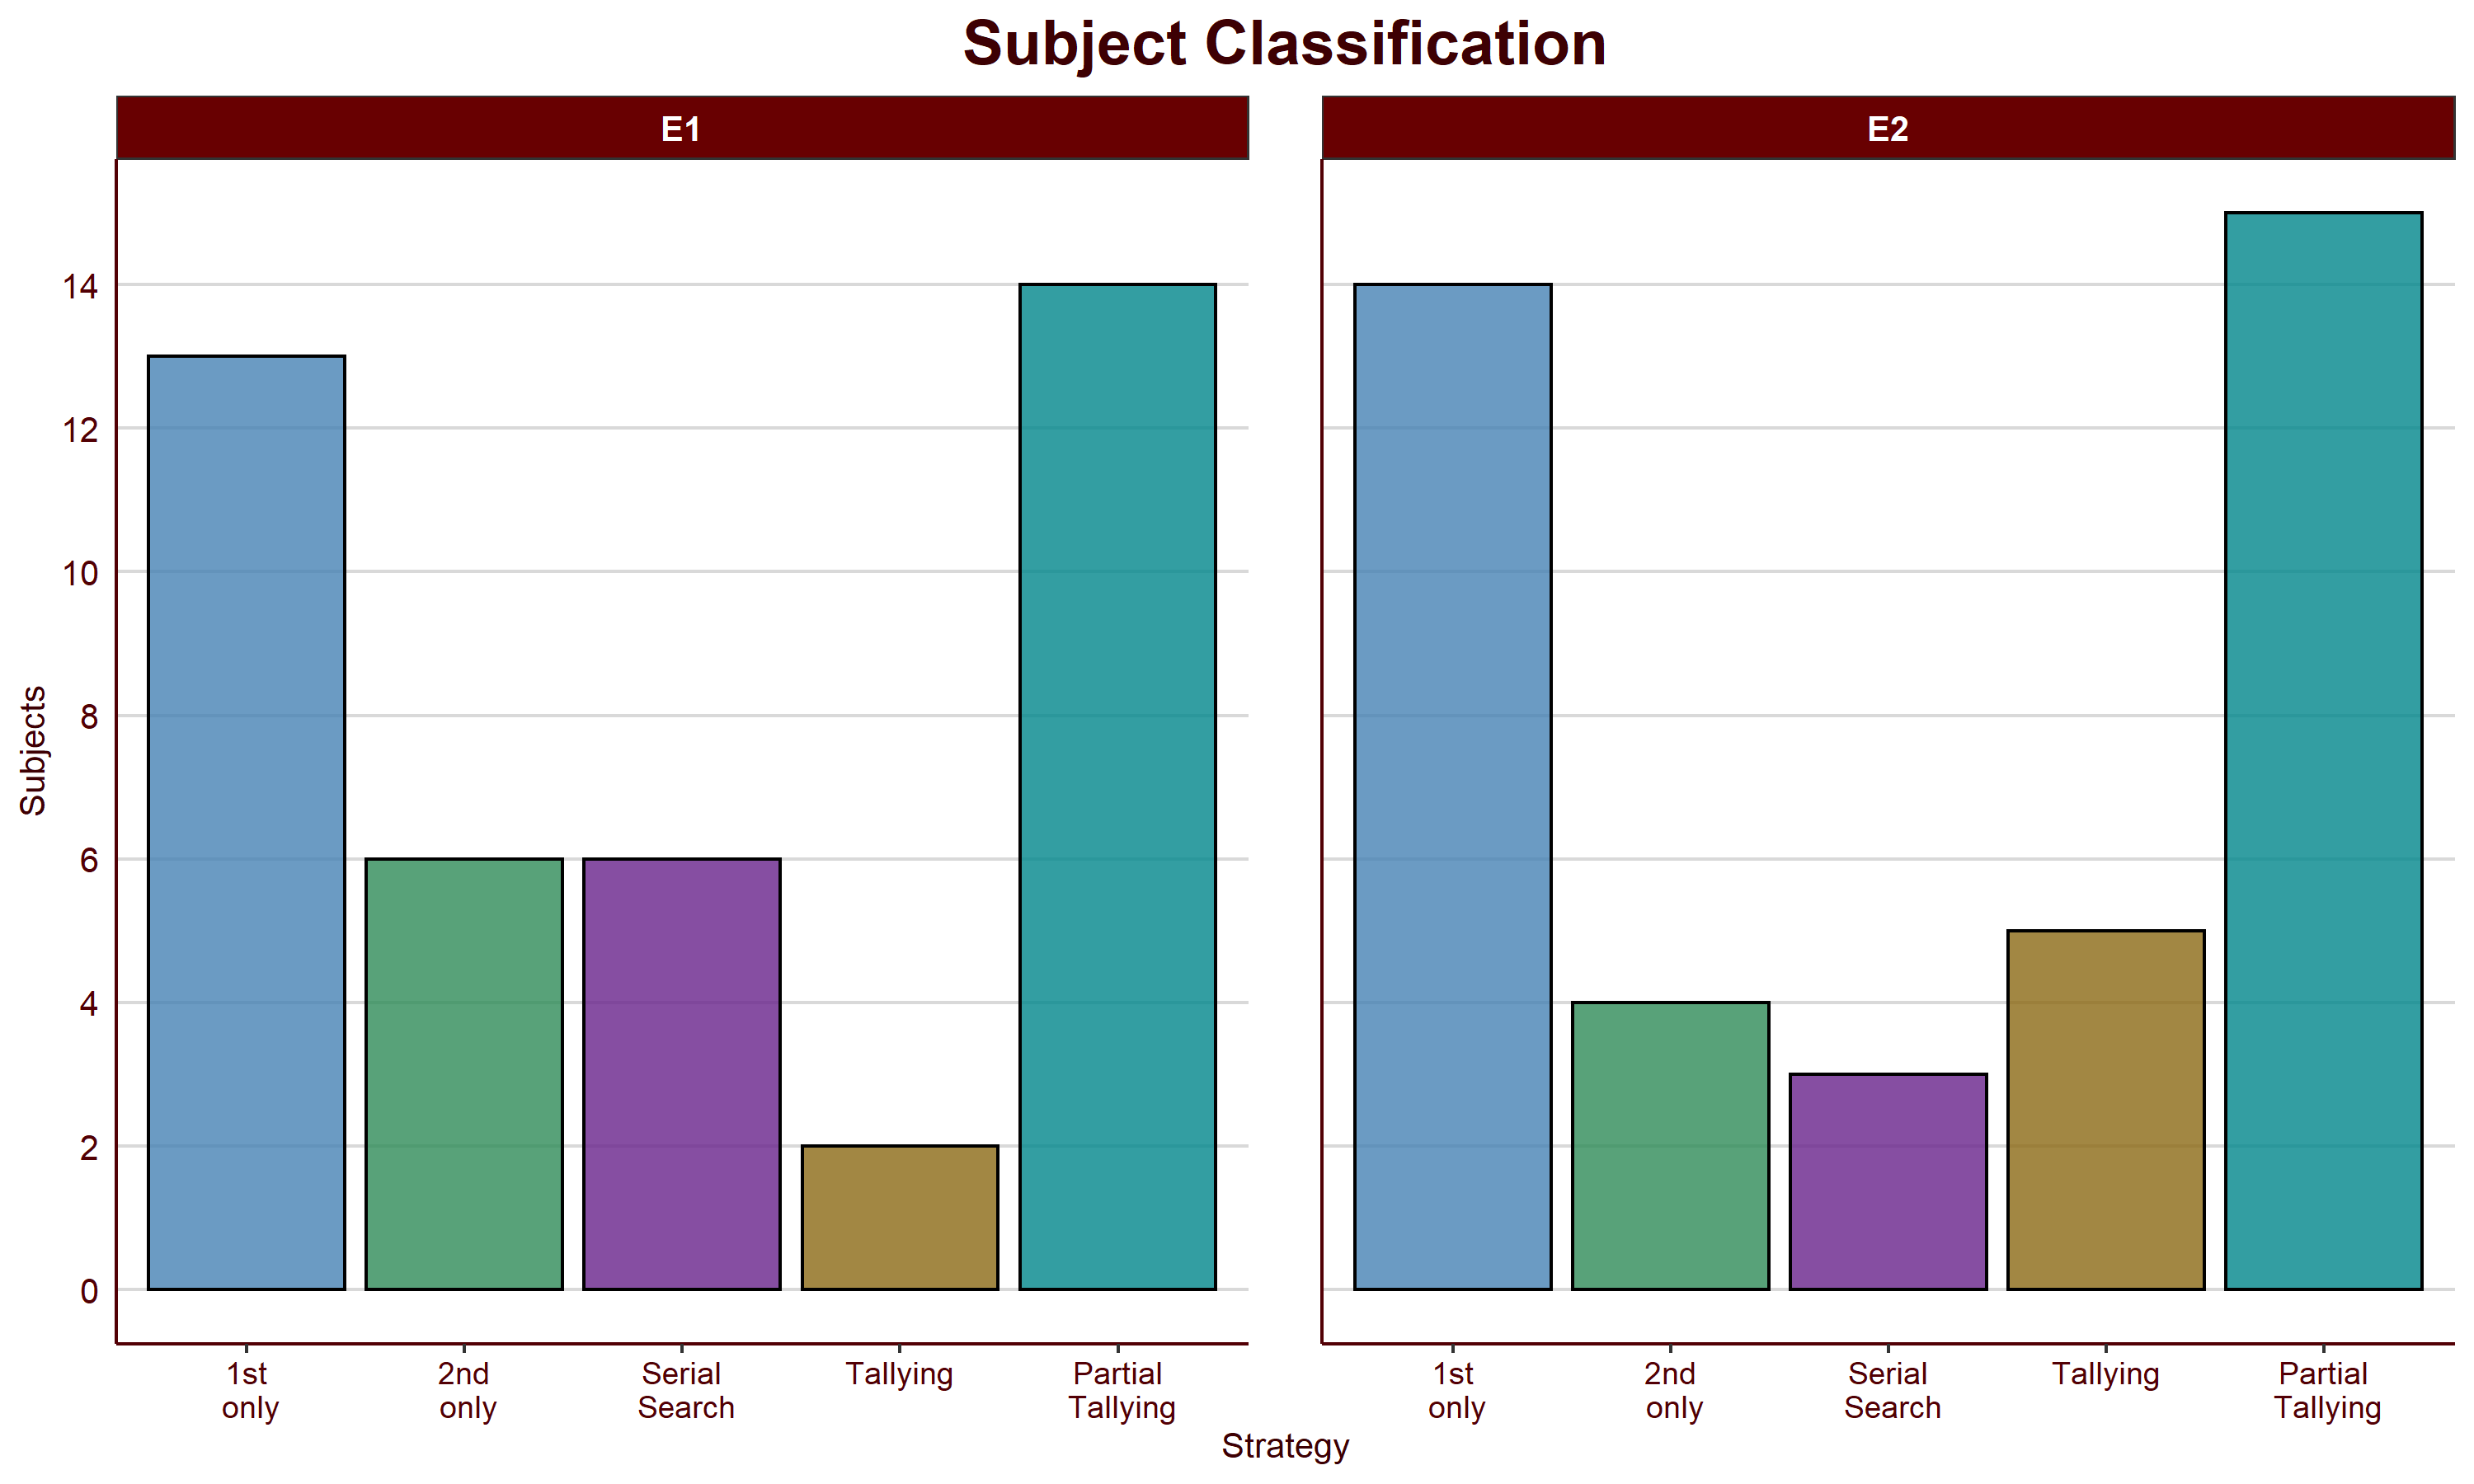
\includegraphics{C:/Users/rerr_/Google Drive/Graduate/Lab/Studies/MultiCue_Probabilistic/Stages/Shifted Weights/Eye Tracking/Analysis/Figures/A2_model_histogram.png}
\caption{\label{fig:classification-reduced}Decision groups studied in detail for this work.}
\end{figure}

\begin{figure}
\centering
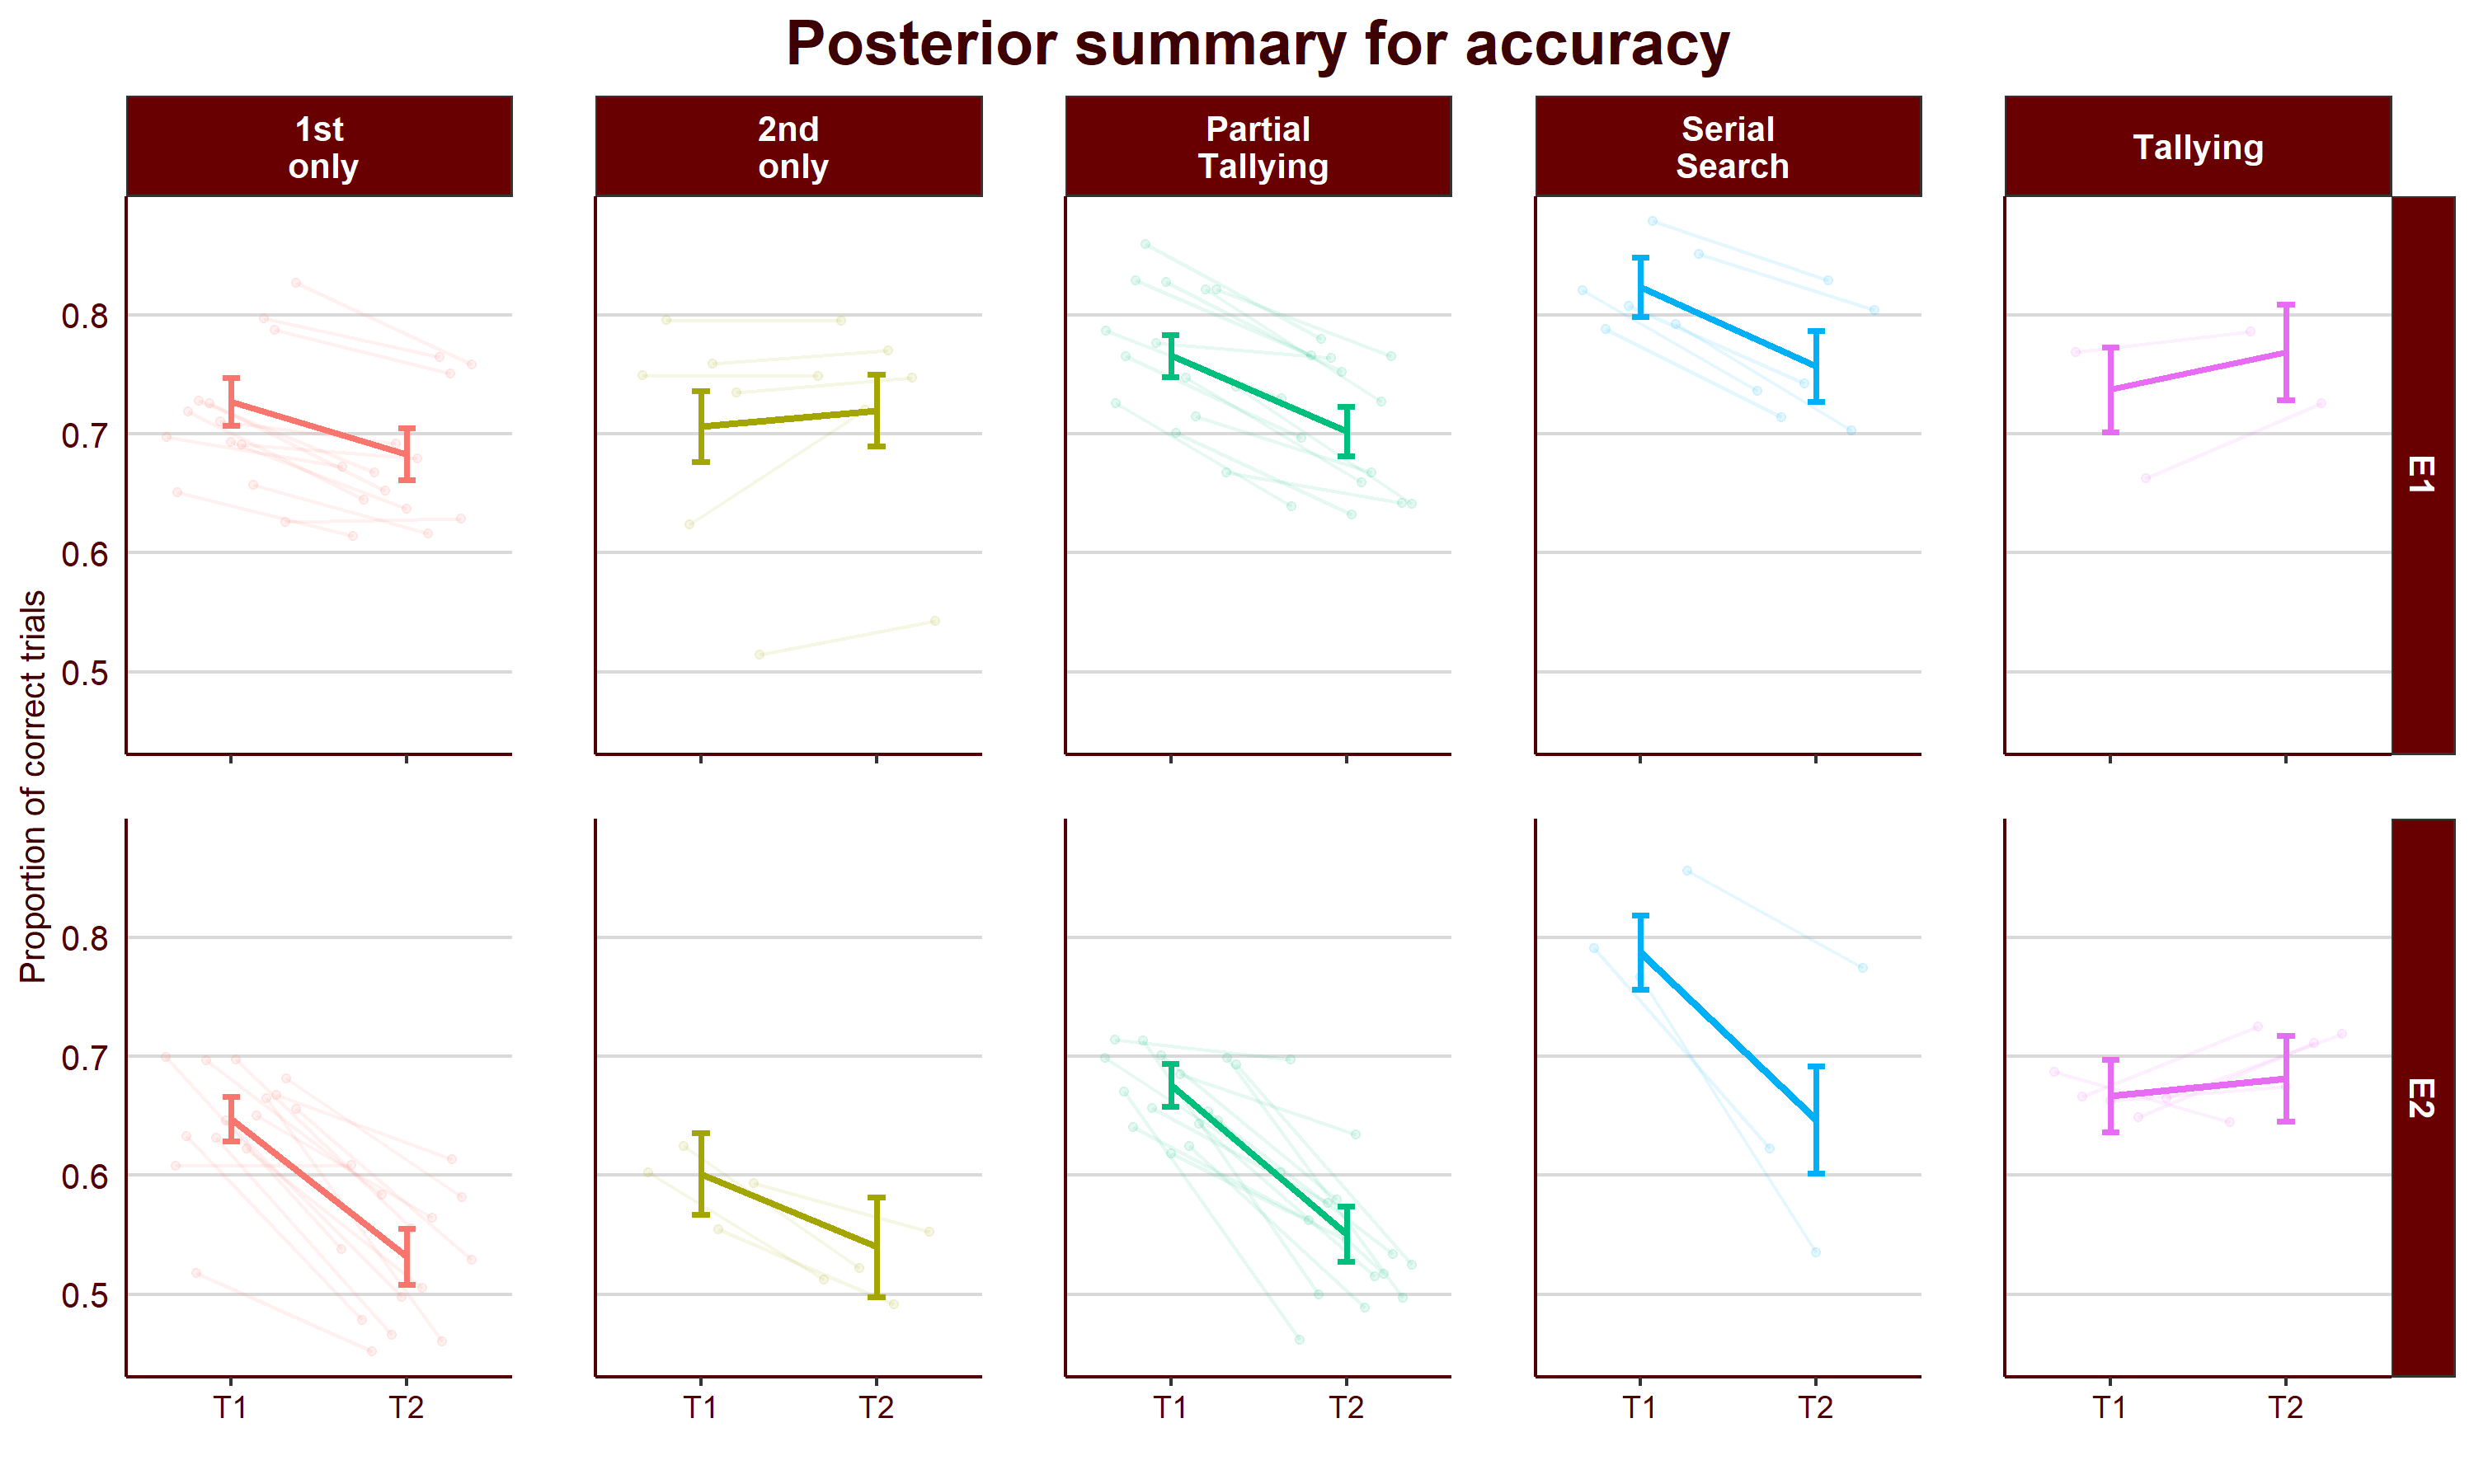
\includegraphics{C:/Users/rerr_/Google Drive/Graduate/Lab/Studies/MultiCue_Probabilistic/Stages/Shifted Weights/Eye Tracking/Analysis/Figures/B1_performance.png}
\caption{\label{fig:performance}Performance (as percent of accurate trials) across testing phases. Individual dots correspond to the median from the posterior draws from each participant. Error bars represent standard deviations.}
\end{figure}

\begin{center}
\begin{ThreePartTable}

\begin{longtable}{llllll}\noalign{\getlongtablewidth\global\LTcapwidth=\longtablewidth}
\caption{\label{tab:table-performance-change}Accuracy between phases across groups}\\
\toprule
experiment & \multicolumn{1}{c}{strategy} & \multicolumn{1}{c}{ROPE\_Percentage} & \multicolumn{1}{c}{rawdirection} & \multicolumn{1}{c}{p\_HDI} & \multicolumn{1}{c}{p\_direction}\\
\midrule
\endfirsthead
\caption*{\normalfont{Table \ref{tab:table-performance-change} continued}}\\
\toprule
experiment & \multicolumn{1}{c}{strategy} & \multicolumn{1}{c}{ROPE\_Percentage} & \multicolumn{1}{c}{rawdirection} & \multicolumn{1}{c}{p\_HDI} & \multicolumn{1}{c}{p\_direction}\\
\midrule
\endhead
0 & 1st only & 0.35 & 0.99 & 35.30\% & = 0.987\\
0 & 2nd only & 0.83 & 0.68 & 82.80\% & = 0.681\\
0 & Partial Tallying & 0.02 & 1.00 & 2.10\% & > 0.999\\
0 & Serial Search & 0.02 & 1.00 & 1.60\% & = 0.997\\
0 & Tallying & 0.50 & 0.79 & 49.60\% & = 0.789\\
1 & 1st only & 0.00 & 1.00 & 0.00\% & > 0.999\\
1 & 2nd only & 0.33 & 0.94 & 33.00\% & = 0.936\\
1 & Partial Tallying & 0.00 & 1.00 & 0.00\% & > 0.999\\
1 & Serial Search & 0.00 & 1.00 & 0.00\% & > 0.999\\
1 & Tallying & 0.74 & 0.65 & 73.80\% & = 0.652\\
\bottomrule
\end{longtable}

\end{ThreePartTable}
\end{center}

\begin{center}
\begin{ThreePartTable}

\begin{longtable}{llllll}\noalign{\getlongtablewidth\global\LTcapwidth=\longtablewidth}
\caption{\label{tab:table-performance-group-diff}Paired comparisons between groups on the difference in performance across phases}\\
\toprule
experiment & \multicolumn{1}{c}{comparison} & \multicolumn{1}{c}{ROPE\_Percentage} & \multicolumn{1}{c}{rawdirection} & \multicolumn{1}{c}{p\_HDI} & \multicolumn{1}{c}{p\_direction}\\
\midrule
\endfirsthead
\caption*{\normalfont{Table \ref{tab:table-performance-group-diff} continued}}\\
\toprule
experiment & \multicolumn{1}{c}{comparison} & \multicolumn{1}{c}{ROPE\_Percentage} & \multicolumn{1}{c}{rawdirection} & \multicolumn{1}{c}{p\_HDI} & \multicolumn{1}{c}{p\_direction}\\
\midrule
\endhead
0 & first\_lazy & 0.74 & 0.82 & 74.2\% & = 0.824\\
0 & first\_second & 0.24 & 0.96 & 24.2\% & = 0.958\\
0 & first\_serial & 0.47 & 0.87 & 46.9\% & = 0.874\\
0 & first\_tally & 0.17 & 0.95 & 16.7\% & = 0.954\\
0 & second\_lazy & 0.06 & 0.99 & 5.8\% & = 0.989\\
0 & second\_serial & 0.04 & 0.98 & 3.6\% & = 0.985\\
0 & second\_tally & 0.60 & 0.69 & 59.7\% & = 0.688\\
0 & serial\_lazy & 0.75 & 0.69 & 75.4\% & = 0.689\\
0 & serial\_tally & 0.02 & 0.98 & 2.4\% & = 0.984\\
0 & tally\_lazy & 0.04 & 0.98 & 3.6\% & = 0.983\\
1 & first\_lazy & 0.88 & 0.66 & 87.9\% & = 0.664\\
1 & first\_second & 0.36 & 0.89 & 36.5\% & = 0.89\\
1 & first\_serial & 0.40 & 0.86 & 39.9\% & = 0.862\\
1 & first\_tally & 0.00 & 1.00 & 0.0\% & = 0.997\\
1 & second\_lazy & 0.26 & 0.92 & 25.6\% & = 0.922\\
1 & second\_serial & 0.08 & 0.96 & 8.5\% & = 0.96\\
1 & second\_tally & 0.28 & 0.91 & 27.5\% & = 0.913\\
1 & serial\_lazy & 0.54 & 0.80 & 53.5\% & = 0.796\\
1 & serial\_tally & 0.00 & 1.00 & 0.0\% & = 0.998\\
1 & tally\_lazy & 0.00 & 1.00 & 0.0\% & = 0.998\\
\bottomrule
\end{longtable}

\end{ThreePartTable}
\end{center}

\begin{center}
\begin{ThreePartTable}

\begin{longtable}{lllll}\noalign{\getlongtablewidth\global\LTcapwidth=\longtablewidth}
\caption{\label{tab:table-performance-T1}Paired comparisons between groups on the performance in T1}\\
\toprule
comparison & \multicolumn{1}{c}{ROPE\_Percentage} & \multicolumn{1}{c}{rawdirection} & \multicolumn{1}{c}{p\_HDI} & \multicolumn{1}{c}{p\_direction}\\
\midrule
\endfirsthead
\caption*{\normalfont{Table \ref{tab:table-performance-T1} continued}}\\
\toprule
comparison & \multicolumn{1}{c}{ROPE\_Percentage} & \multicolumn{1}{c}{rawdirection} & \multicolumn{1}{c}{p\_HDI} & \multicolumn{1}{c}{p\_direction}\\
\midrule
\endhead
first\_lazy & 0.82 & 0.74 & 81.60\% & = 0.739\\
first\_second & 0.65 & 0.72 & 65.20\% & = 0.715\\
first\_serial & 0.07 & 0.98 & 6.60\% & = 0.981\\
first\_tally & 0.00 & 0.98 & 0.30\% & = 0.983\\
second\_lazy & 0.74 & 0.56 & 73.50\% & = 0.556\\
second\_serial & 0.30 & 0.88 & 29.90\% & = 0.883\\
second\_tally & 0.15 & 0.93 & 15.40\% & = 0.927\\
serial\_lazy & 0.19 & 0.95 & 18.90\% & = 0.952\\
serial\_tally & 0.52 & 0.67 & 52.10\% & = 0.668\\
tally\_lazy & 0.07 & 0.96 & 7.00\% & = 0.962\\
\bottomrule
\end{longtable}

\end{ThreePartTable}
\end{center}

\begin{figure}
\centering
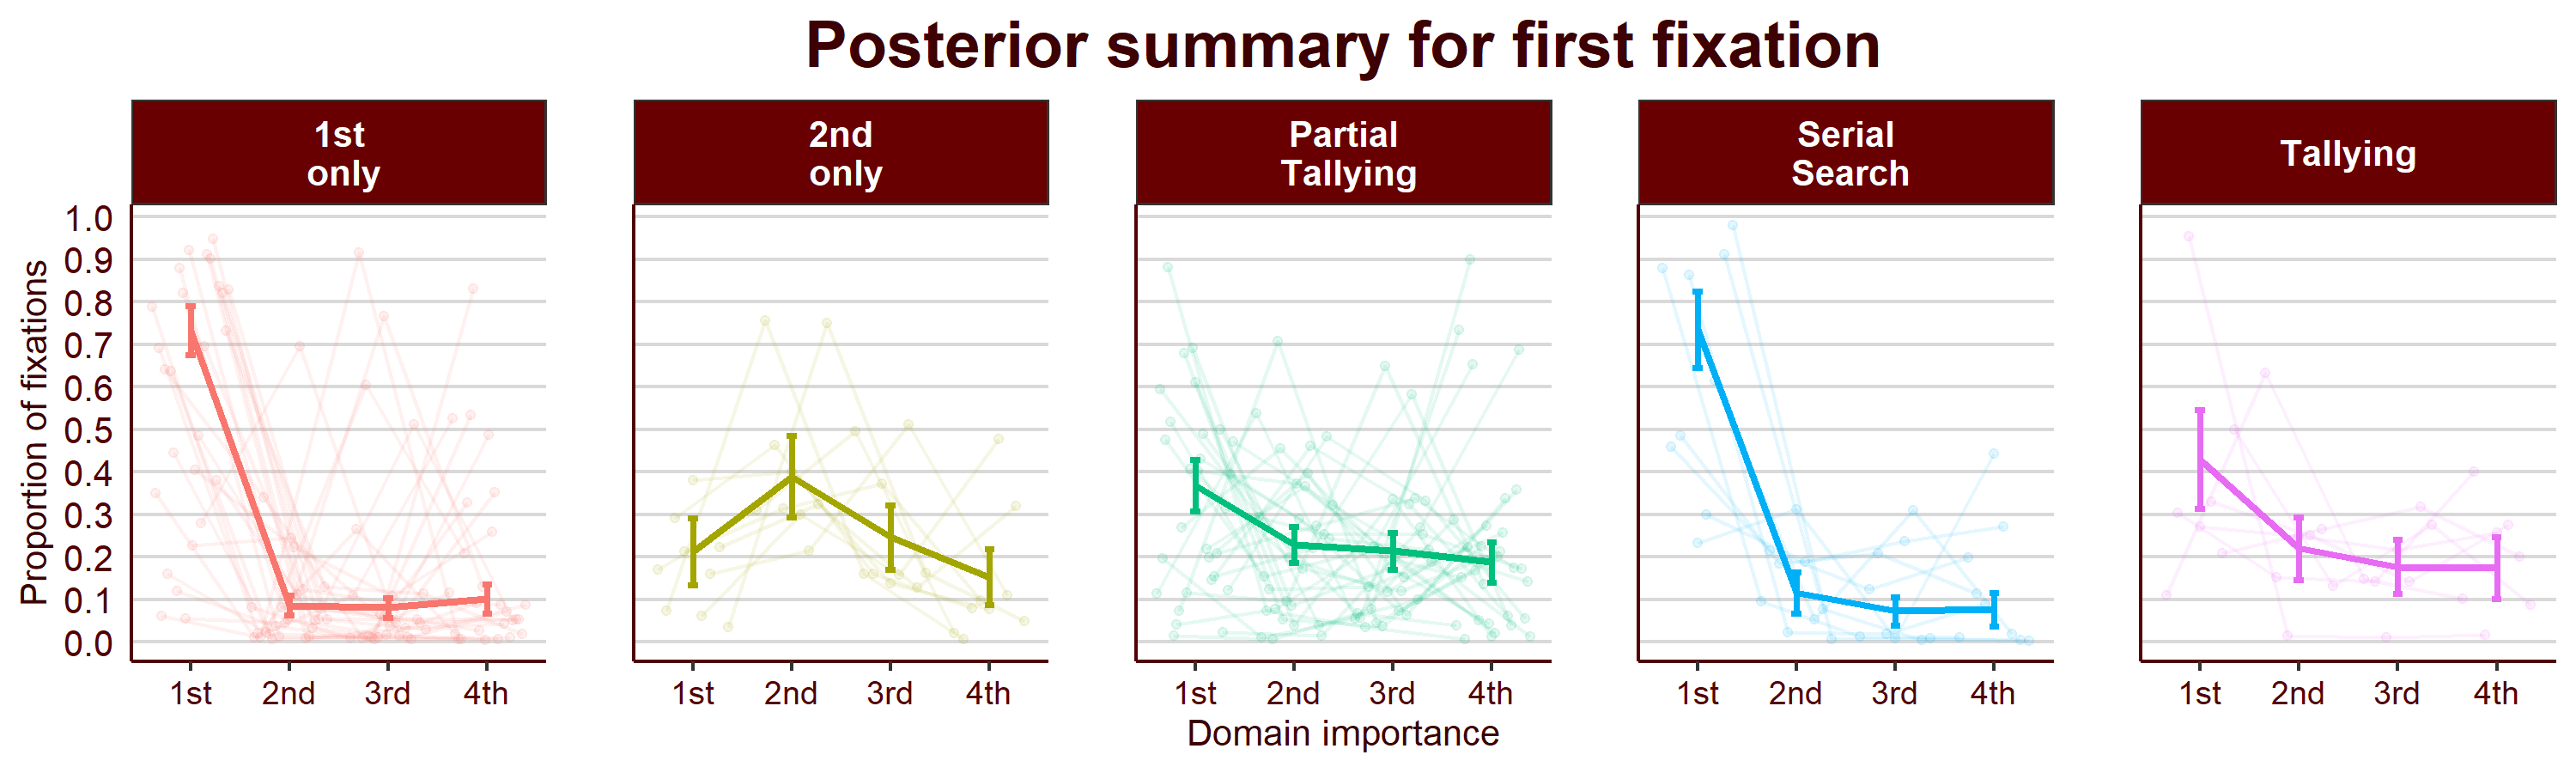
\includegraphics{C:/Users/rerr_/Google Drive/Graduate/Lab/Studies/MultiCue_Probabilistic/Stages/Shifted Weights/Eye Tracking/Analysis/Figures/C1_first.png}
\caption{\label{fig:first}Allocation of first fixations across domains in T1. Individual dots correspond to the median from the posterior draws from each participant. Error bars represent standard deviations.}
\end{figure}

\begin{figure}
\centering
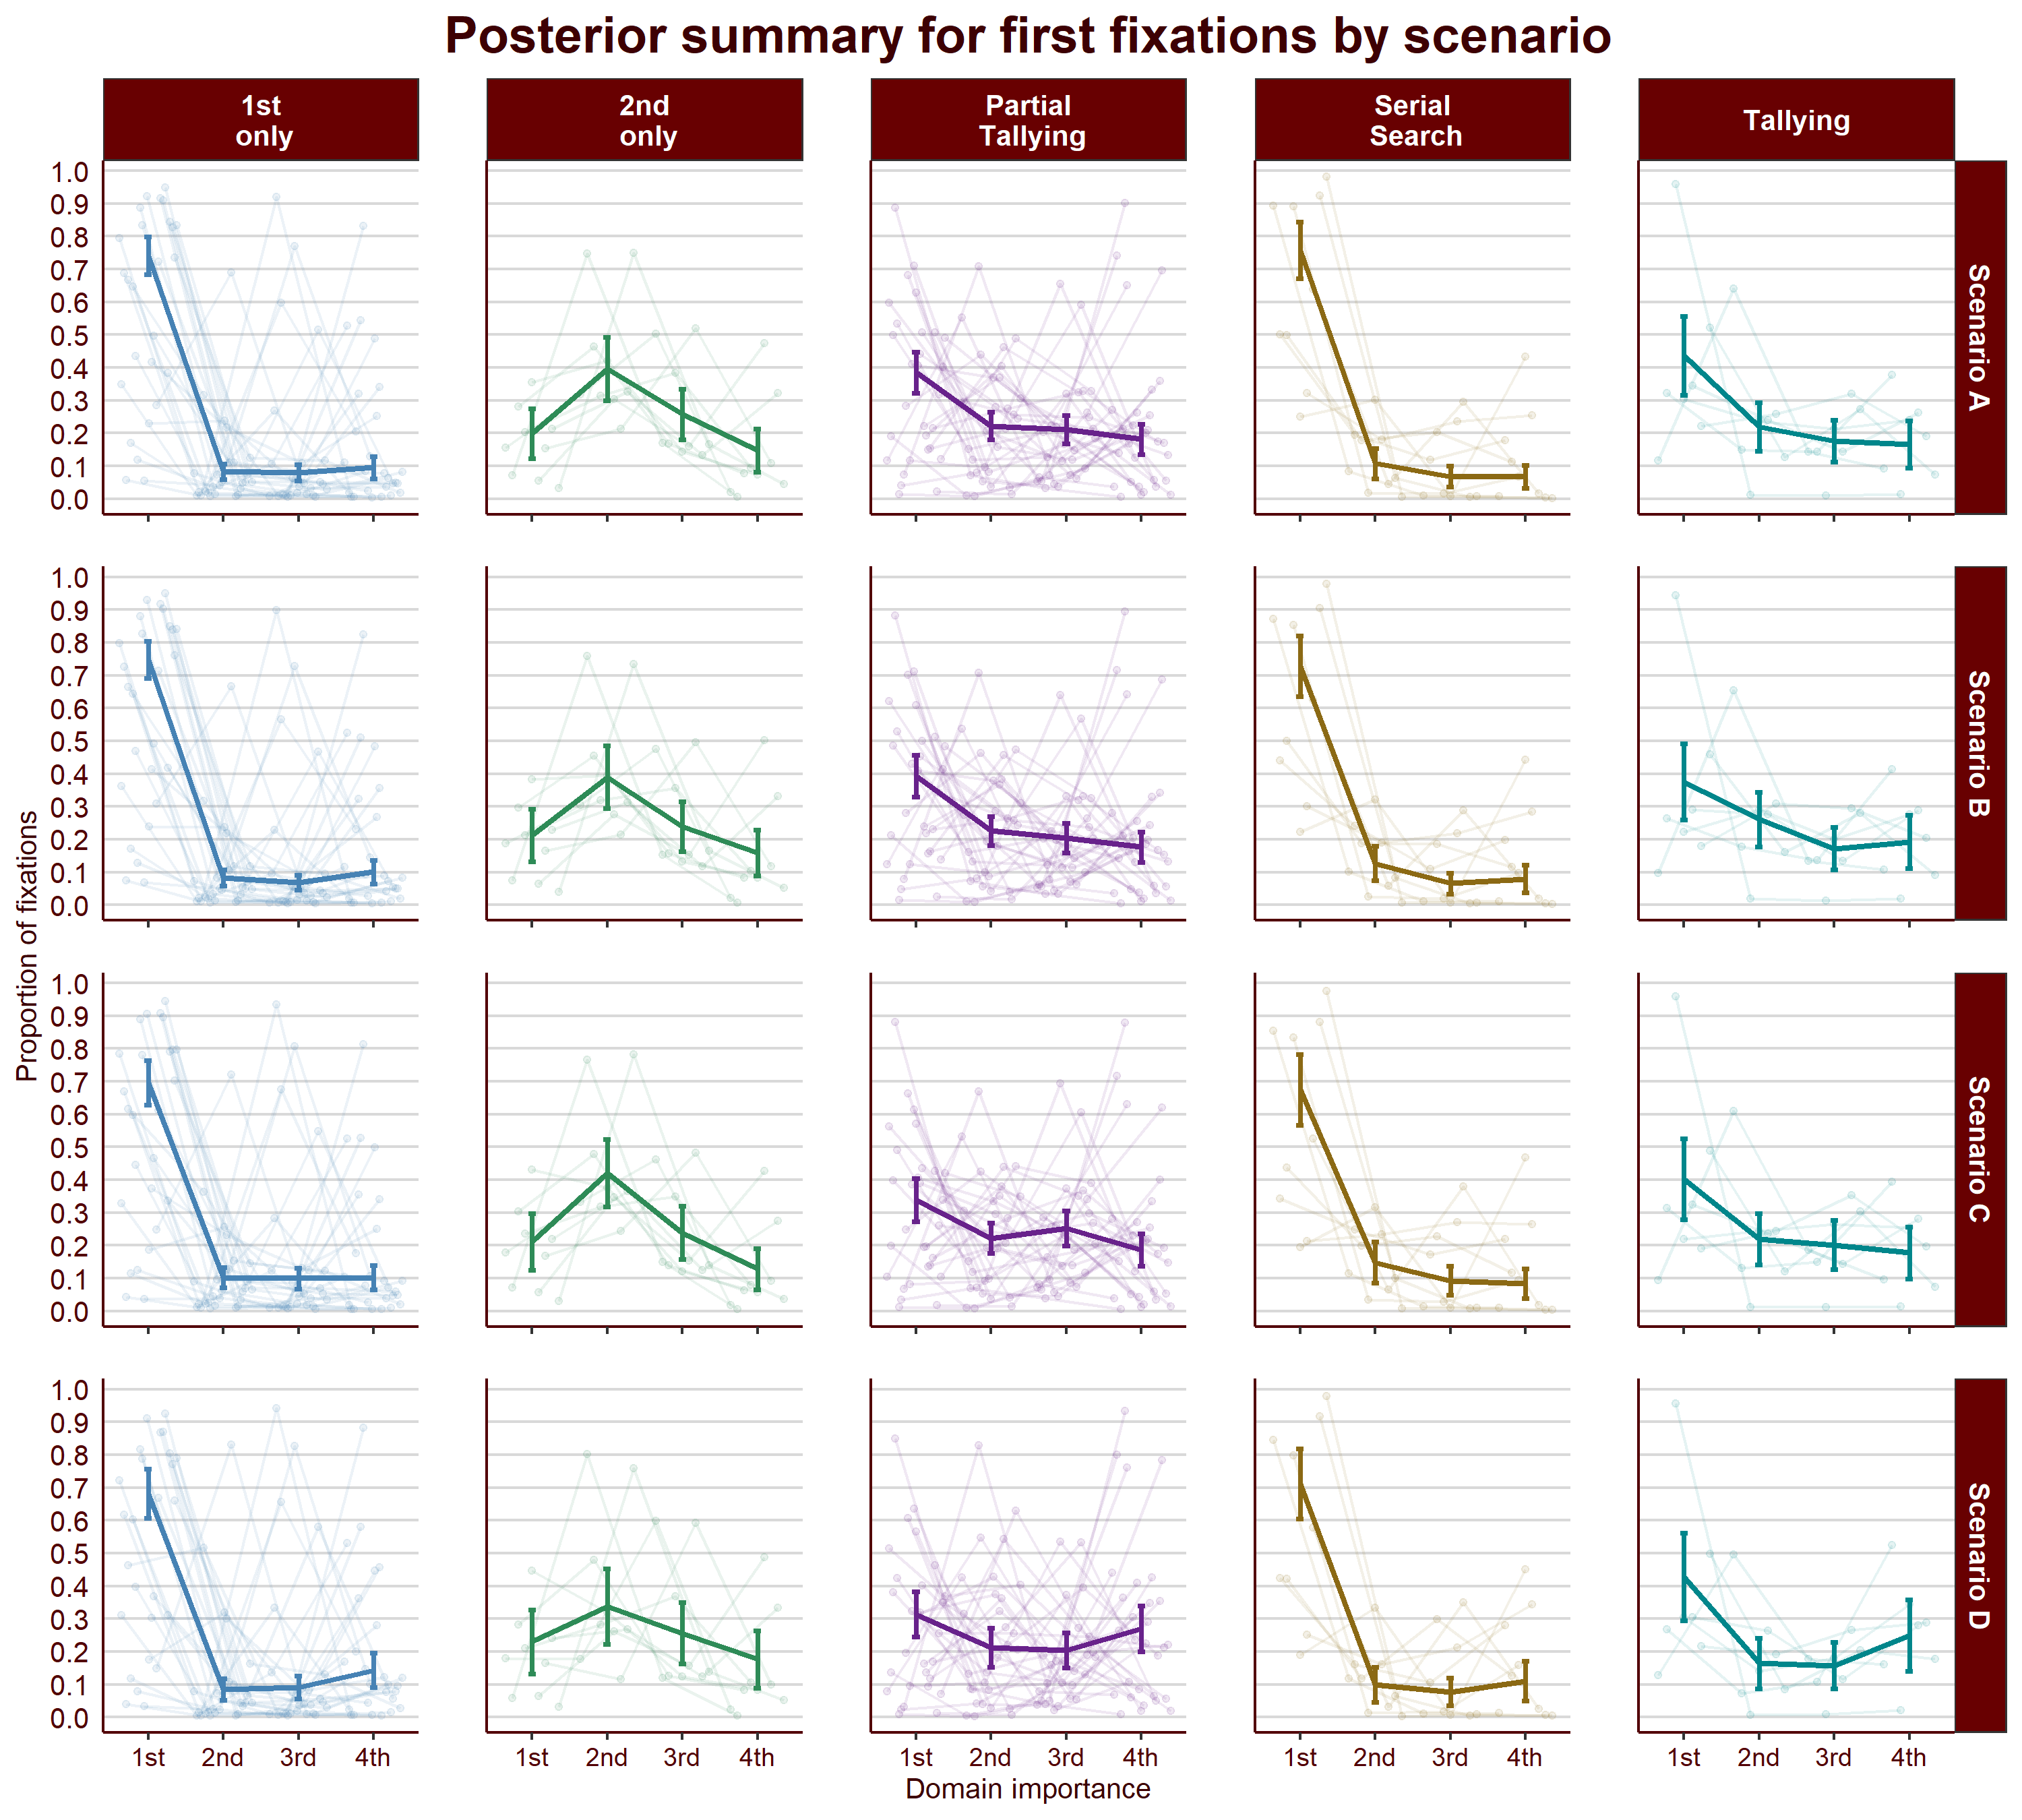
\includegraphics{C:/Users/rerr_/Google Drive/Graduate/Lab/Studies/MultiCue_Probabilistic/Stages/Shifted Weights/Eye Tracking/Analysis/Figures/C2_first_scenario.png}
\caption{\label{fig:first-scenario}Allocation of first fixations across domains in the different decision scenarios in T1. Individual dots correspond to the median from the posterior draws from each participant. Error bars represent standard deviations.}
\end{figure}

\begin{center}
\begin{ThreePartTable}

\begin{longtable}{llllll}\noalign{\getlongtablewidth\global\LTcapwidth=\longtablewidth}
\caption{\label{tab:table-first}Follow up comparisons for the proportion of first fixations across decision scenarios.}\\
\toprule
strategy & \multicolumn{1}{c}{comparison} & \multicolumn{1}{c}{ROPE\_Percentage} & \multicolumn{1}{c}{rawdirection} & \multicolumn{1}{c}{p\_HDI} & \multicolumn{1}{c}{p\_direction}\\
\midrule
\endfirsthead
\caption*{\normalfont{Table \ref{tab:table-first} continued}}\\
\toprule
strategy & \multicolumn{1}{c}{comparison} & \multicolumn{1}{c}{ROPE\_Percentage} & \multicolumn{1}{c}{rawdirection} & \multicolumn{1}{c}{p\_HDI} & \multicolumn{1}{c}{p\_direction}\\
\midrule
\endhead
1st only & d1\_all & 0.00 & 1.00 & 0.00\% & > 0.999\\
2nd only & d2\_all & 0.00 & 1.00 & 0.00\% & = 0.995\\
Partial Tallying & d1\_2 & 0.08 & 0.94 & 8.20\% & = 0.945\\
Partial Tallying & d12\_34 & 0.09 & 0.95 & 9.10\% & = 0.95\\
Partial Tallying & d3\_4 & 0.34 & 0.65 & 33.70\% & = 0.653\\
Serial Search & d1\_all & 0.00 & 1.00 & 0.00\% & > 0.999\\
Tallying & d1\_2 & 0.09 & 0.89 & 9.30\% & = 0.894\\
Tallying & d1\_3 & 0.04 & 0.94 & 3.90\% & = 0.944\\
Tallying & d1\_4 & 0.04 & 0.94 & 3.90\% & = 0.936\\
Tallying & d2\_3 & 0.26 & 0.70 & 25.50\% & = 0.696\\
Tallying & d2\_4 & 0.22 & 0.70 & 21.80\% & = 0.695\\
Tallying & d3\_4 & 0.27 & 0.53 & 26.70\% & = 0.533\\
\bottomrule
\end{longtable}

\end{ThreePartTable}
\end{center}

\begin{center}
\begin{ThreePartTable}

\begin{longtable}{lllllll}\noalign{\getlongtablewidth\global\LTcapwidth=\longtablewidth}
\caption{\label{tab:table-first-scenario}Follow up comparisons for the proportion of first fixations.}\\
\toprule
strategy & \multicolumn{1}{c}{scenario} & \multicolumn{1}{c}{comparison} & \multicolumn{1}{c}{ROPE\_Percentage} & \multicolumn{1}{c}{rawdirection} & \multicolumn{1}{c}{p\_HDI} & \multicolumn{1}{c}{p\_direction}\\
\midrule
\endfirsthead
\caption*{\normalfont{Table \ref{tab:table-first-scenario} continued}}\\
\toprule
strategy & \multicolumn{1}{c}{scenario} & \multicolumn{1}{c}{comparison} & \multicolumn{1}{c}{ROPE\_Percentage} & \multicolumn{1}{c}{rawdirection} & \multicolumn{1}{c}{p\_HDI} & \multicolumn{1}{c}{p\_direction}\\
\midrule
\endhead
1st only & 0 & d1\_all & 0.00 & 1.00 & 0.000\% & > 0.999\\
1st only & 1 & d1\_all & 0.00 & 1.00 & 0.000\% & > 0.999\\
1st only & 2 & d1\_all & 0.00 & 1.00 & 0.000\% & > 0.999\\
1st only & 3 & d1\_all & 0.00 & 1.00 & 0.000\% & > 0.999\\
2nd only & 0 & d2\_all & 0.00 & 1.00 & 0.000\% & = 0.996\\
2nd only & 1 & d2\_all & 0.00 & 1.00 & 0.000\% & = 0.995\\
2nd only & 2 & d2\_all & 0.00 & 1.00 & 0.000\% & = 0.997\\
2nd only & 3 & d2\_all & 0.07 & 0.93 & 7.000\% & = 0.932\\
Partial Tallying & 0 & d1\_2 & 0.03 & 0.96 & 3.200\% & = 0.965\\
Partial Tallying & 0 & d12\_34 & 0.07 & 0.96 & 7.200\% & = 0.959\\
Partial Tallying & 0 & d3\_4 & 0.33 & 0.68 & 33.200\% & = 0.675\\
Partial Tallying & 1 & d1\_2 & 0.04 & 0.96 & 3.700\% & = 0.965\\
Partial Tallying & 1 & d12\_34 & 0.03 & 0.97 & 3.000\% & = 0.973\\
Partial Tallying & 1 & d3\_4 & 0.33 & 0.66 & 32.800\% & = 0.665\\
Partial Tallying & 2 & d1\_2 & 0.16 & 0.90 & 16.200\% & = 0.897\\
Partial Tallying & 2 & d12\_34 & 0.29 & 0.83 & 29.100\% & = 0.831\\
Partial Tallying & 2 & d3\_4 & 0.23 & 0.80 & 23.300\% & = 0.801\\
Partial Tallying & 3 & d1\_2 & 0.18 & 0.83 & 18.200\% & = 0.834\\
Partial Tallying & 3 & d12\_34 & 0.36 & 0.63 & 36.400\% & = 0.633\\
Partial Tallying & 3 & d3\_4 & 0.23 & 0.74 & 22.800\% & = 0.745\\
Serial Search & 0 & d1\_all & 0.00 & 1.00 & 0.000\% & > 0.999\\
Serial Search & 1 & d1\_all & 0.00 & 1.00 & 0.000\% & > 0.999\\
Serial Search & 2 & d1\_all & 0.00 & 1.00 & 0.000\% & > 0.999\\
Serial Search & 3 & d1\_all & 0.00 & 1.00 & 0.000\% & > 0.999\\
Tallying & 0 & d1\_2 & 0.09 & 0.89 & 9.400\% & = 0.89\\
Tallying & 0 & d1\_3 & 0.04 & 0.94 & 4.500\% & = 0.941\\
Tallying & 0 & d1\_4 & 0.03 & 0.94 & 2.900\% & = 0.941\\
Tallying & 0 & d2\_3 & 0.25 & 0.70 & 24.800\% & = 0.698\\
Tallying & 0 & d2\_4 & 0.20 & 0.72 & 20.100\% & = 0.725\\
Tallying & 0 & d3\_4 & 0.25 & 0.57 & 25.300\% & = 0.568\\
Tallying & 1 & d1\_2 & 0.16 & 0.74 & 15.700\% & = 0.737\\
Tallying & 1 & d1\_3 & 0.08 & 0.91 & 8.100\% & = 0.909\\
Tallying & 1 & d1\_4 & 0.10 & 0.86 & 9.900\% & = 0.86\\
Tallying & 1 & d2\_3 & 0.18 & 0.82 & 17.800\% & = 0.815\\
Tallying & 1 & d2\_4 & 0.19 & 0.73 & 18.600\% & = 0.733\\
Tallying & 1 & d3\_4 & 0.24 & 0.56 & 24.100\% & = 0.563\\
Tallying & 2 & d1\_2 & 0.11 & 0.85 & 11.100\% & = 0.847\\
Tallying & 2 & d1\_3 & 0.10 & 0.88 & 9.800\% & = 0.875\\
Tallying & 2 & d1\_4 & 0.07 & 0.90 & 7.400\% & = 0.898\\
Tallying & 2 & d2\_3 & 0.25 & 0.57 & 24.700\% & = 0.569\\
Tallying & 2 & d2\_4 & 0.20 & 0.67 & 20.100\% & = 0.669\\
Tallying & 2 & d3\_4 & 0.22 & 0.61 & 21.900\% & = 0.613\\
Tallying & 3 & d1\_2 & 0.06 & 0.93 & 5.900\% & = 0.928\\
Tallying & 3 & d1\_3 & 0.05 & 0.94 & 5.200\% & = 0.939\\
Tallying & 3 & d1\_4 & 0.11 & 0.79 & 10.800\% & = 0.793\\
Tallying & 3 & d2\_3 & 0.22 & 0.52 & 21.600\% & = 0.523\\
Tallying & 3 & d2\_4 & 0.16 & 0.73 & 16.000\% & = 0.731\\
Tallying & 3 & d3\_4 & 0.16 & 0.76 & 15.700\% & = 0.762\\
\bottomrule
\end{longtable}

\end{ThreePartTable}
\end{center}

\begin{figure}
\centering
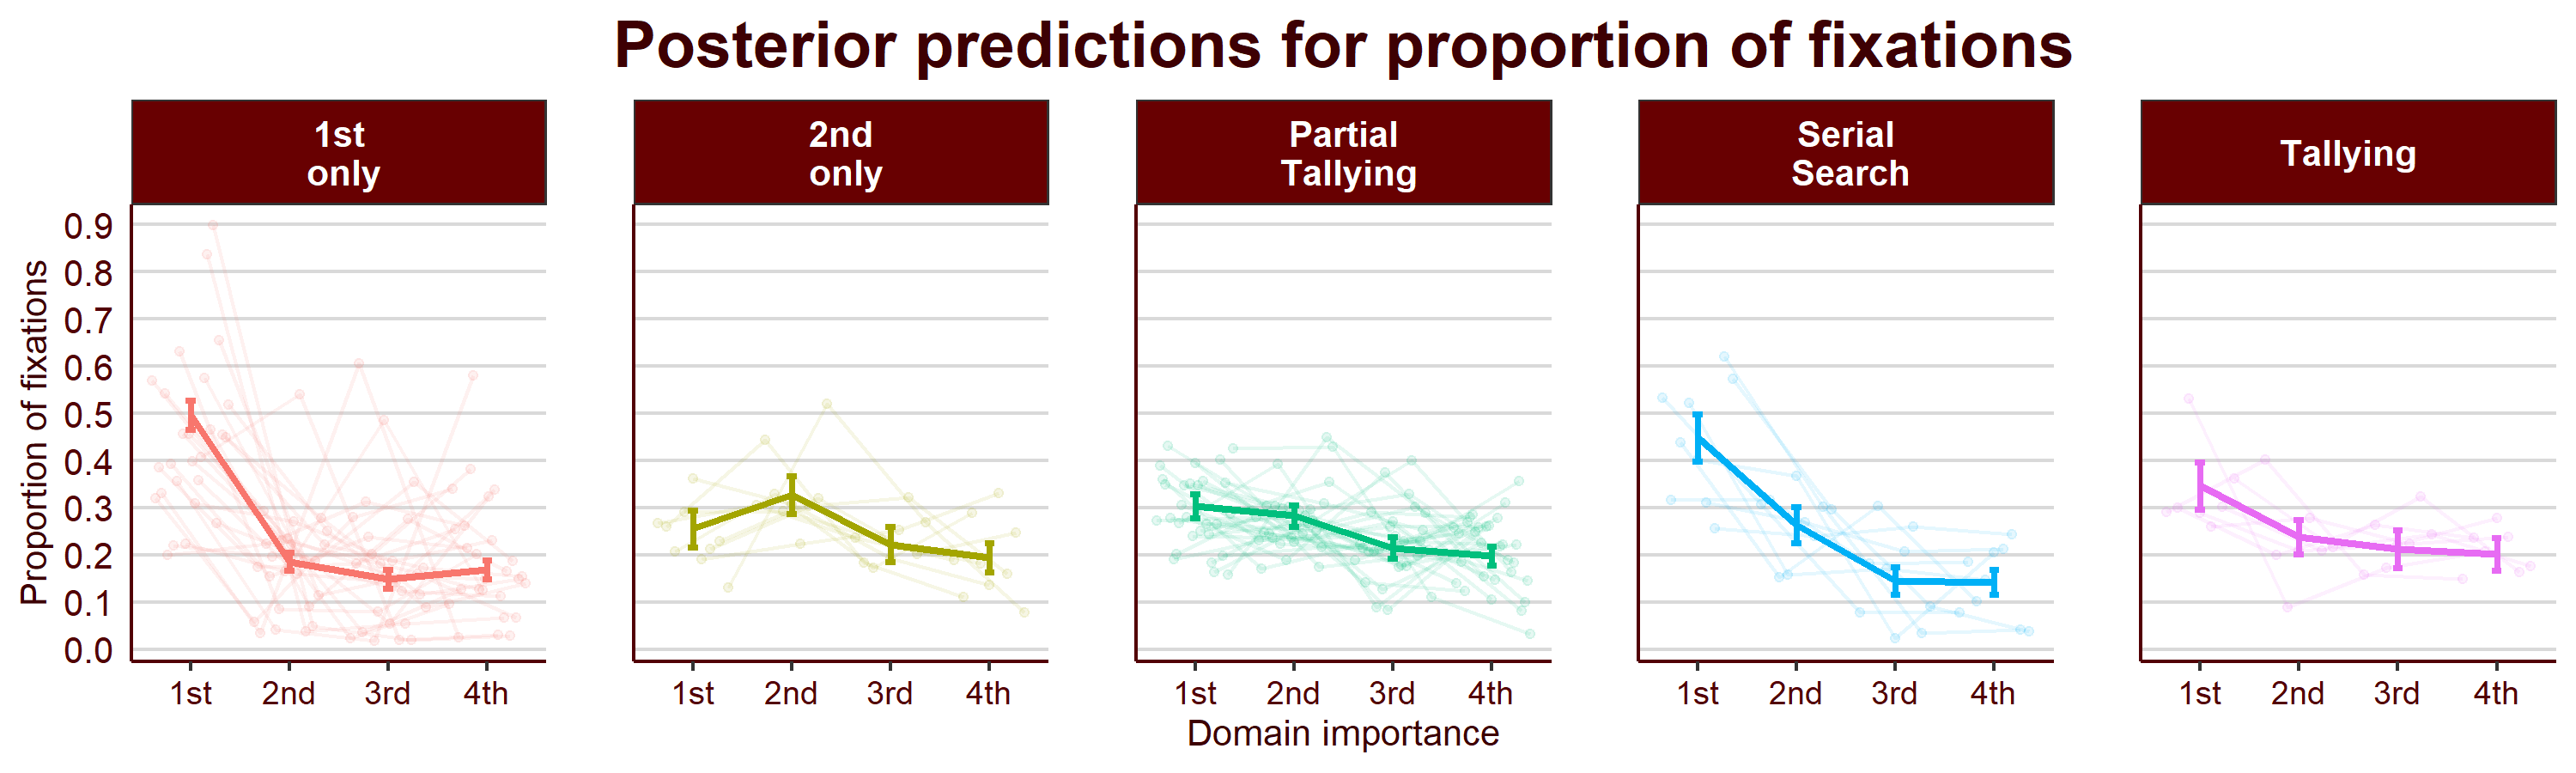
\includegraphics{C:/Users/rerr_/Google Drive/Graduate/Lab/Studies/MultiCue_Probabilistic/Stages/Shifted Weights/Eye Tracking/Analysis/Figures/D1_proportion.png}
\caption{\label{fig:proportion}Allocation of fixations across domains in T1 for the different decision groups. Individual dots correspond to the median from the posterior draws from each participant. Error bars represent standard deviations.}
\end{figure}

\begin{figure}
\centering
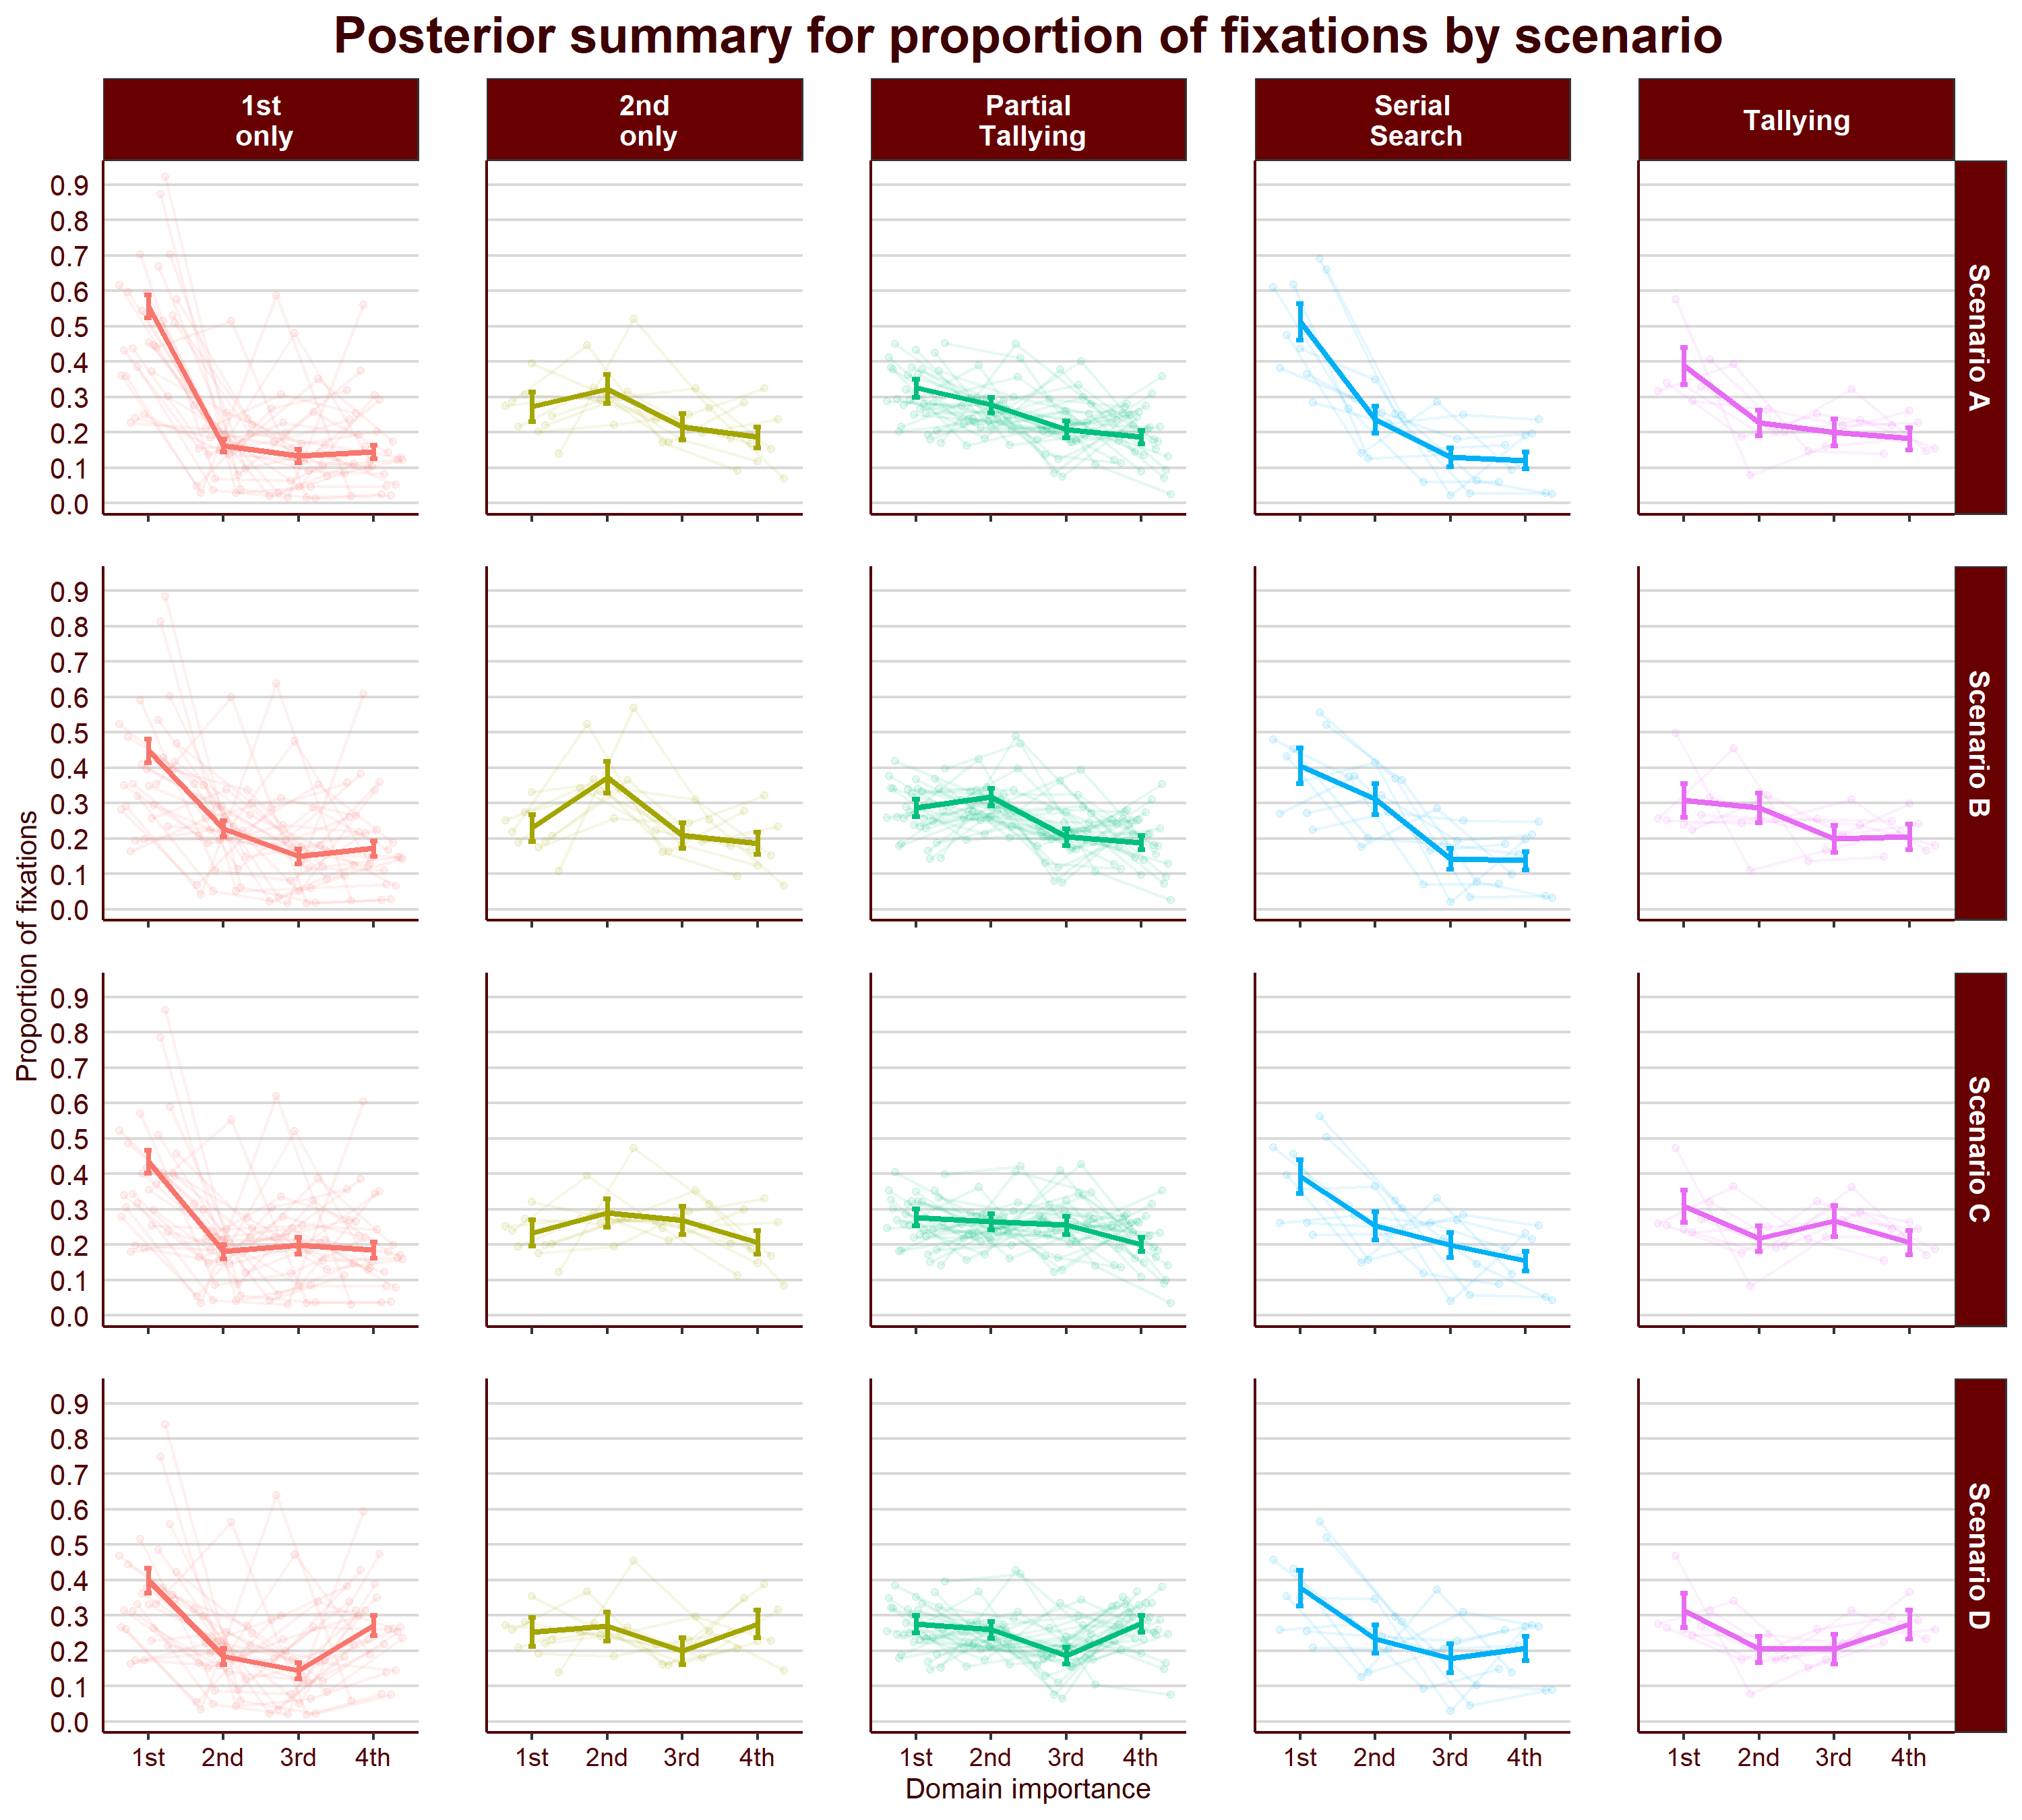
\includegraphics{C:/Users/rerr_/Google Drive/Graduate/Lab/Studies/MultiCue_Probabilistic/Stages/Shifted Weights/Eye Tracking/Analysis/Figures/D2_proportion_scenario.png}
\caption{\label{fig:proportion-scenario}Allocation of fixations across domains in T1 for the different decision groups. Individual dots correspond to the median from the posterior draws from each participant. Error bars represent standard deviations.}
\end{figure}

\begin{center}
\begin{ThreePartTable}

\begin{longtable}{llllll}\noalign{\getlongtablewidth\global\LTcapwidth=\longtablewidth}
\caption{\label{tab:table-proportion}Follow up comparisons for the proportion of fixations.}\\
\toprule
strategy & \multicolumn{1}{c}{comparison} & \multicolumn{1}{c}{ROPE\_Percentage} & \multicolumn{1}{c}{rawdirection} & \multicolumn{1}{c}{p\_HDI} & \multicolumn{1}{c}{p\_direction}\\
\midrule
\endfirsthead
\caption*{\normalfont{Table \ref{tab:table-proportion} continued}}\\
\toprule
strategy & \multicolumn{1}{c}{comparison} & \multicolumn{1}{c}{ROPE\_Percentage} & \multicolumn{1}{c}{rawdirection} & \multicolumn{1}{c}{p\_HDI} & \multicolumn{1}{c}{p\_direction}\\
\midrule
\endhead
1st only & d1\_all & 0.00 & 1.00 & 0.00\% & > 0.999\\
2nd only & d2\_all & 0.00 & 1.00 & 0.00\% & > 0.999\\
Partial Tallying & d1\_2 & 0.68 & 0.70 & 67.90\% & = 0.703\\
Partial Tallying & d12\_34 & 0.00 & 1.00 & 0.00\% & = 0.999\\
Partial Tallying & d3\_4 & 0.65 & 0.69 & 64.60\% & = 0.69\\
Serial Search & d1\_2 & 0.00 & 0.99 & 0.00\% & = 0.988\\
Serial Search & d2\_3 & 0.00 & 0.99 & 0.00\% & = 0.994\\
Serial Search & d3\_4 & 0.52 & 0.53 & 52.50\% & = 0.531\\
Serial Search & lin1 & 0.27 & 0.56 & 26.70\% & = 0.562\\
Serial Search & lin2 & 0.13 & 0.91 & 13.20\% & = 0.909\\
Serial Search & lin3 & 0.14 & 0.72 & 14.10\% & = 0.72\\
Tallying & d1\_2 & 0.12 & 0.93 & 12.00\% & = 0.933\\
Tallying & d1\_3 & 0.05 & 0.96 & 4.80\% & = 0.957\\
Tallying & d1\_4 & 0.01 & 0.98 & 1.30\% & = 0.977\\
Tallying & d2\_3 & 0.38 & 0.70 & 37.60\% & = 0.698\\
Tallying & d2\_4 & 0.37 & 0.76 & 37.20\% & = 0.757\\
Tallying & d3\_4 & 0.50 & 0.56 & 49.50\% & = 0.562\\
\bottomrule
\end{longtable}

\end{ThreePartTable}
\end{center}

\begin{center}
\begin{ThreePartTable}

\begin{longtable}{lllllll}\noalign{\getlongtablewidth\global\LTcapwidth=\longtablewidth}
\caption{\label{tab:table-proportion-scenario}Follow up comparisons for the proportion of fixations across decision scenarios.}\\
\toprule
strategy & \multicolumn{1}{c}{scenario} & \multicolumn{1}{c}{comparison} & \multicolumn{1}{c}{ROPE\_Percentage} & \multicolumn{1}{c}{rawdirection} & \multicolumn{1}{c}{p\_HDI} & \multicolumn{1}{c}{p\_direction}\\
\midrule
\endfirsthead
\caption*{\normalfont{Table \ref{tab:table-proportion-scenario} continued}}\\
\toprule
strategy & \multicolumn{1}{c}{scenario} & \multicolumn{1}{c}{comparison} & \multicolumn{1}{c}{ROPE\_Percentage} & \multicolumn{1}{c}{rawdirection} & \multicolumn{1}{c}{p\_HDI} & \multicolumn{1}{c}{p\_direction}\\
\midrule
\endhead
1st only & 0 & d1\_all & 0.00 & 1.00 & 0.000\% & > 0.999\\
1st only & 1 & d1\_all & 0.00 & 1.00 & 0.000\% & > 0.999\\
1st only & 2 & d1\_all & 0.00 & 1.00 & 0.000\% & > 0.999\\
1st only & 3 & d1\_all & 0.00 & 1.00 & 0.000\% & > 0.999\\
2nd only & 0 & d2\_all & 0.00 & 1.00 & 0.000\% & = 0.998\\
2nd only & 1 & d2\_all & 0.00 & 1.00 & 0.000\% & > 0.999\\
2nd only & 2 & d2\_all & 0.08 & 0.98 & 8.000\% & = 0.981\\
2nd only & 3 & d2\_all & 0.26 & 0.93 & 25.800\% & = 0.931\\
Partial Tallying & 0 & d1\_2 & 0.41 & 0.88 & 41.000\% & = 0.882\\
Partial Tallying & 0 & d12\_34 & 0.00 & 1.00 & 0.000\% & > 0.999\\
Partial Tallying & 0 & d3\_4 & 0.59 & 0.74 & 58.900\% & = 0.735\\
Partial Tallying & 1 & d1\_2 & 0.57 & 0.77 & 57.400\% & = 0.77\\
Partial Tallying & 1 & d12\_34 & 0.00 & 1.00 & 0.000\% & > 0.999\\
Partial Tallying & 1 & d3\_4 & 0.63 & 0.67 & 62.600\% & = 0.667\\
Partial Tallying & 2 & d1\_2 & 0.72 & 0.62 & 71.800\% & = 0.625\\
Partial Tallying & 2 & d12\_34 & 0.32 & 0.95 & 32.400\% & = 0.948\\
Partial Tallying & 2 & d3\_4 & 0.26 & 0.93 & 25.800\% & = 0.93\\
Partial Tallying & 3 & d1\_2 & 0.65 & 0.65 & 65.100\% & = 0.652\\
Partial Tallying & 3 & d12\_34 & 0.40 & 0.92 & 40.200\% & = 0.917\\
Partial Tallying & 3 & d3\_4 & 0.02 & 0.99 & 1.600\% & = 0.99\\
Serial Search & 0 & d1\_all & 0.00 & 1.00 & 0.000\% & > 0.999\\
Serial Search & 1 & d1\_2 & 0.23 & 0.87 & 23.100\% & = 0.866\\
Serial Search & 1 & d12\_34 & 0.00 & 1.00 & 0.000\% & > 0.999\\
Serial Search & 2 & d1\_2 & 0.04 & 0.96 & 4.100\% & = 0.963\\
Serial Search & 2 & d1\_3 & 0.00 & 1.00 & 0.000\% & = 0.995\\
Serial Search & 2 & d2\_3 & 0.34 & 0.81 & 33.900\% & = 0.813\\
Serial Search & 2 & d3\_4 & 0.31 & 0.84 & 31.000\% & = 0.844\\
Serial Search & 3 & d1\_2 & 0.03 & 0.97 & 3.000\% & = 0.968\\
Serial Search & 3 & d1\_3 & 0.00 & 0.99 & 0.000\% & = 0.993\\
Serial Search & 3 & d2\_3 & 0.28 & 0.80 & 28.400\% & = 0.801\\
Serial Search & 3 & d3\_4 & 0.36 & 0.71 & 36.300\% & = 0.709\\
Tallying & 0 & d1\_2 & 0.01 & 0.98 & 0.700\% & = 0.982\\
Tallying & 0 & d1\_3 & 0.00 & 0.99 & 0.000\% & = 0.989\\
Tallying & 0 & d1\_4 & 0.00 & 1.00 & 0.000\% & = 0.997\\
Tallying & 0 & d2\_3 & 0.39 & 0.69 & 38.600\% & = 0.694\\
Tallying & 0 & d2\_4 & 0.32 & 0.82 & 31.900\% & = 0.816\\
Tallying & 0 & d3\_4 & 0.48 & 0.64 & 48.200\% & = 0.641\\
Tallying & 1 & d1\_2 & 0.42 & 0.61 & 42.000\% & = 0.612\\
Tallying & 1 & d1\_3 & 0.10 & 0.94 & 9.900\% & = 0.936\\
Tallying & 1 & d1\_4 & 0.11 & 0.93 & 11.300\% & = 0.931\\
Tallying & 1 & d2\_3 & 0.15 & 0.90 & 15.300\% & = 0.904\\
Tallying & 1 & d2\_4 & 0.17 & 0.90 & 17.000\% & = 0.905\\
Tallying & 1 & d3\_4 & 0.47 & 0.55 & 47.300\% & = 0.553\\
Tallying & 2 & d1\_2 & 0.15 & 0.92 & 15.300\% & = 0.918\\
Tallying & 2 & d1\_3 & 0.35 & 0.71 & 35.400\% & = 0.711\\
Tallying & 2 & d1\_4 & 0.10 & 0.94 & 9.900\% & = 0.938\\
Tallying & 2 & d2\_3 & 0.36 & 0.78 & 35.900\% & = 0.784\\
Tallying & 2 & d2\_4 & 0.47 & 0.58 & 46.800\% & = 0.584\\
Tallying & 2 & d3\_4 & 0.29 & 0.85 & 29.100\% & = 0.85\\
Tallying & 3 & d1\_2 & 0.10 & 0.94 & 9.800\% & = 0.945\\
Tallying & 3 & d1\_3 & 0.12 & 0.92 & 11.700\% & = 0.922\\
Tallying & 3 & d1\_4 & 0.38 & 0.70 & 38.100\% & = 0.702\\
Tallying & 3 & d2\_3 & 0.41 & 0.52 & 40.700\% & = 0.516\\
Tallying & 3 & d2\_4 & 0.24 & 0.88 & 23.500\% & = 0.879\\
Tallying & 3 & d3\_4 & 0.22 & 0.87 & 22.500\% & = 0.866\\
\bottomrule
\end{longtable}

\end{ThreePartTable}
\end{center}

\begin{figure}
\centering
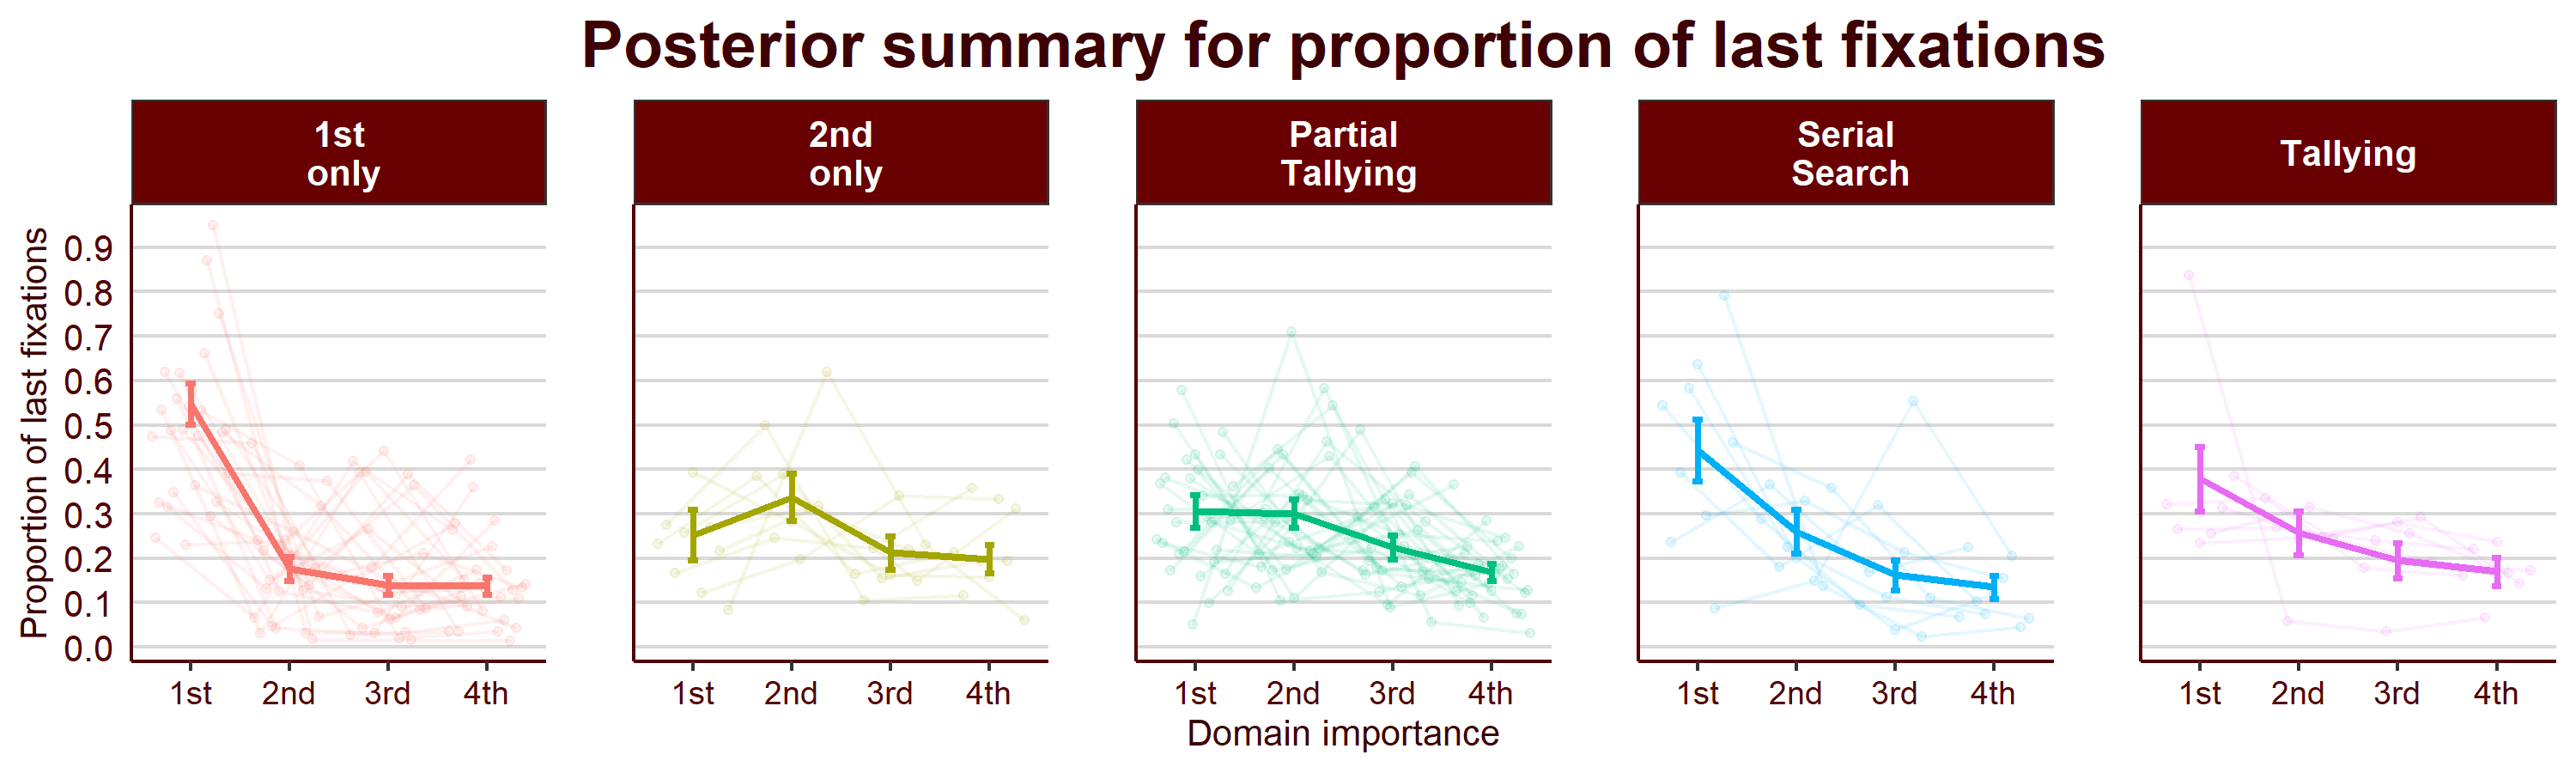
\includegraphics{C:/Users/rerr_/Google Drive/Graduate/Lab/Studies/MultiCue_Probabilistic/Stages/Shifted Weights/Eye Tracking/Analysis/Figures/E1_last.png}
\caption{\label{fig:last}Allocation of the last fixations across domains in T1. Individual dots correspond to the median from the posterior draws from each participant. Error bars represent standard deviations.}
\end{figure}

\begin{figure}
\centering
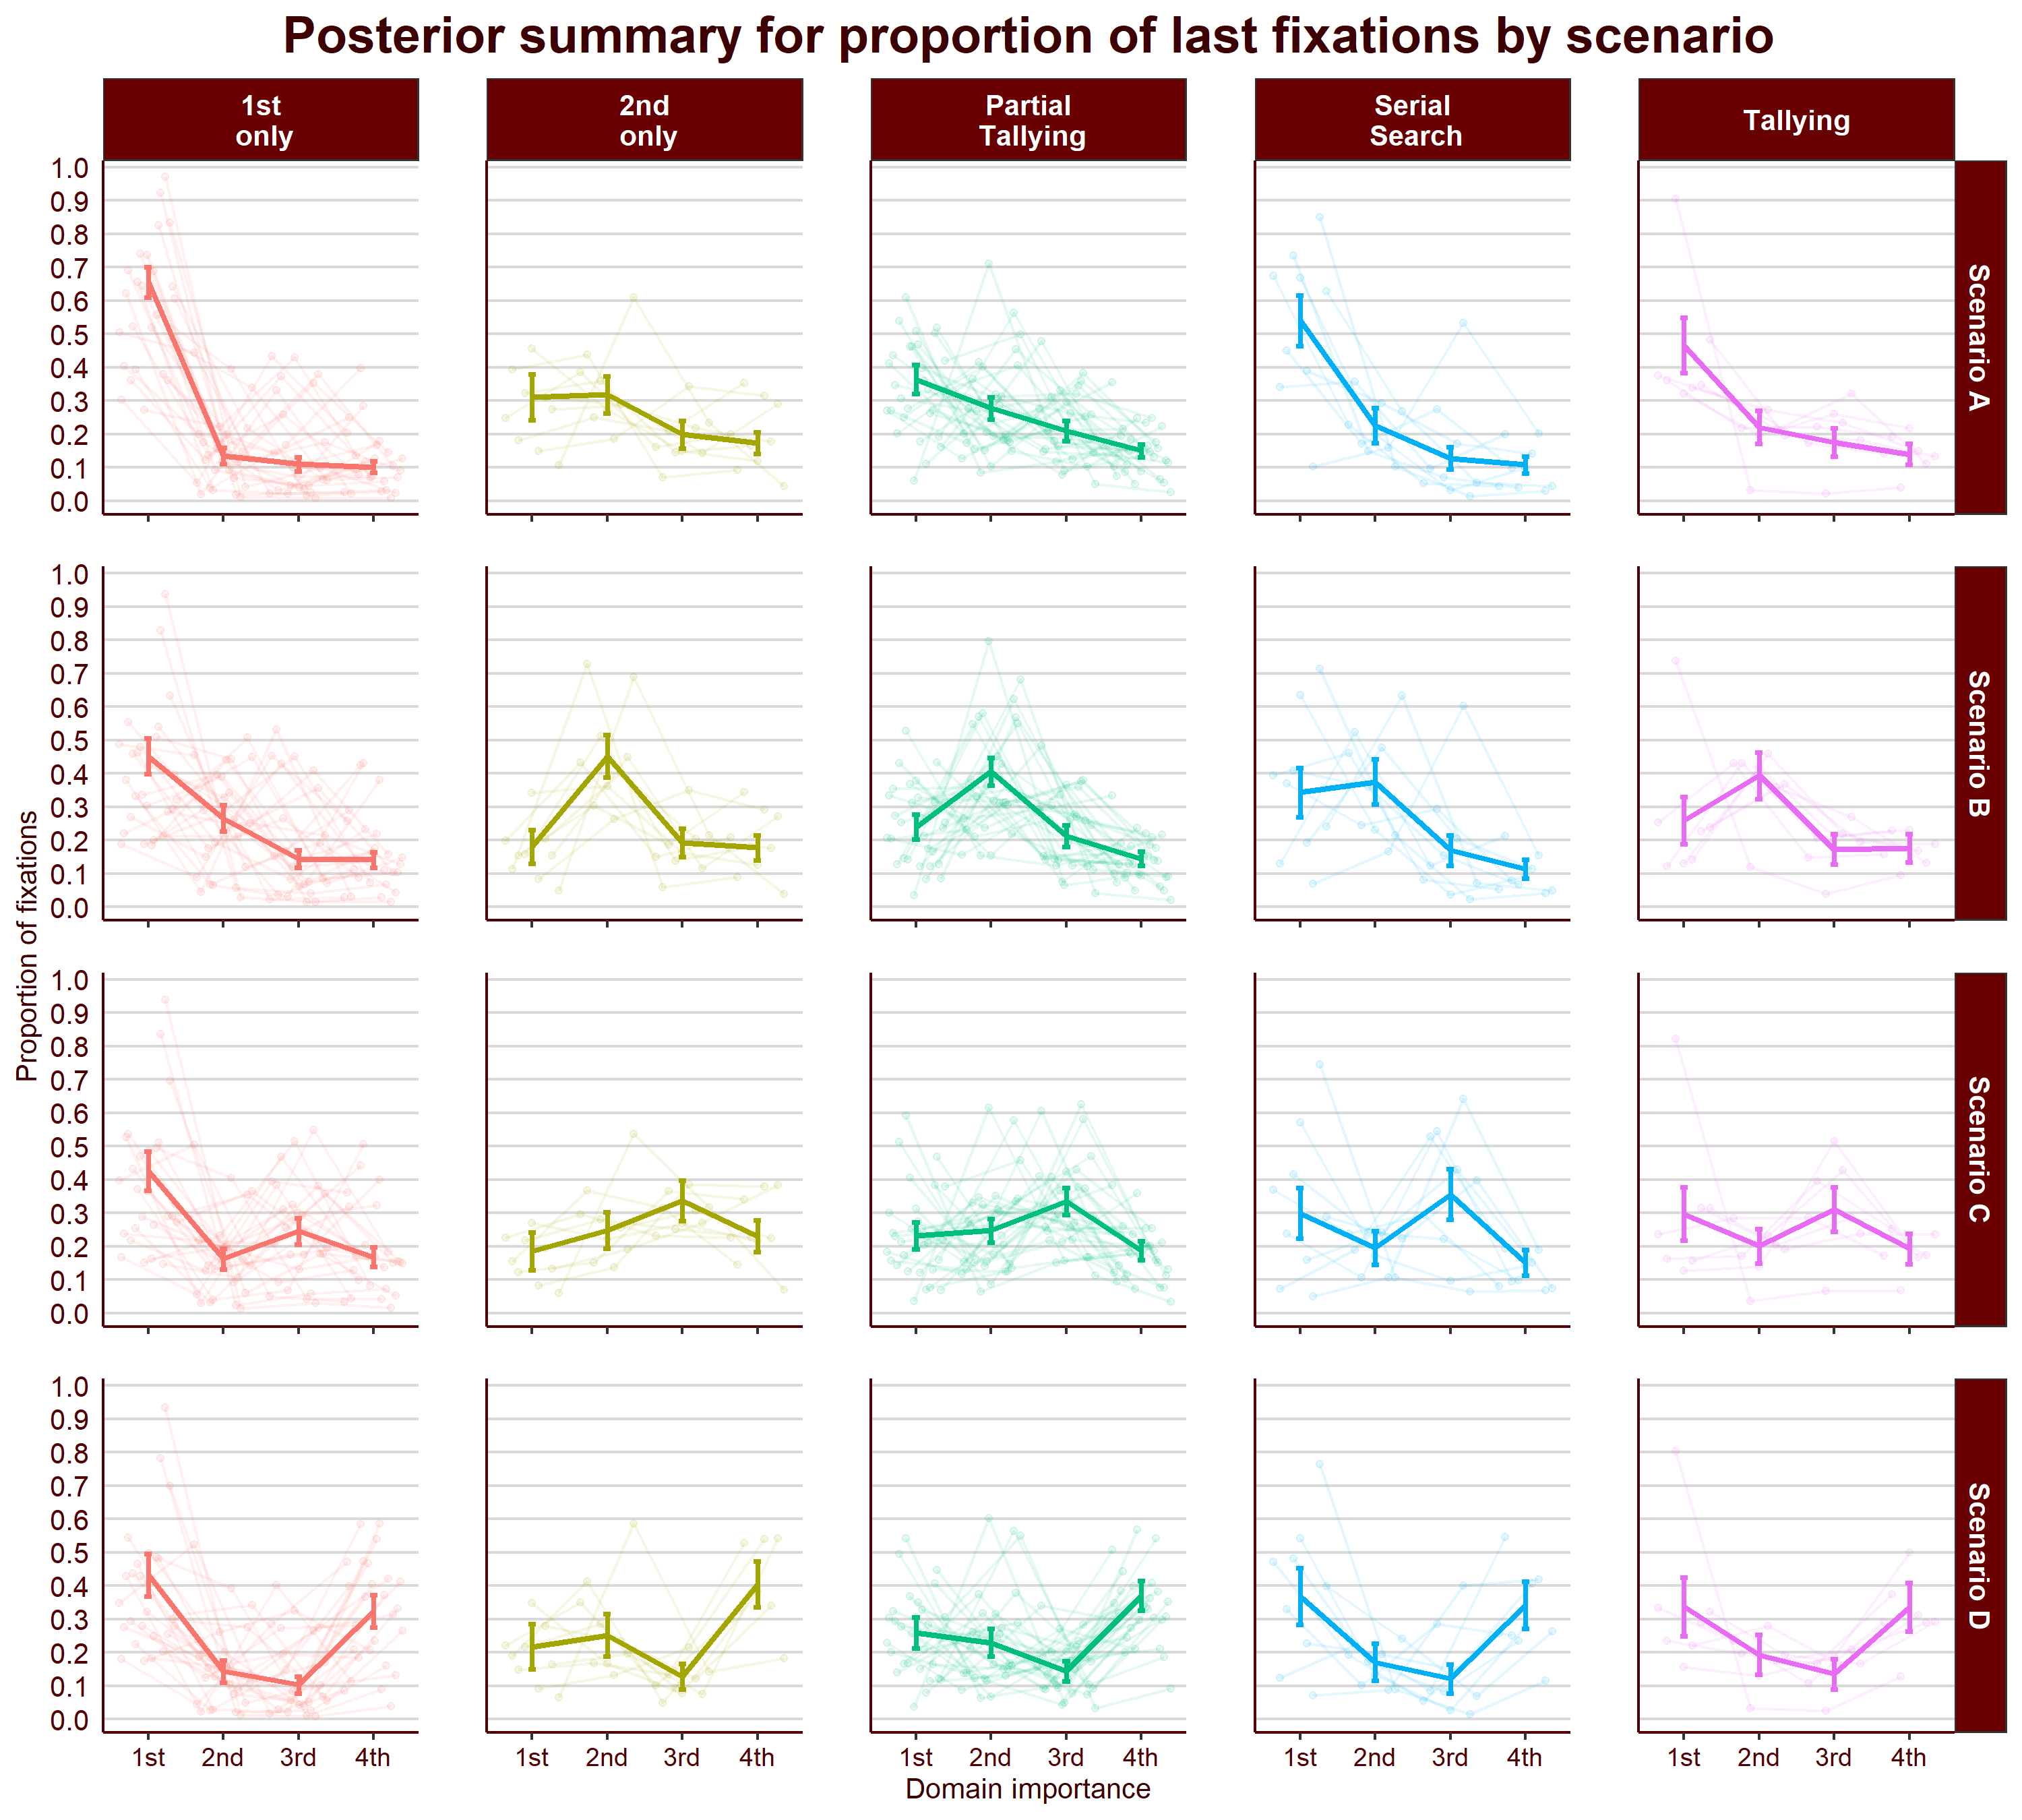
\includegraphics{C:/Users/rerr_/Google Drive/Graduate/Lab/Studies/MultiCue_Probabilistic/Stages/Shifted Weights/Eye Tracking/Analysis/Figures/E2_last_scenario.png}
\caption{\label{fig:last-scenario}Allocation of last fixations across domains in the different decision scenarios in T1. Individual dots correspond to the median from the posterior draws from each participant. Error bars represent standard deviations.}
\end{figure}

\begin{center}
\begin{ThreePartTable}

\begin{longtable}{llllll}\noalign{\getlongtablewidth\global\LTcapwidth=\longtablewidth}
\caption{\label{tab:table-last}Follow up comparisons for the last fixations.}\\
\toprule
strategy & \multicolumn{1}{c}{comparison} & \multicolumn{1}{c}{ROPE\_Percentage} & \multicolumn{1}{c}{rawdirection} & \multicolumn{1}{c}{p\_HDI} & \multicolumn{1}{c}{p\_direction}\\
\midrule
\endfirsthead
\caption*{\normalfont{Table \ref{tab:table-last} continued}}\\
\toprule
strategy & \multicolumn{1}{c}{comparison} & \multicolumn{1}{c}{ROPE\_Percentage} & \multicolumn{1}{c}{rawdirection} & \multicolumn{1}{c}{p\_HDI} & \multicolumn{1}{c}{p\_direction}\\
\midrule
\endhead
1st only & d1\_all & 0.00 & 1.00 & 0.00\% & > 0.999\\
2nd only & d2\_all & 0.02 & 0.99 & 1.90\% & = 0.988\\
Partial Tallying & d1\_2 & 0.54 & 0.53 & 54.10\% & = 0.534\\
Partial Tallying & d12\_34 & 0.00 & 1.00 & 0.00\% & > 0.999\\
Partial Tallying & d3\_4 & 0.18 & 0.96 & 18.50\% & = 0.959\\
Serial Search & d1\_2 & 0.05 & 0.95 & 5.00\% & = 0.947\\
Serial Search & d2\_3 & 0.06 & 0.97 & 6.10\% & = 0.968\\
Serial Search & d3\_4 & 0.43 & 0.77 & 42.70\% & = 0.771\\
Serial Search & lin1 & 0.21 & 0.64 & 20.80\% & = 0.638\\
Serial Search & lin2 & 0.24 & 0.77 & 23.60\% & = 0.767\\
Serial Search & lin3 & 0.15 & 0.54 & 14.60\% & = 0.54\\
Tallying & d1\_2 & 0.18 & 0.87 & 17.80\% & = 0.869\\
Tallying & d1\_3 & 0.01 & 0.97 & 1.30\% & = 0.968\\
Tallying & d1\_4 & 0.00 & 0.99 & 0.00\% & = 0.991\\
Tallying & d2\_3 & 0.25 & 0.85 & 24.80\% & = 0.849\\
Tallying & d2\_4 & 0.10 & 0.93 & 10.40\% & = 0.934\\
Tallying & d3\_4 & 0.44 & 0.71 & 43.90\% & = 0.714\\
\bottomrule
\end{longtable}

\end{ThreePartTable}
\end{center}

\begin{center}
\begin{ThreePartTable}

\begin{longtable}{lllllll}\noalign{\getlongtablewidth\global\LTcapwidth=\longtablewidth}
\caption{\label{tab:table-last-scenario}Follow up comparisons for the proportion of last fixations.}\\
\toprule
strategy & \multicolumn{1}{c}{scenario} & \multicolumn{1}{c}{comparison} & \multicolumn{1}{c}{ROPE\_Percentage} & \multicolumn{1}{c}{rawdirection} & \multicolumn{1}{c}{p\_HDI} & \multicolumn{1}{c}{p\_direction}\\
\midrule
\endfirsthead
\caption*{\normalfont{Table \ref{tab:table-last-scenario} continued}}\\
\toprule
strategy & \multicolumn{1}{c}{scenario} & \multicolumn{1}{c}{comparison} & \multicolumn{1}{c}{ROPE\_Percentage} & \multicolumn{1}{c}{rawdirection} & \multicolumn{1}{c}{p\_HDI} & \multicolumn{1}{c}{p\_direction}\\
\midrule
\endhead
1st only & 0 & d1\_all & 0.00 & 1.00 & 0.00\% & > 0.999\\
1st only & 1 & d1\_all & 0.00 & 1.00 & 0.00\% & > 0.999\\
1st only & 2 & d1\_all & 0.00 & 1.00 & 0.00\% & = 0.999\\
1st only & 3 & d1\_all & 0.00 & 1.00 & 0.00\% & = 0.999\\
2nd only & 0 & d2\_all & 0.03 & 0.98 & 2.80\% & = 0.98\\
2nd only & 1 & d2\_all & 0.00 & 1.00 & 0.00\% & > 0.999\\
2nd only & 2 & d2\_all & 0.45 & 0.73 & 44.90\% & = 0.726\\
2nd only & 3 & d2\_all & 0.41 & 0.70 & 40.80\% & = 0.705\\
Partial Tallying & 0 & d1\_2 & 0.22 & 0.90 & 21.70\% & = 0.898\\
Partial Tallying & 0 & d12\_34 & 0.00 & 1.00 & 0.00\% & > 0.999\\
Partial Tallying & 0 & d3\_4 & 0.14 & 0.96 & 14.00\% & = 0.962\\
Partial Tallying & 1 & d1\_2 & 0.00 & 0.99 & 0.00\% & = 0.989\\
Partial Tallying & 1 & d12\_34 & 0.00 & 1.00 & 0.00\% & > 0.999\\
Partial Tallying & 1 & d3\_4 & 0.09 & 0.96 & 9.10\% & = 0.963\\
Partial Tallying & 2 & d1\_2 & 0.43 & 0.61 & 42.90\% & = 0.606\\
Partial Tallying & 2 & d12\_34 & 0.60 & 0.64 & 60.10\% & = 0.642\\
Partial Tallying & 2 & d3\_4 & 0.00 & 1.00 & 0.00\% & = 0.997\\
Partial Tallying & 3 & d1\_2 & 0.37 & 0.65 & 37.20\% & = 0.652\\
Partial Tallying & 3 & d12\_34 & 0.57 & 0.54 & 56.70\% & = 0.537\\
Partial Tallying & 3 & d3\_4 & 0.00 & 1.00 & 0.00\% & > 0.999\\
Serial Search & 0 & d1\_all & 0.00 & 1.00 & 0.00\% & > 0.999\\
Serial Search & 1 & d2\_all & 0.00 & 1.00 & 0.00\% & = 0.997\\
Tallying & 0 & d1\_2 & 0.00 & 0.98 & 0.00\% & = 0.975\\
Tallying & 0 & d1\_3 & 0.00 & 0.99 & 0.00\% & = 0.993\\
Tallying & 0 & d1\_4 & 0.00 & 1.00 & 0.00\% & = 0.999\\
Tallying & 0 & d2\_3 & 0.29 & 0.79 & 28.60\% & = 0.79\\
Tallying & 0 & d2\_4 & 0.08 & 0.94 & 8.20\% & = 0.938\\
Tallying & 0 & d3\_4 & 0.36 & 0.80 & 35.80\% & = 0.8\\
Tallying & 1 & d1\_2 & 0.15 & 0.86 & 14.90\% & = 0.858\\
Tallying & 1 & d1\_3 & 0.19 & 0.82 & 18.80\% & = 0.825\\
Tallying & 1 & d1\_4 & 0.19 & 0.82 & 19.40\% & = 0.821\\
Tallying & 1 & d2\_3 & 0.00 & 0.99 & 0.00\% & = 0.988\\
Tallying & 1 & d2\_4 & 0.00 & 0.99 & 0.00\% & = 0.989\\
Tallying & 1 & d3\_4 & 0.38 & 0.52 & 37.50\% & = 0.518\\
Tallying & 2 & d1\_2 & 0.19 & 0.81 & 18.70\% & = 0.807\\
Tallying & 2 & d1\_3 & 0.25 & 0.56 & 24.70\% & = 0.559\\
Tallying & 2 & d1\_4 & 0.18 & 0.84 & 18.00\% & = 0.841\\
Tallying & 2 & d2\_3 & 0.16 & 0.89 & 15.60\% & = 0.889\\
Tallying & 2 & d2\_4 & 0.36 & 0.55 & 36.00\% & = 0.549\\
Tallying & 2 & d3\_4 & 0.10 & 0.92 & 10.30\% & = 0.919\\
Tallying & 3 & d1\_2 & 0.13 & 0.88 & 12.60\% & = 0.881\\
Tallying & 3 & d1\_3 & 0.01 & 0.97 & 1.30\% & = 0.969\\
Tallying & 3 & d1\_4 & 0.24 & 0.51 & 24.50\% & = 0.506\\
Tallying & 3 & d2\_3 & 0.20 & 0.79 & 20.30\% & = 0.794\\
Tallying & 3 & d2\_4 & 0.09 & 0.92 & 9.10\% & = 0.916\\
Tallying & 3 & d3\_4 & 0.00 & 0.98 & 0.00\% & = 0.985\\
\bottomrule
\end{longtable}

\end{ThreePartTable}
\end{center}


\clearpage
\renewcommand{\listfigurename}{Figure captions}

\clearpage
\renewcommand{\listtablename}{Table captions}


\clearpage
\makeatletter
\efloat@restorefloats
\makeatother


\begin{appendix}
\section{}
\renewcommand{\appendixname}{Supplementary Materials}
\renewcommand{\thefigure}{S\arabic{figure}} \setcounter{figure}{0}
\renewcommand{\thetable}{S\arabic{table}} \setcounter{table}{0}
\renewcommand{\theequation}{S\arabic{table}} \setcounter{equation}{0}
\graphicspath{{"../Documents/Tables and Figures/"}}

\begin{figure}
\centering
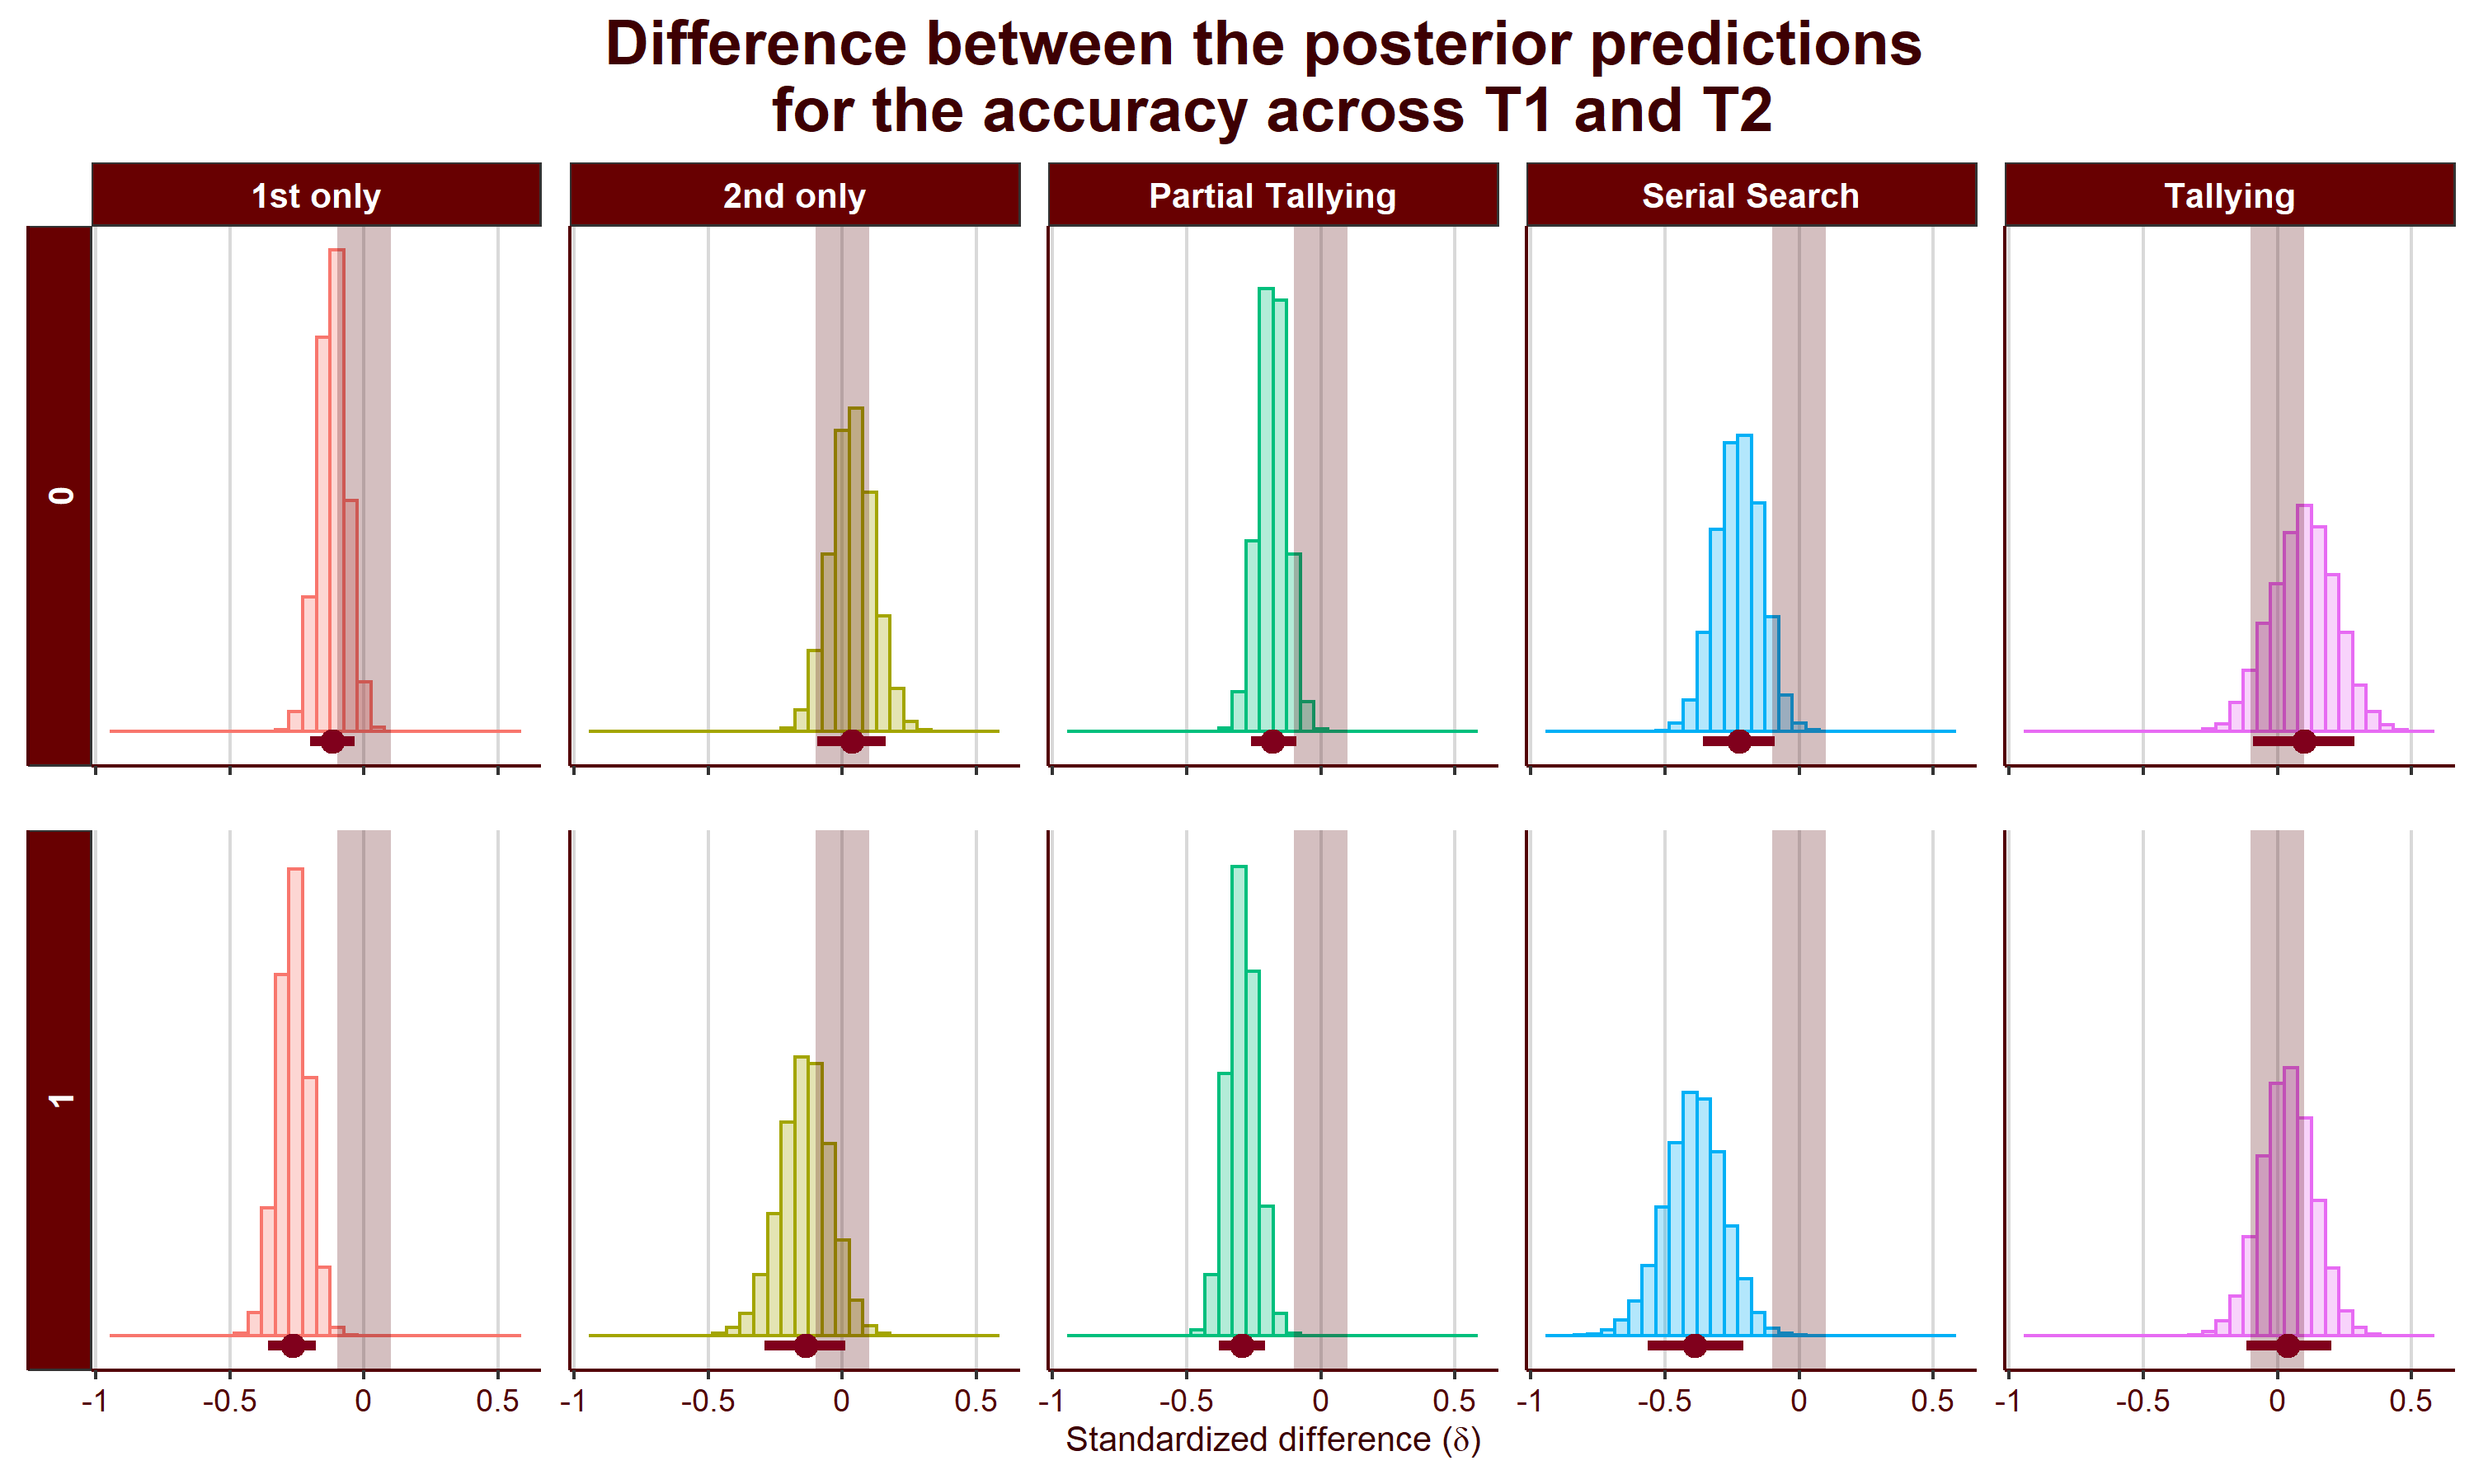
\includegraphics{C:/Users/rerr_/Google Drive/Graduate/Lab/Studies/MultiCue_Probabilistic/Stages/Shifted Weights/Eye Tracking/Analysis/Figures/SB1_performance_change.png}
\caption{\label{fig:performance-change}Difference in performance (as
standardized difference) across testing phases for the different
decision groups. The horizontal red bar represents the 0.89 HDI. The
shaded area highlights the ROPE used in these comparisons}
\end{figure}

\begin{figure}
\centering
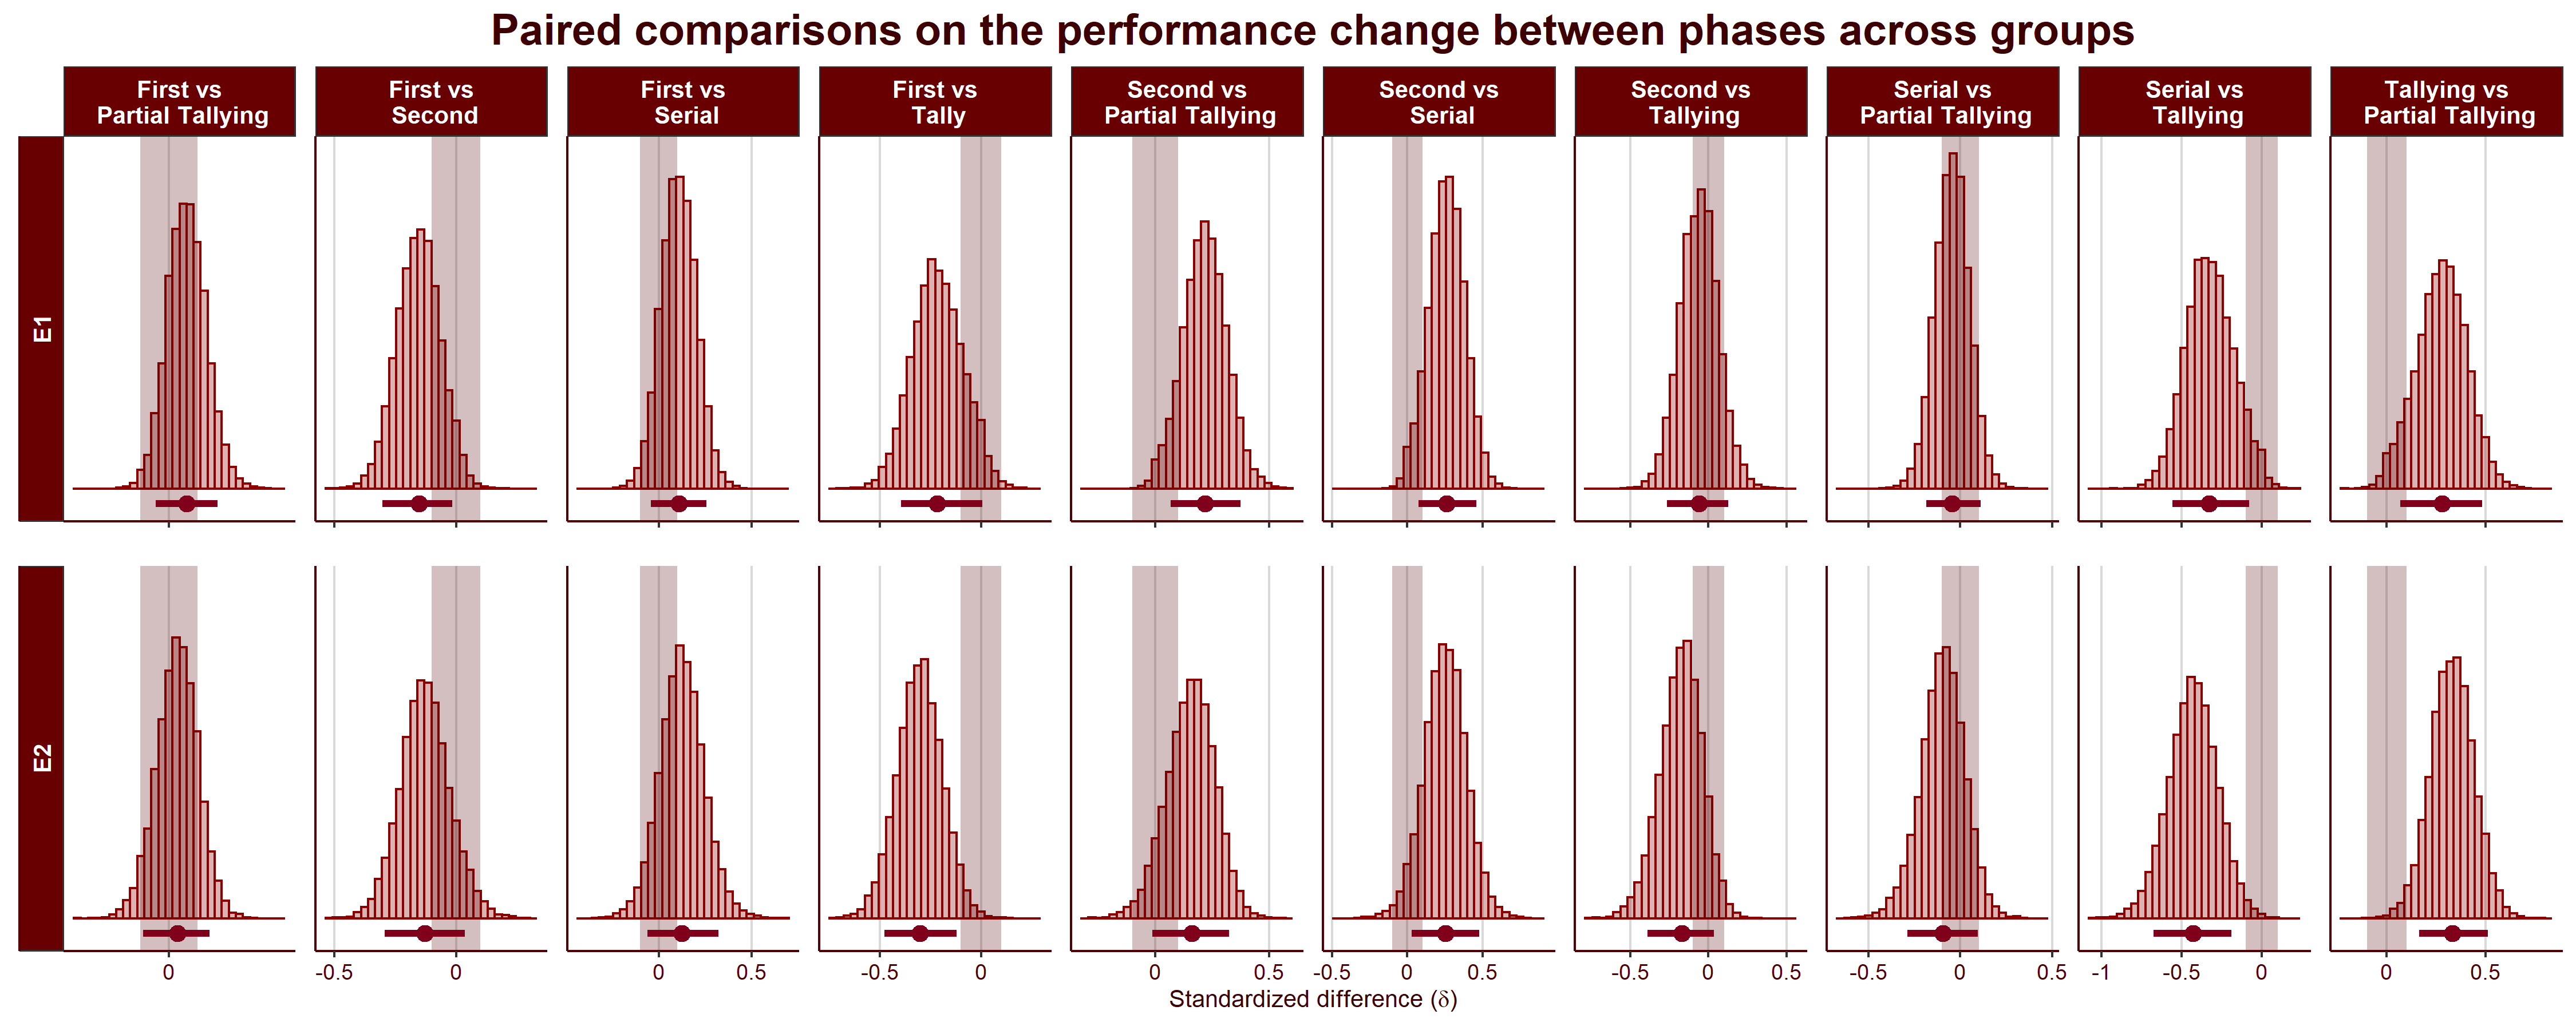
\includegraphics{C:/Users/rerr_/Google Drive/Graduate/Lab/Studies/MultiCue_Probabilistic/Stages/Shifted Weights/Eye Tracking/Analysis/Figures/SB2_performance_change_group.png}
\caption{\label{fig:performance-change-group}Paired comparisons between
groupds on their performance change across phases. The horizontal red
bar represents the 0.89 HDI. The shaded area highlights the ROPE used in
these comparisons}
\end{figure}

\begin{figure}
\centering
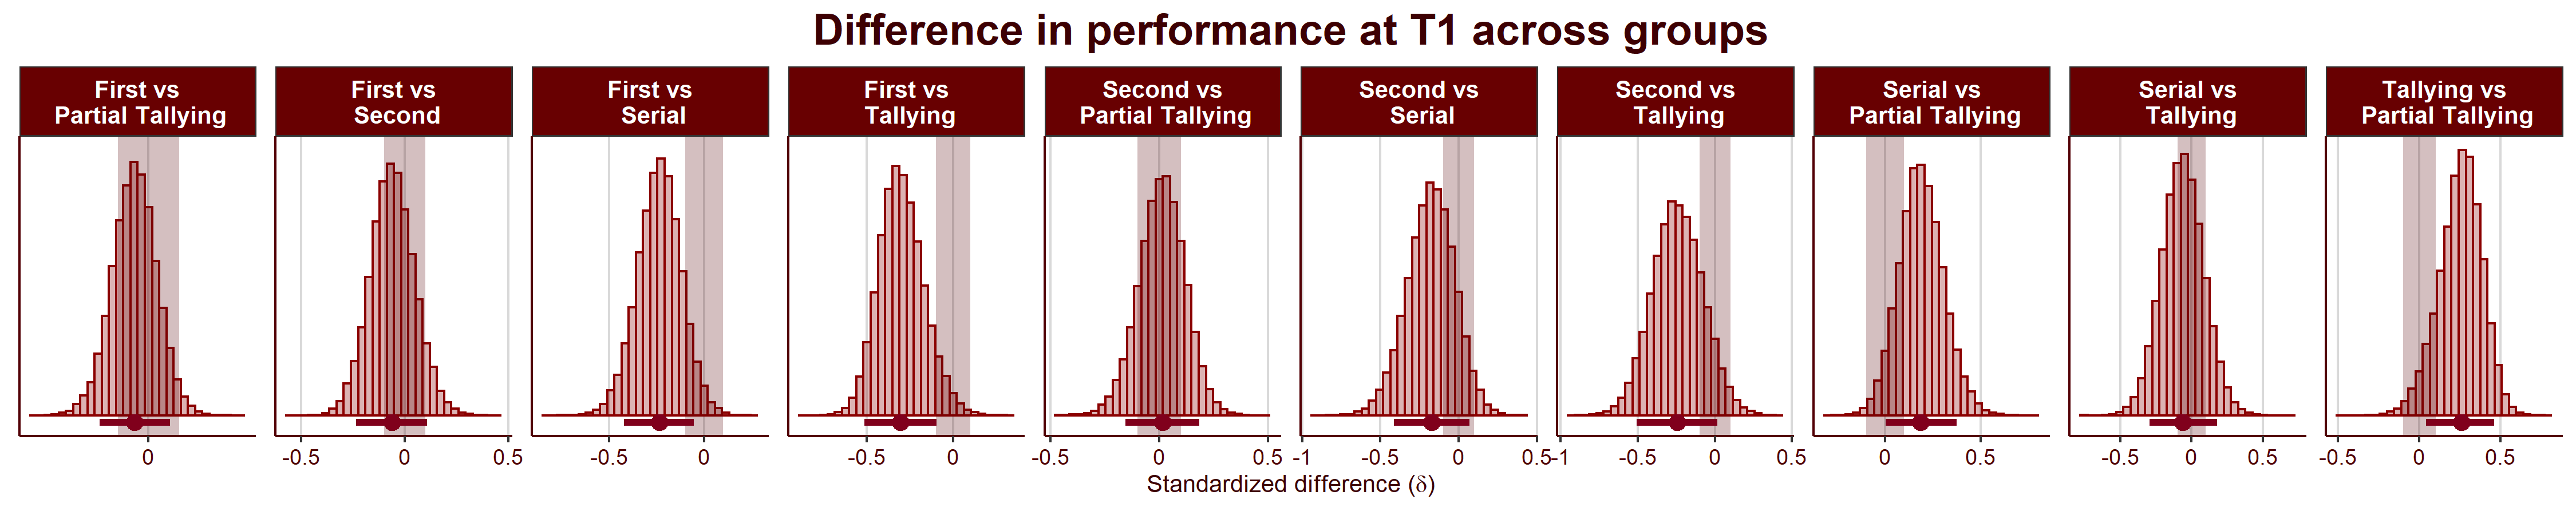
\includegraphics{C:/Users/rerr_/Google Drive/Graduate/Lab/Studies/MultiCue_Probabilistic/Stages/Shifted Weights/Eye Tracking/Analysis/Figures/SB3_performance_T1.png}
\caption{\label{fig:performance-T1}Difference in performance (as
standardized difference) at T1 across decision groups. The horizontal
red bar represents the 0.89 HDI. The shaded area highlights the ROPE
used in these comparisons}
\end{figure}

\begin{figure}
\centering
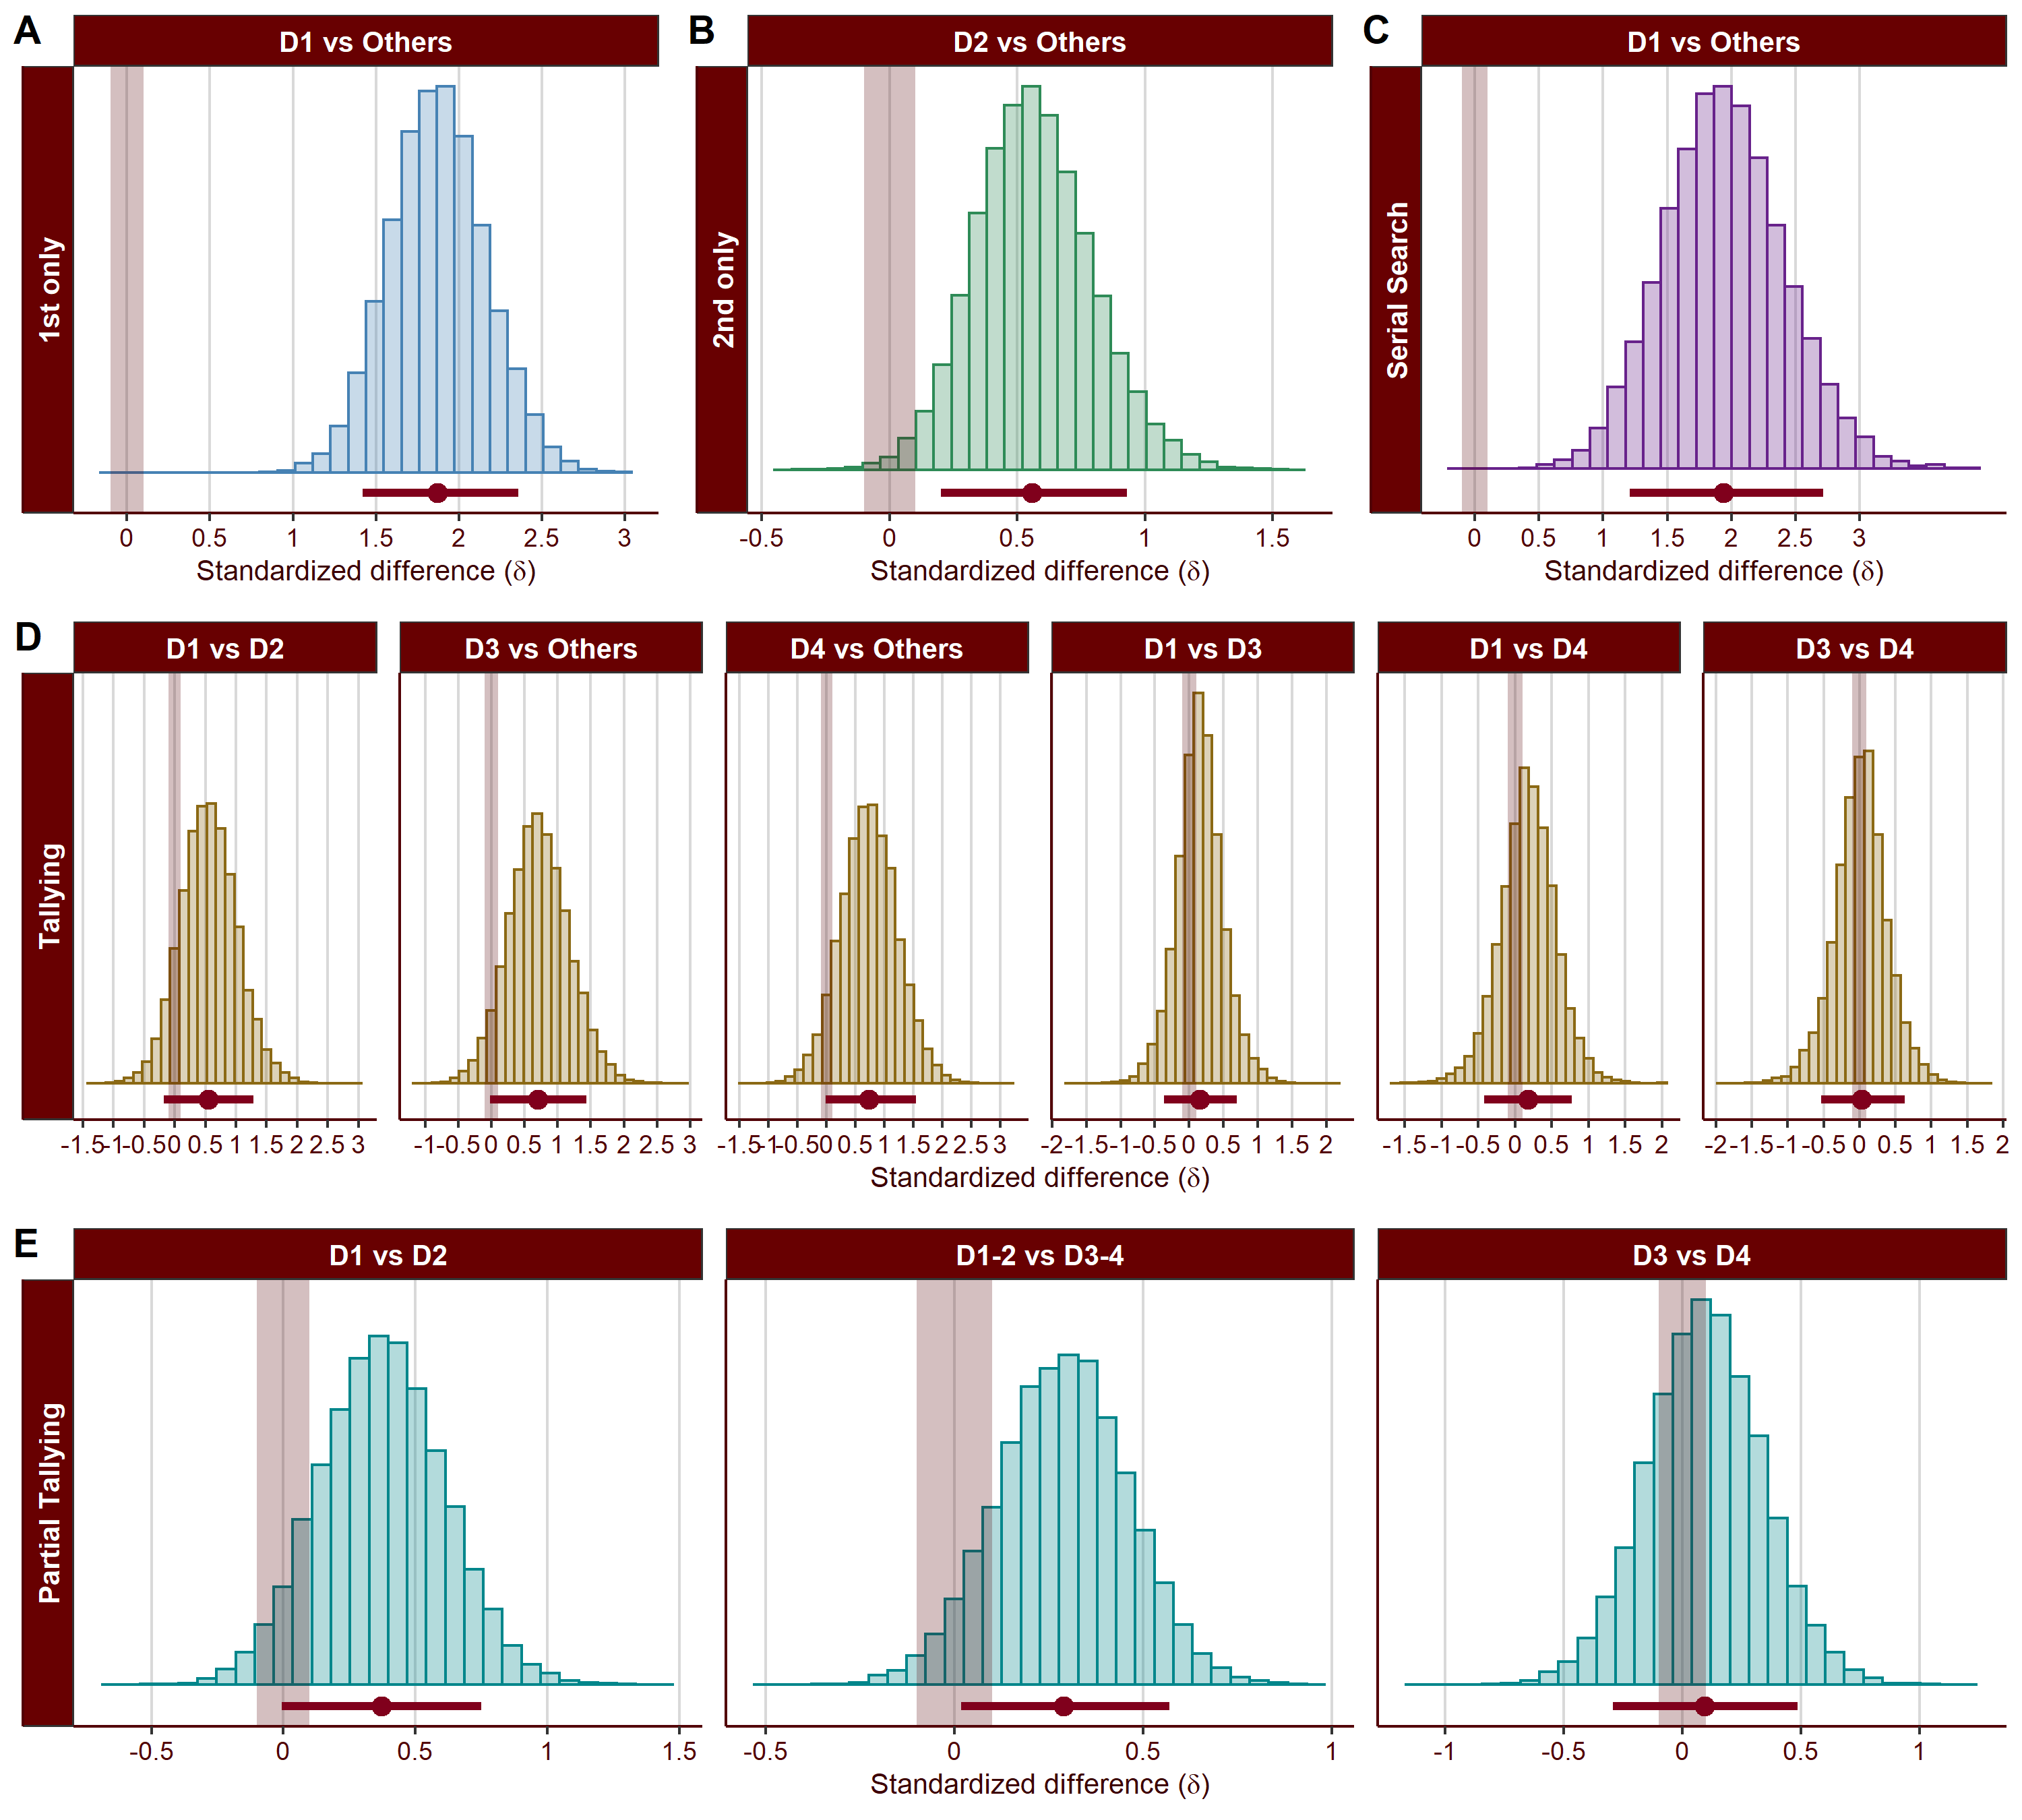
\includegraphics{C:/Users/rerr_/Google Drive/Graduate/Lab/Studies/MultiCue_Probabilistic/Stages/Shifted Weights/Eye Tracking/Analysis/Figures/SC1_first_comparisons.png}
\caption{\label{fig:first-comparisons}Follow up comparisons for the
allocation of first fixations, across decision groups. The horizontal
red bar represents the 0.89 HDI. The shaded area highlights the ROPE
used in these comparisons}
\end{figure}

\begin{figure}
\centering
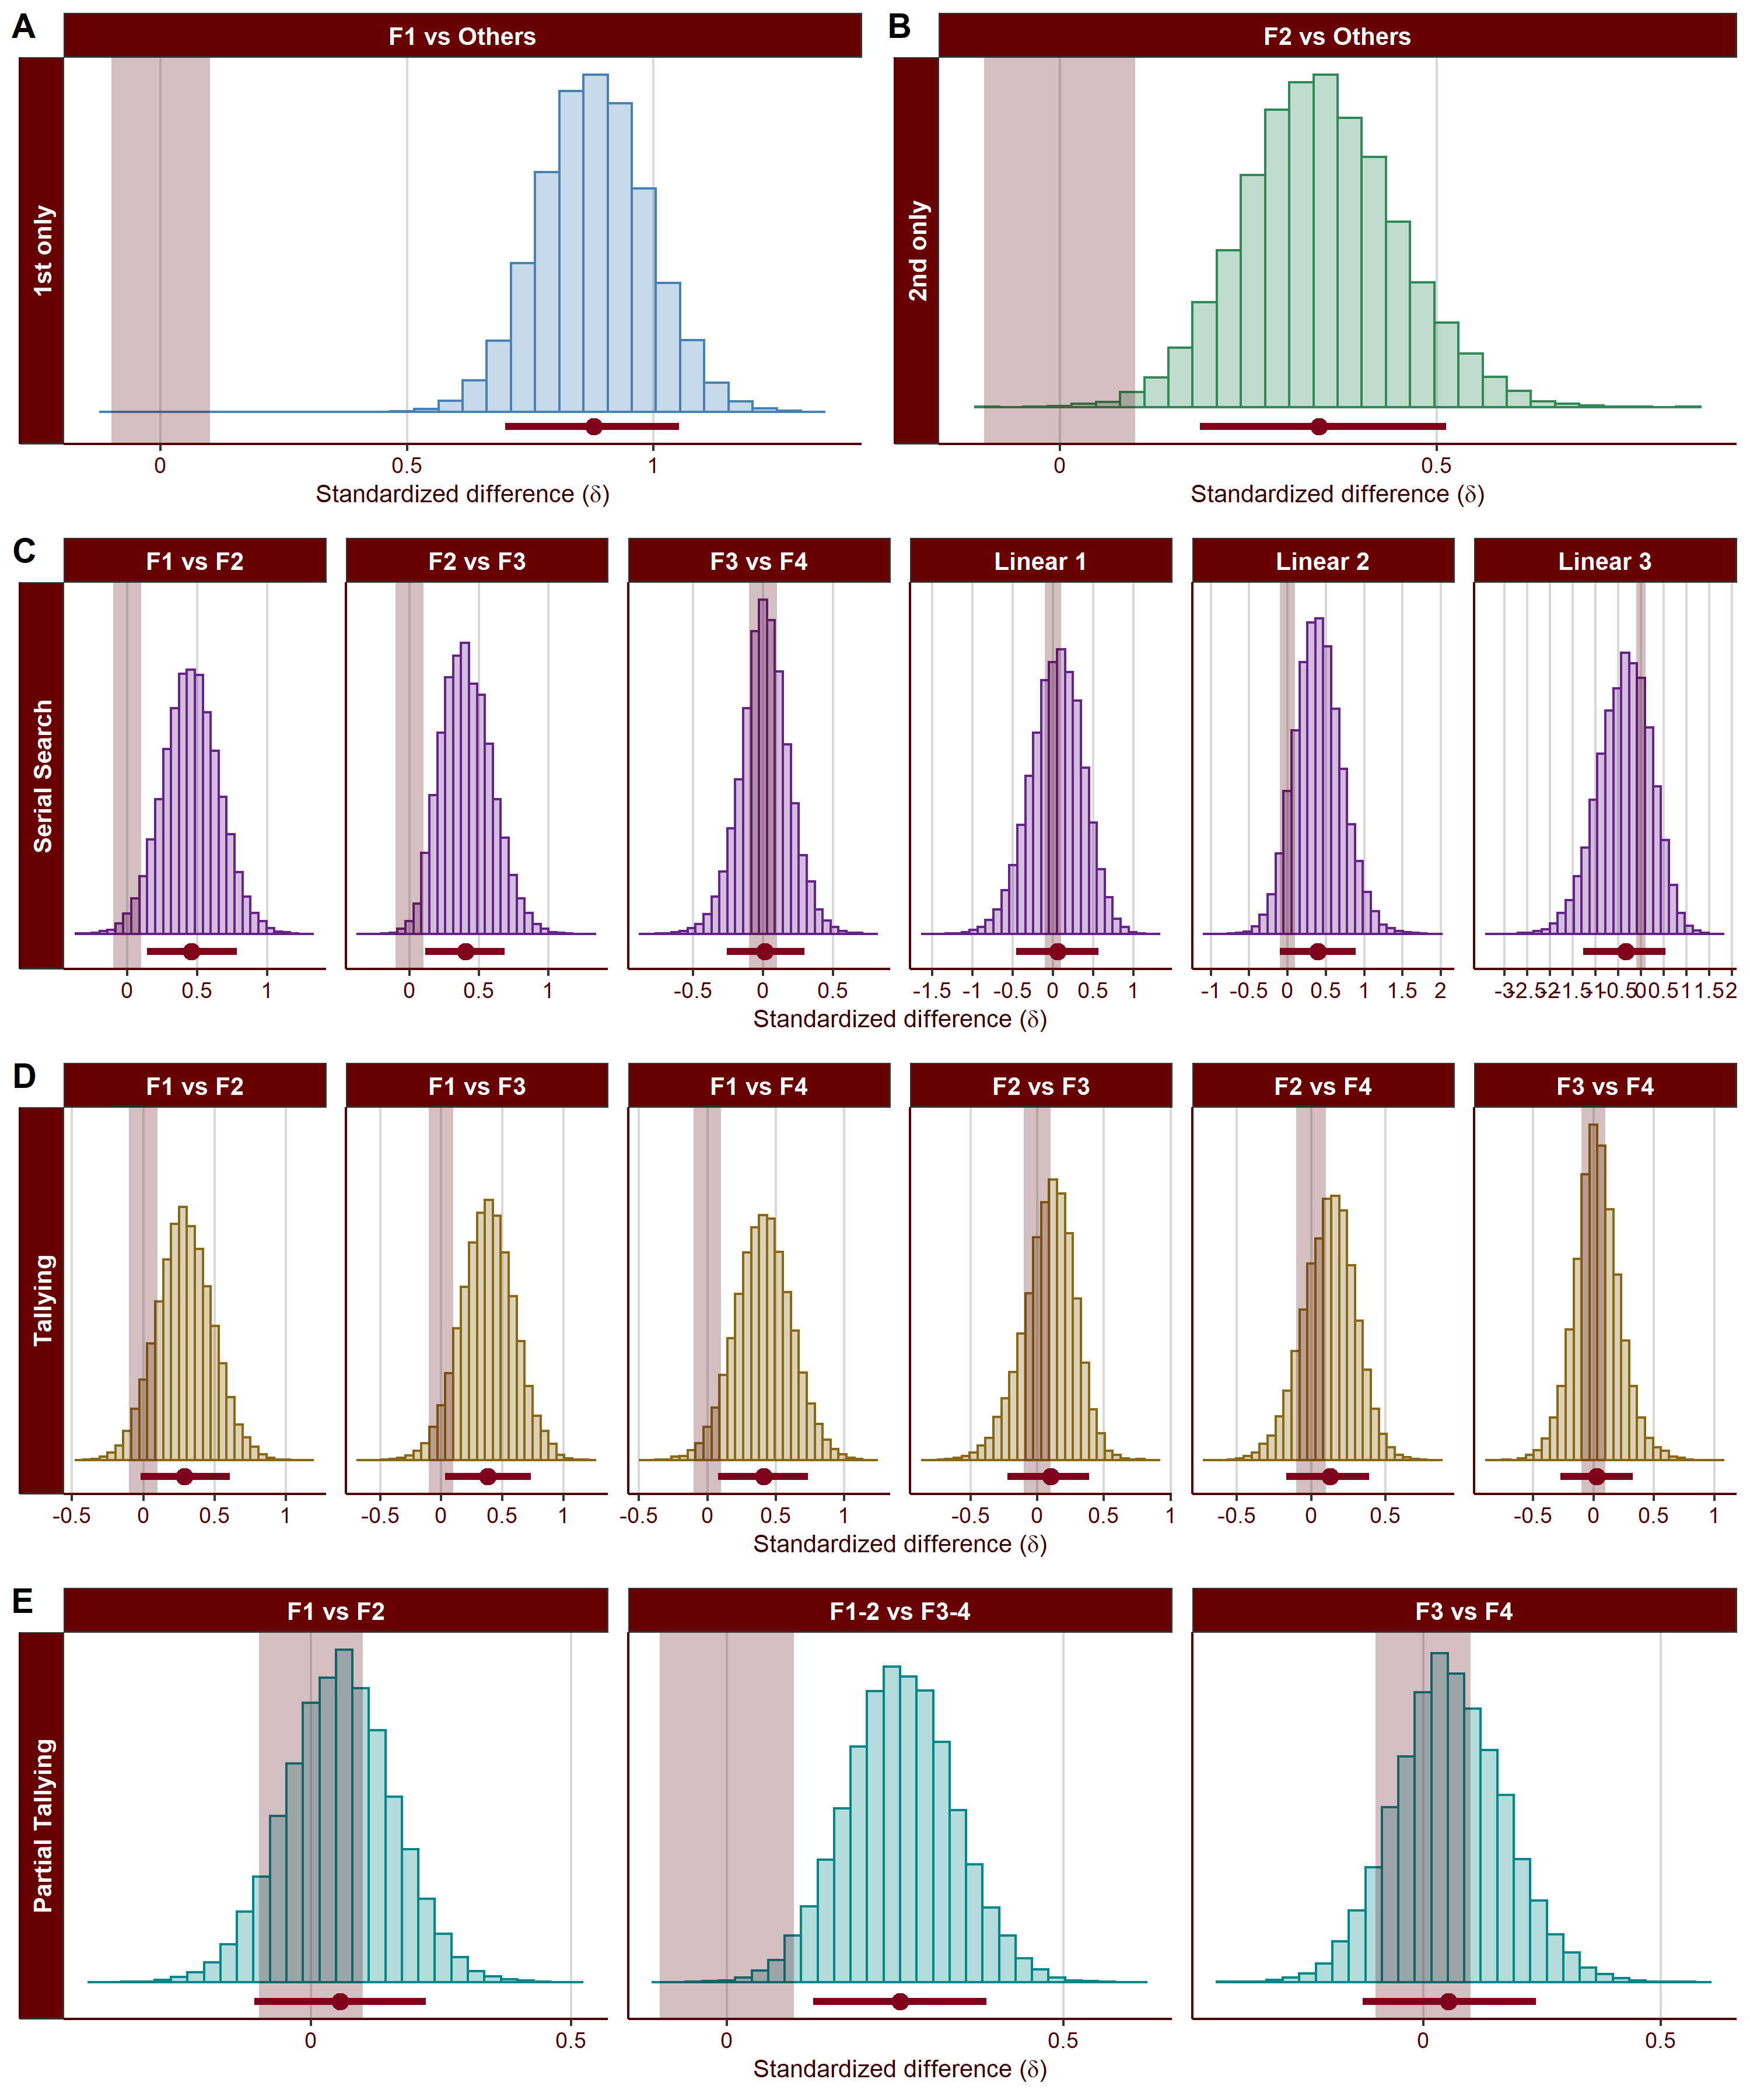
\includegraphics{C:/Users/rerr_/Google Drive/Graduate/Lab/Studies/MultiCue_Probabilistic/Stages/Shifted Weights/Eye Tracking/Analysis/Figures/SD1_proportion_comparisons.png}
\caption{\label{fig:proportion-comparisons}Follow up comparisons for the
allocation of fixations. The horizontal red bar represents the 0.89 HDI.
The shaded area highlights the ROPE used in these comparisons}
\end{figure}

\begin{figure}
\centering
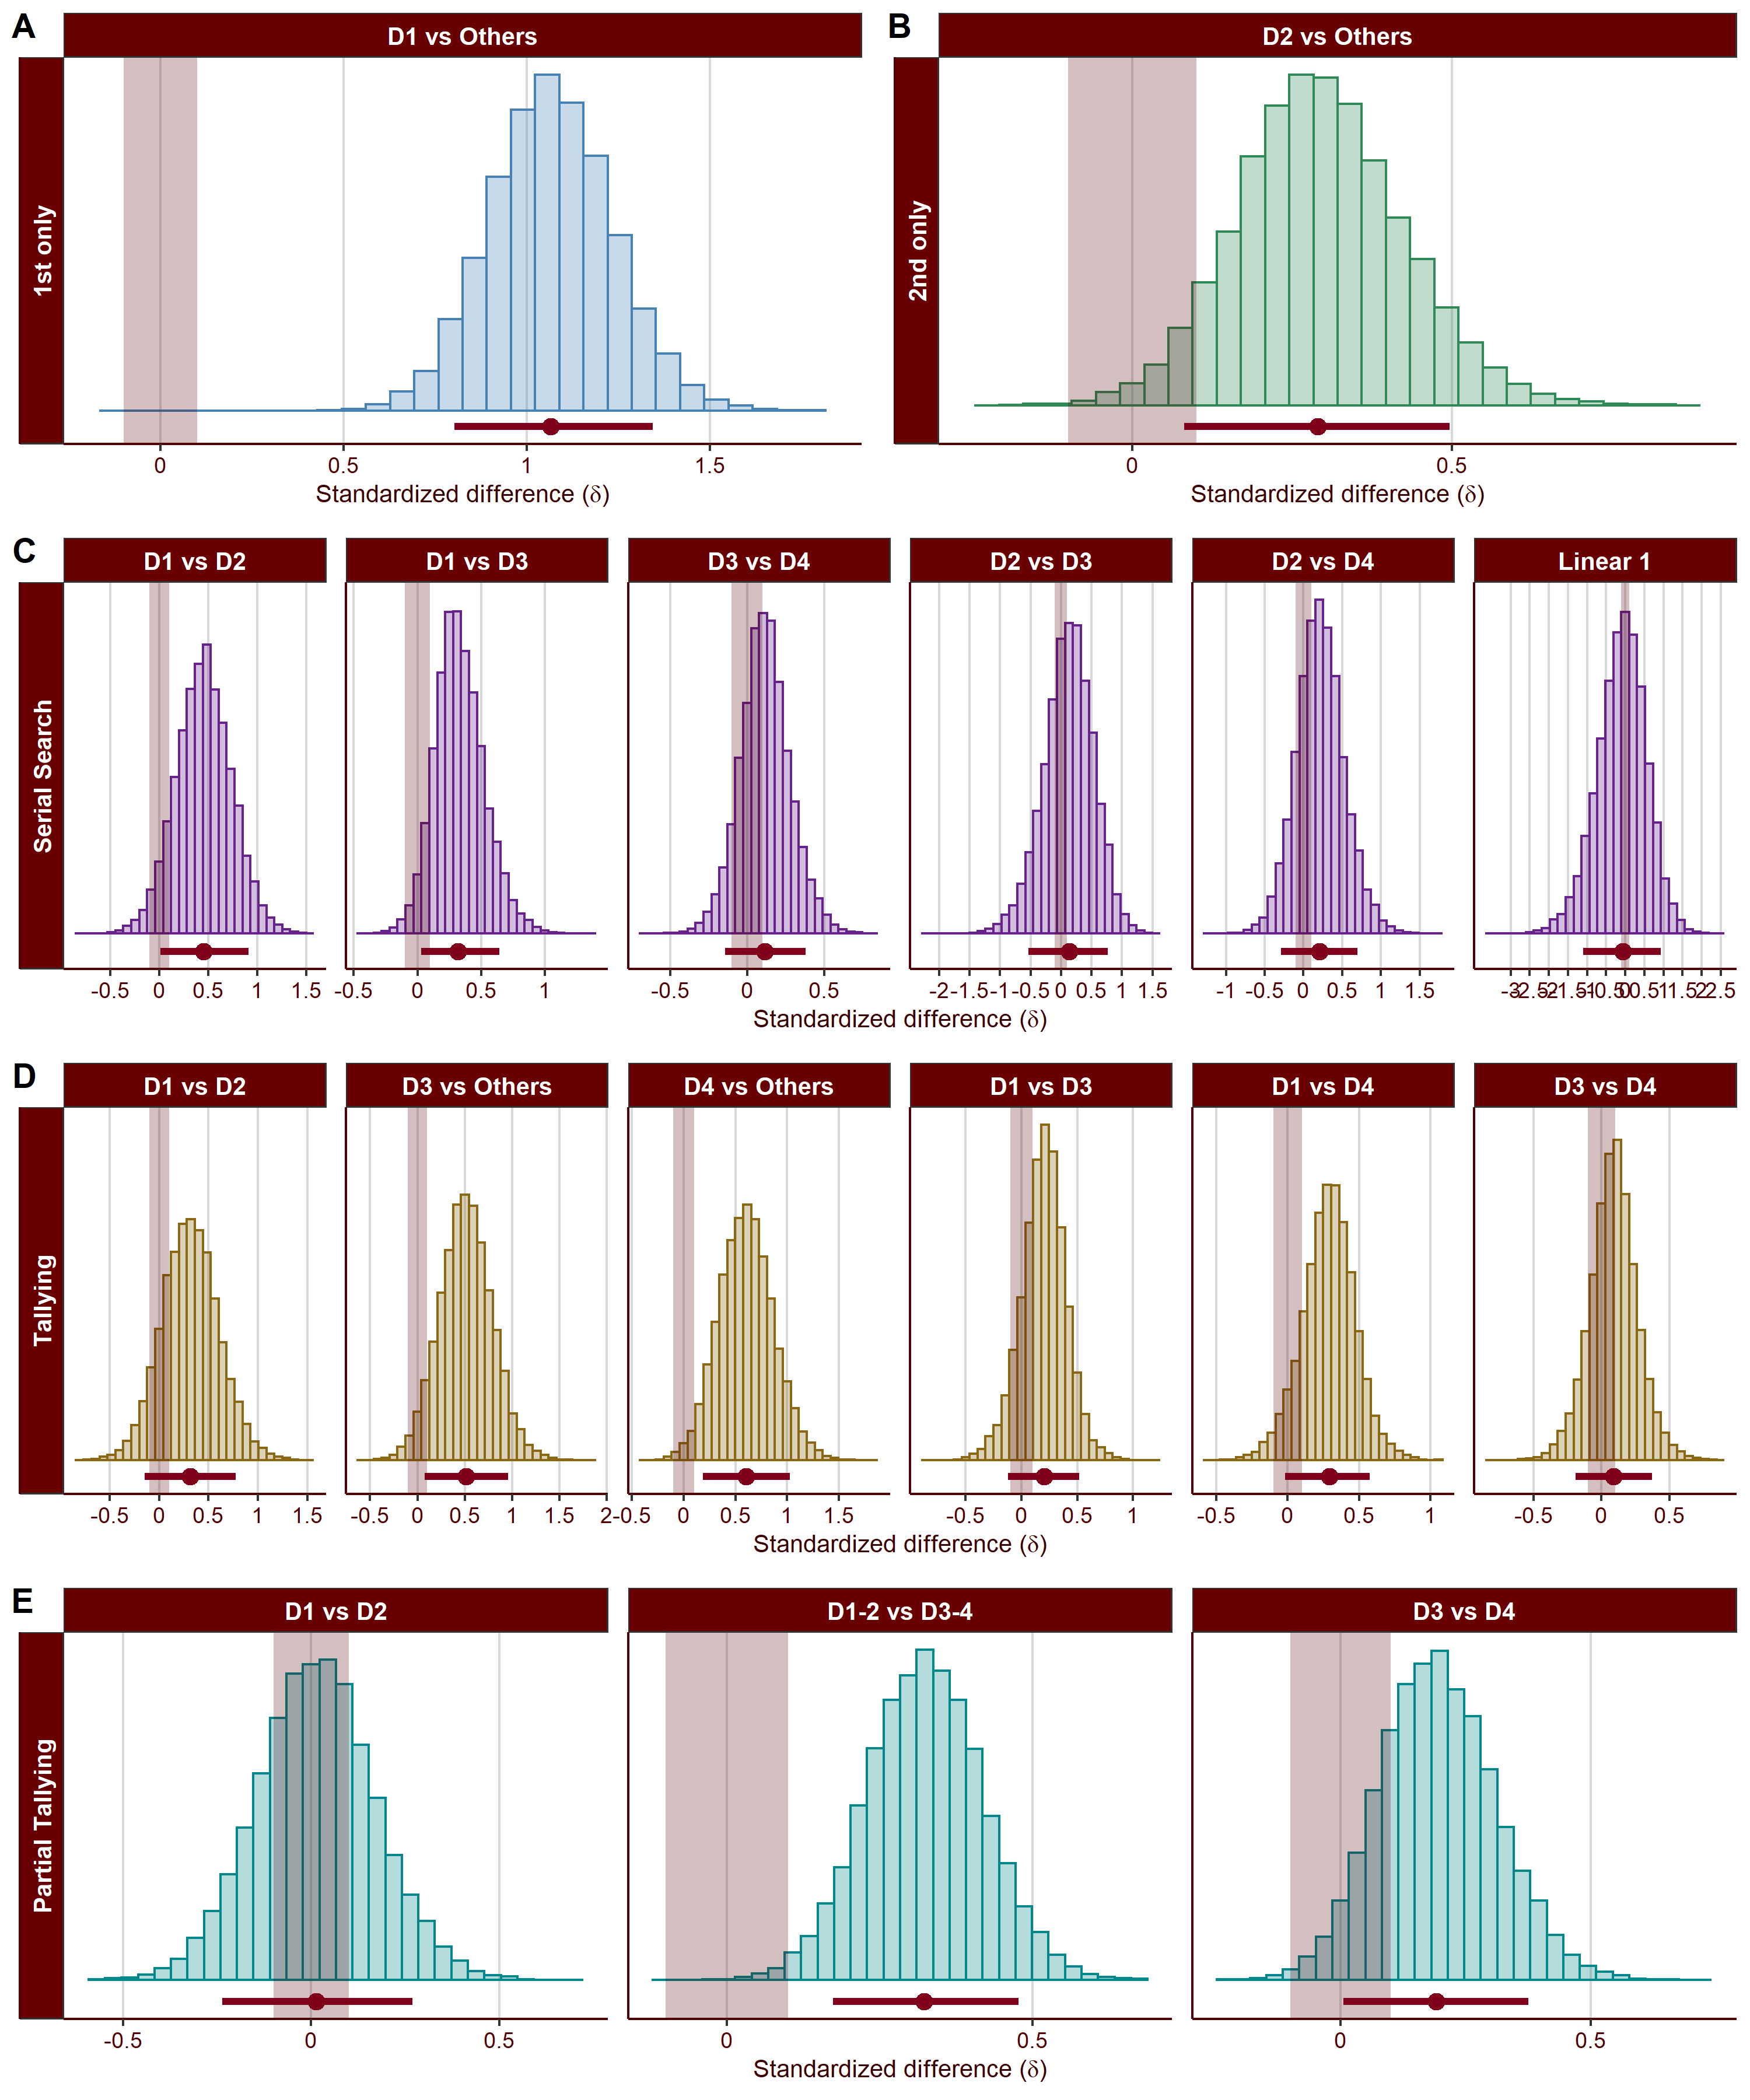
\includegraphics{C:/Users/rerr_/Google Drive/Graduate/Lab/Studies/MultiCue_Probabilistic/Stages/Shifted Weights/Eye Tracking/Analysis/Figures/SE1_last_comparisons.png}
\caption{\label{fig:last-comparisons}Follow up comparisons for the
allocation of last fixations. The horizontal red bar represents the 0.89
HDI. The shaded area highlights the ROPE used in these comparisons}
\end{figure}

\begin{figure}[!b]
\centering
\begin{subfigure}{1\textwidth}
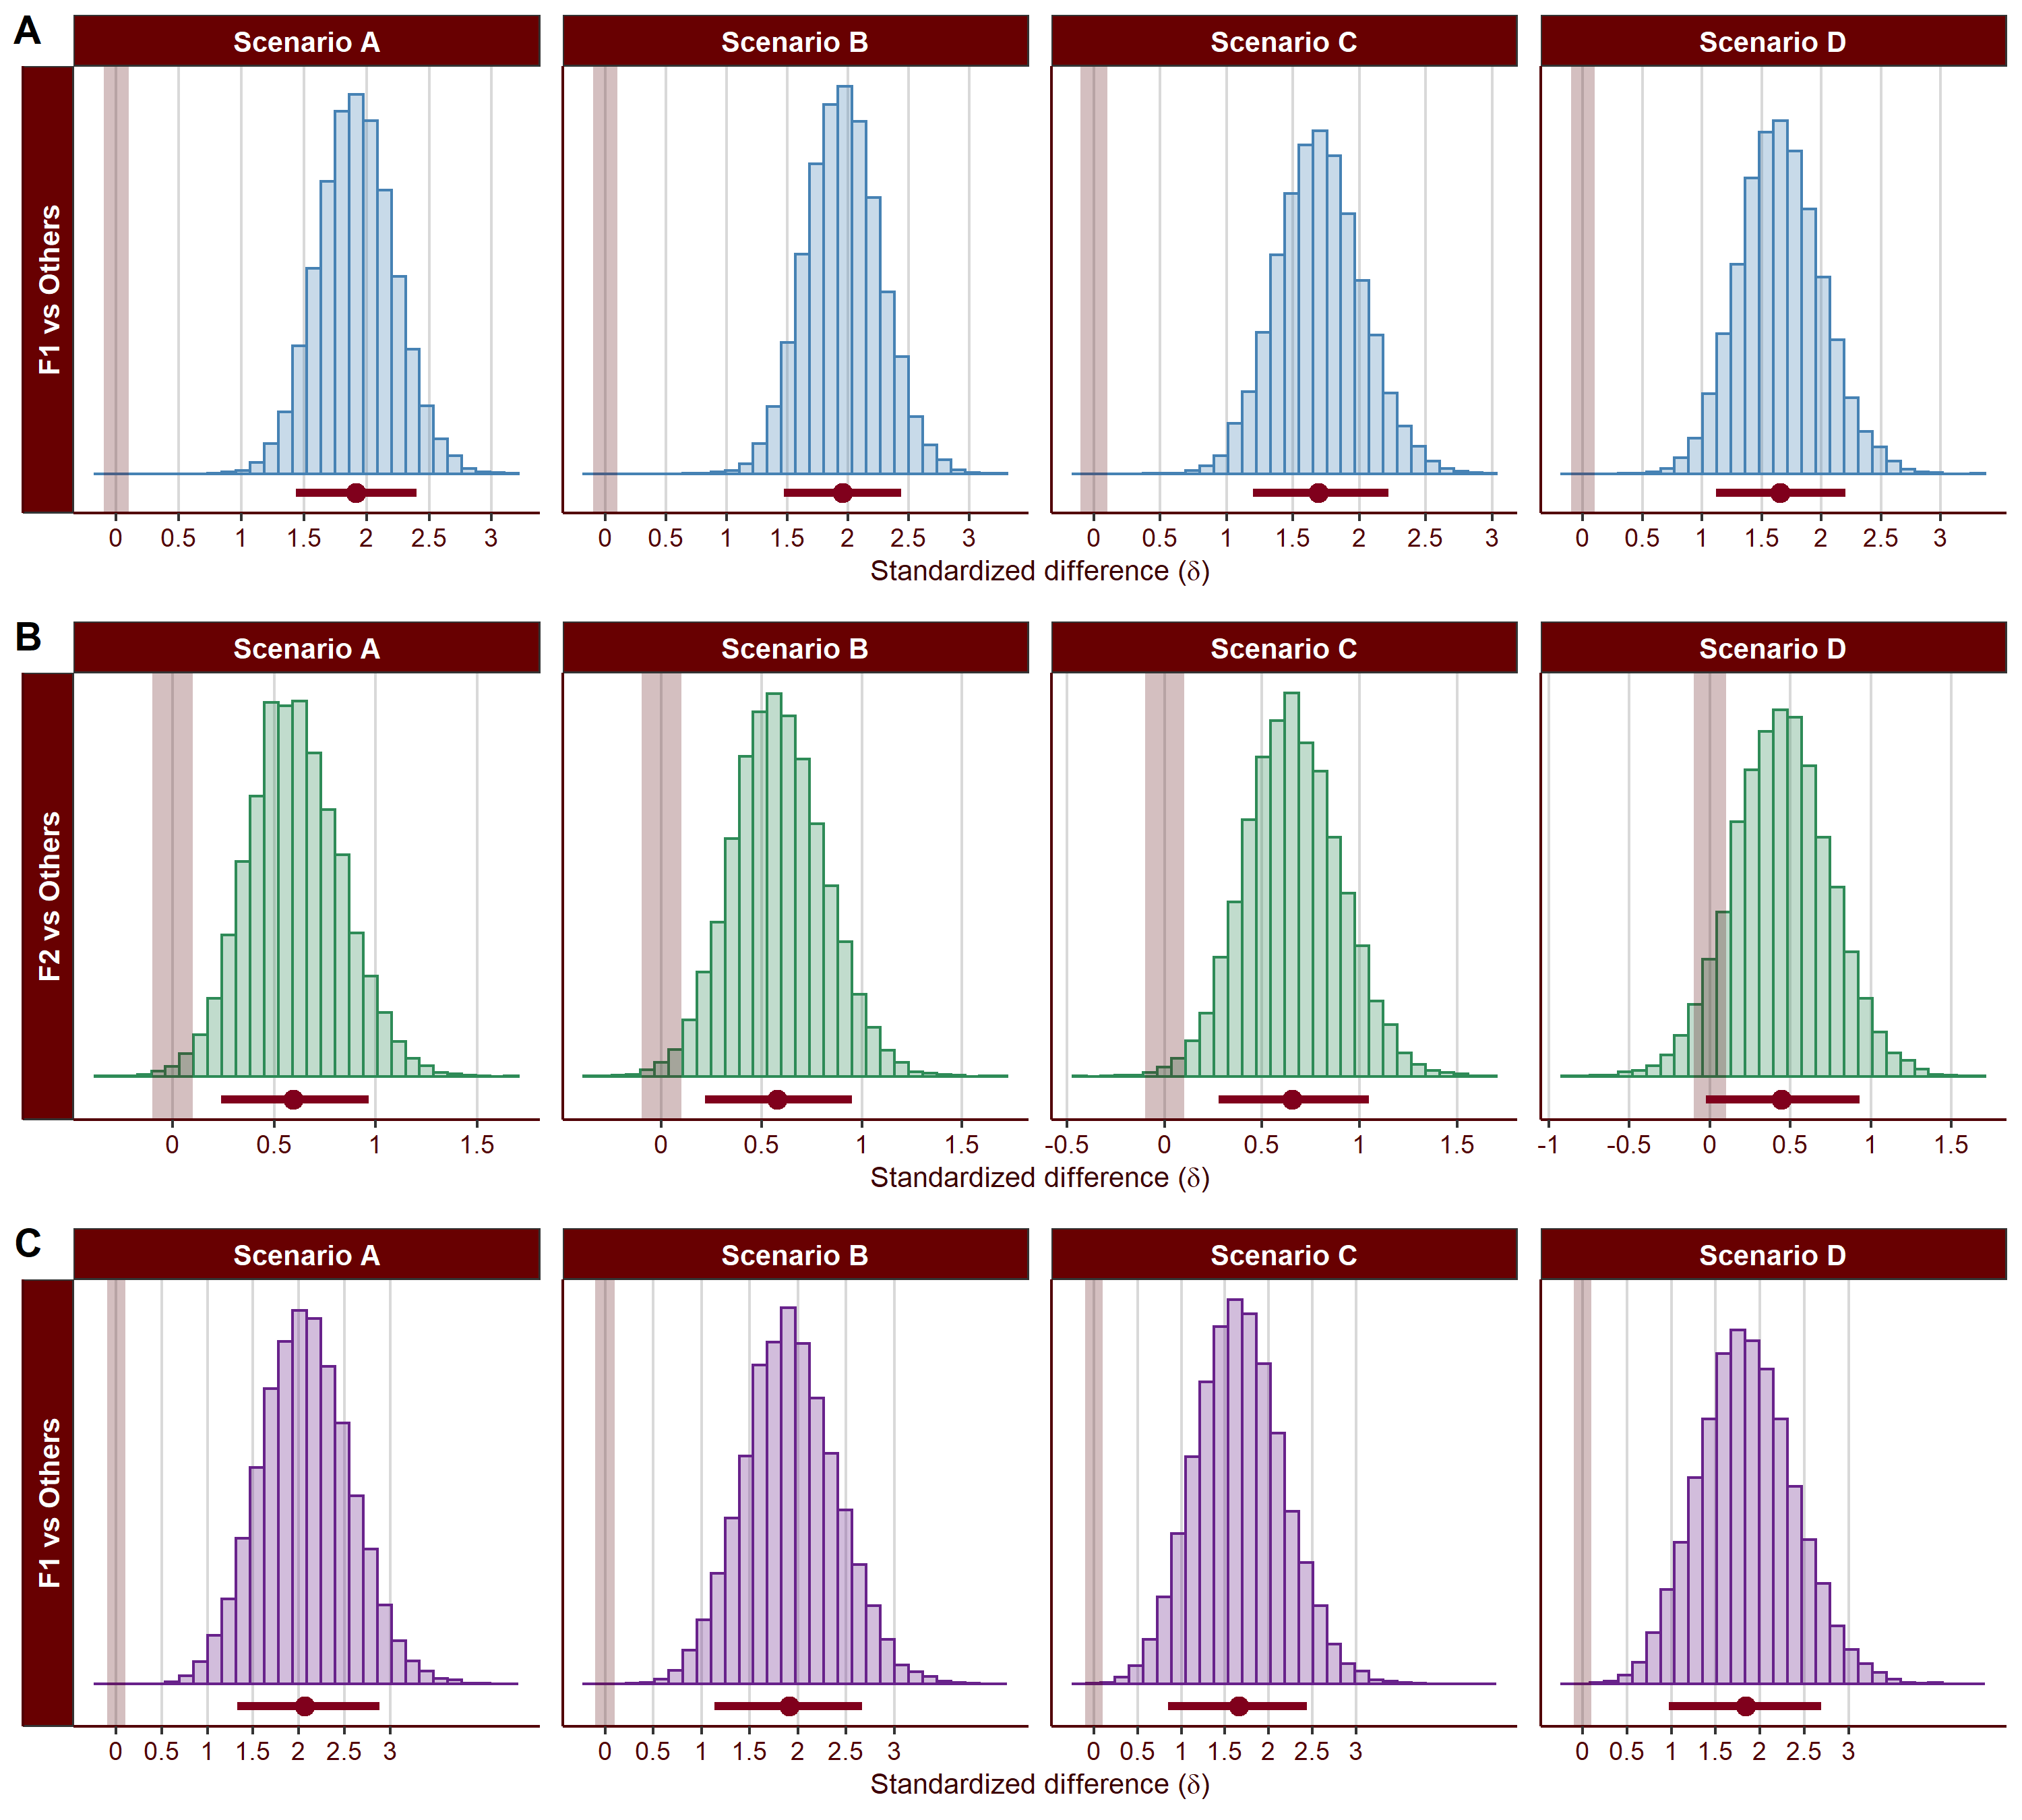
\includegraphics[width=\linewidth]{Figures/SC2_first_scenario_comparisons_A.png}
\subcaption{1st only (A), 2nd only (B), Serial search (C)}
\label{fig:first-scenario-comparisons-A}
\end{subfigure}
\caption[]{Follow up comparisons for the allocation of first fixations across decision groups in the different decision scenarios. The horizontal red bar represents the 0.89 HDI. The shaded area highlights the ROPE used in these comparisons}
\end{figure}

\medskip

\begin{figure}[ht]\ContinuedFloat
\centering
\begin{subfigure}{1\textwidth}
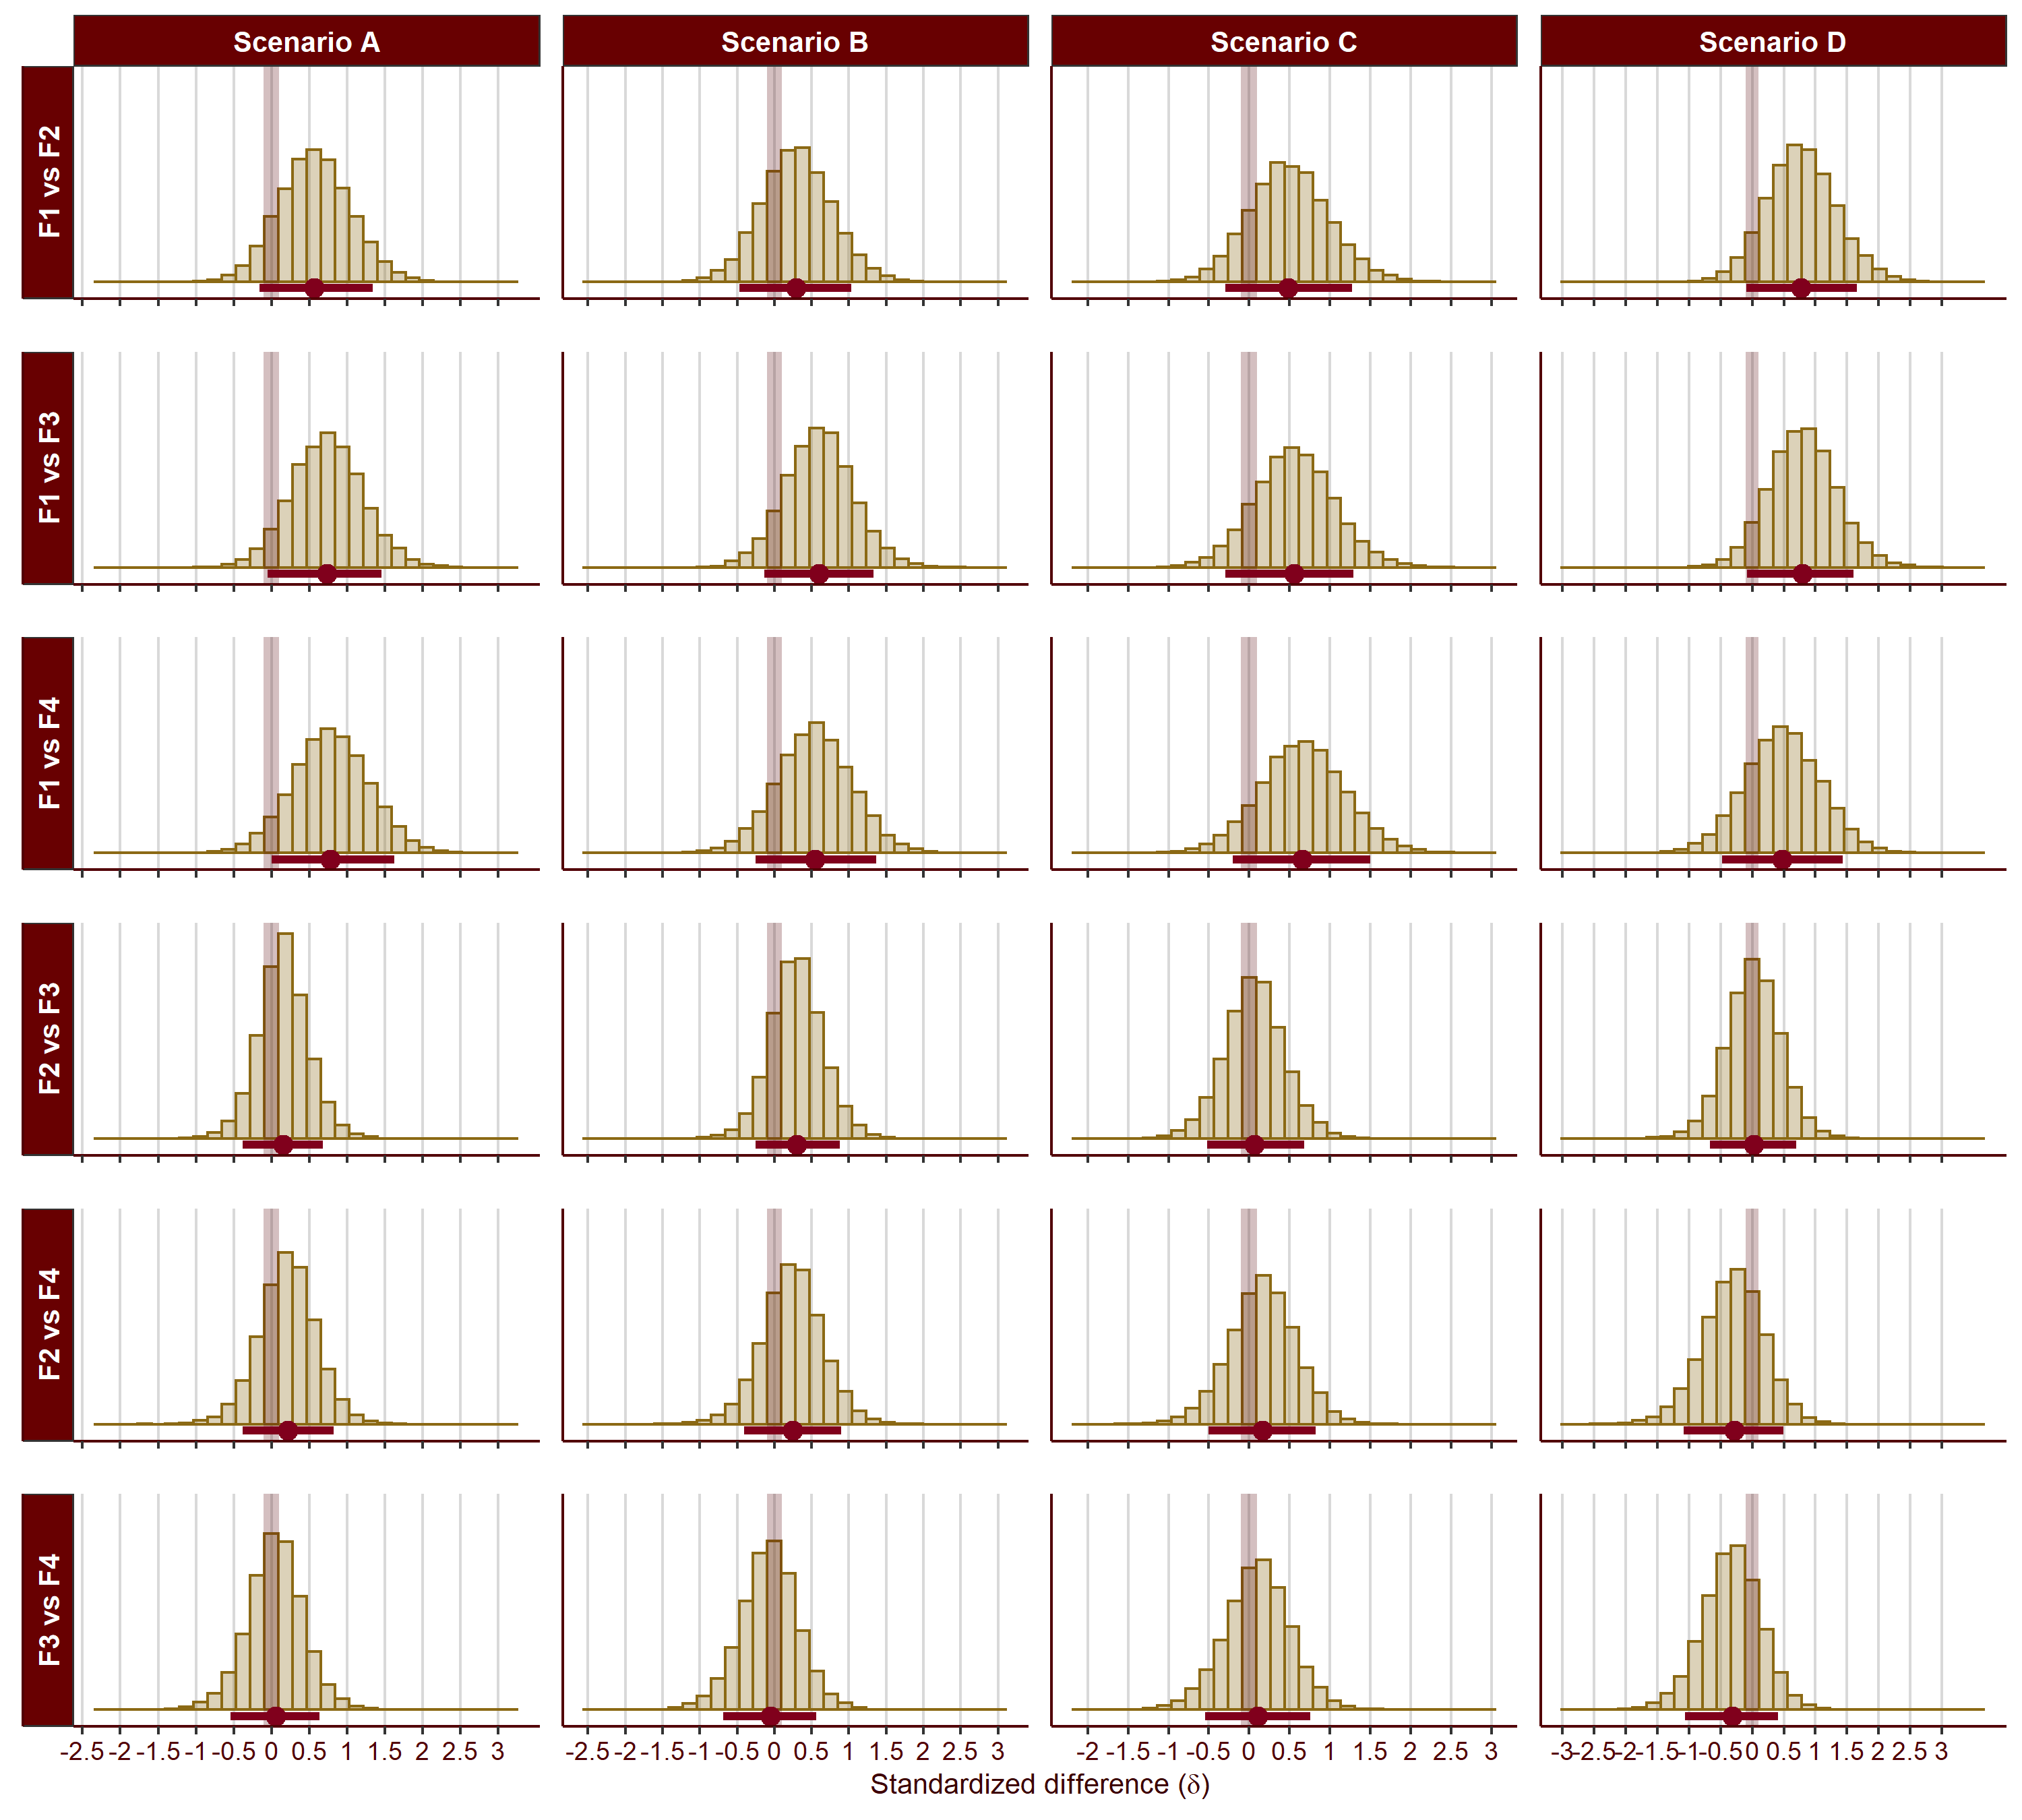
\includegraphics[width=\linewidth]{Figures/SC2_first_scenario_comparisons_B.png}
\subcaption{Tallying}
\label{fig:first-scenario-comparisons-B}
\end{subfigure}
\caption[]{Continued}
\end{figure}

\medskip

\begin{figure}[ht]\ContinuedFloat
\centering
\begin{subfigure}{1\textwidth}
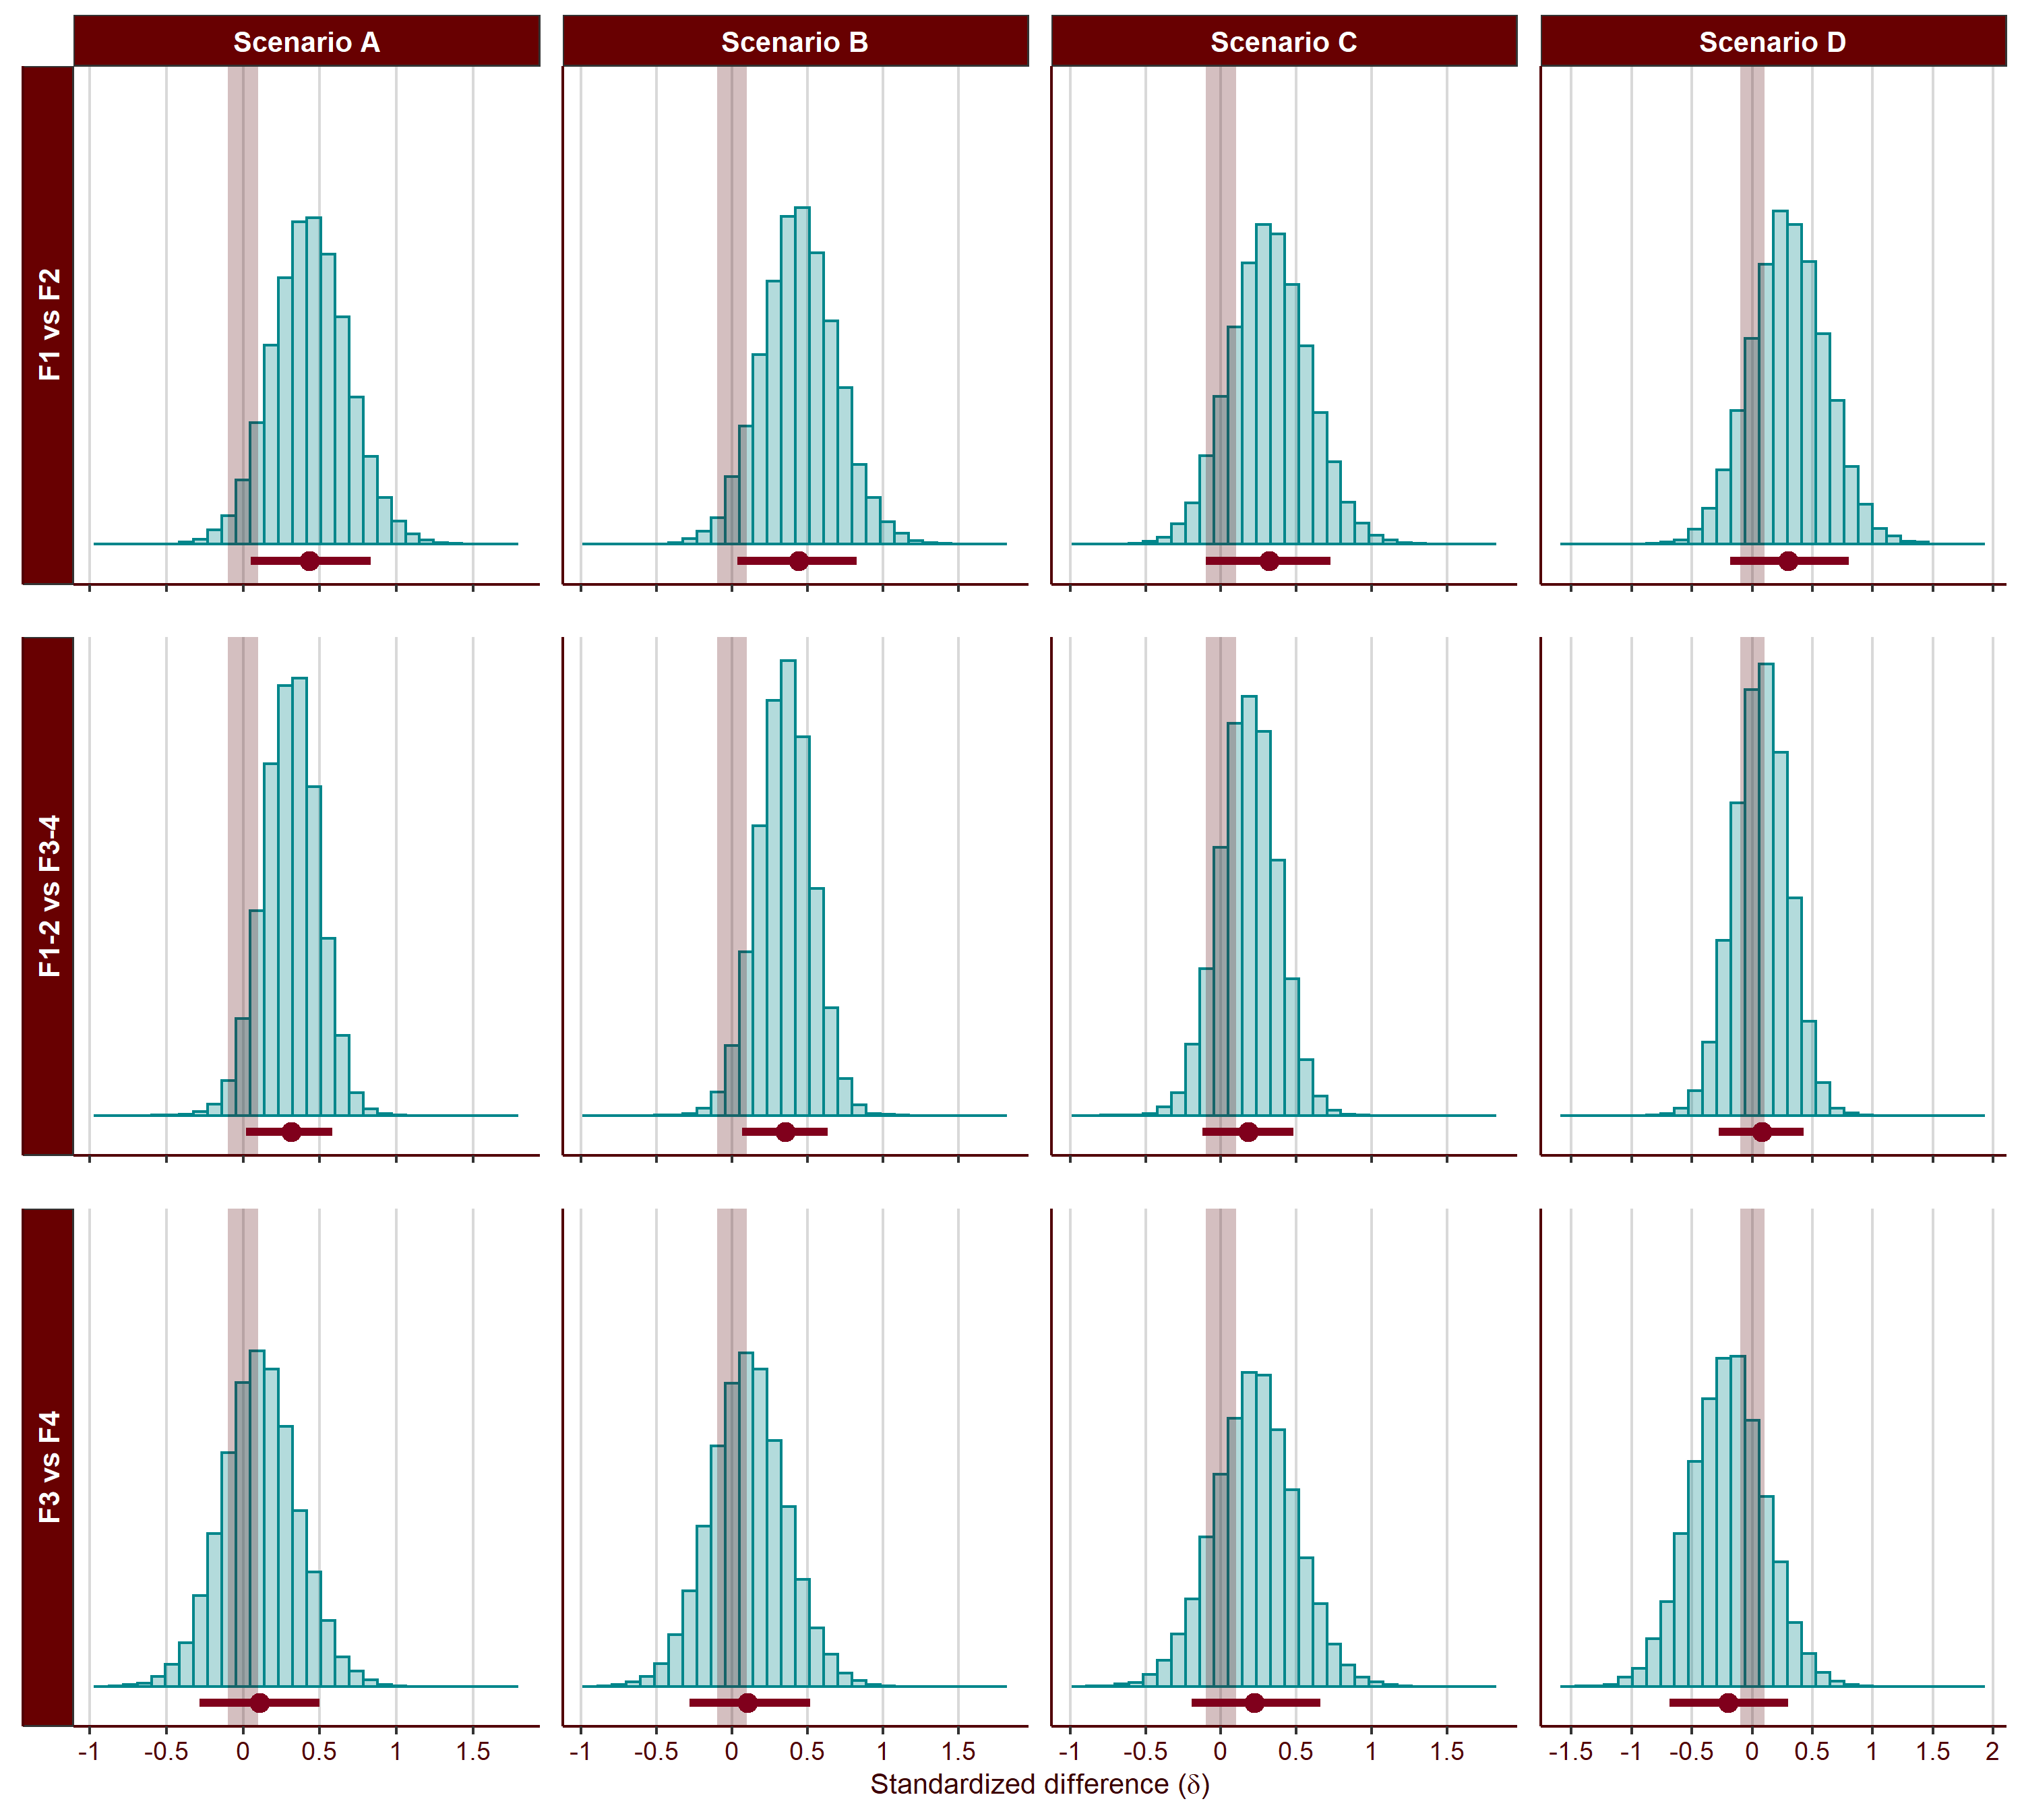
\includegraphics[width=\linewidth]{Figures/SC2_first_scenario_comparisons_C.png}
\subcaption{Partial Tallying}
\label{fig:first-scenario-comparisons-C}
\end{subfigure}
\caption[]{Continued}
\label{fig:first-scenario-comparisons}
\end{figure}

\begin{figure}[!b]
\centering
\begin{subfigure}{1\textwidth}
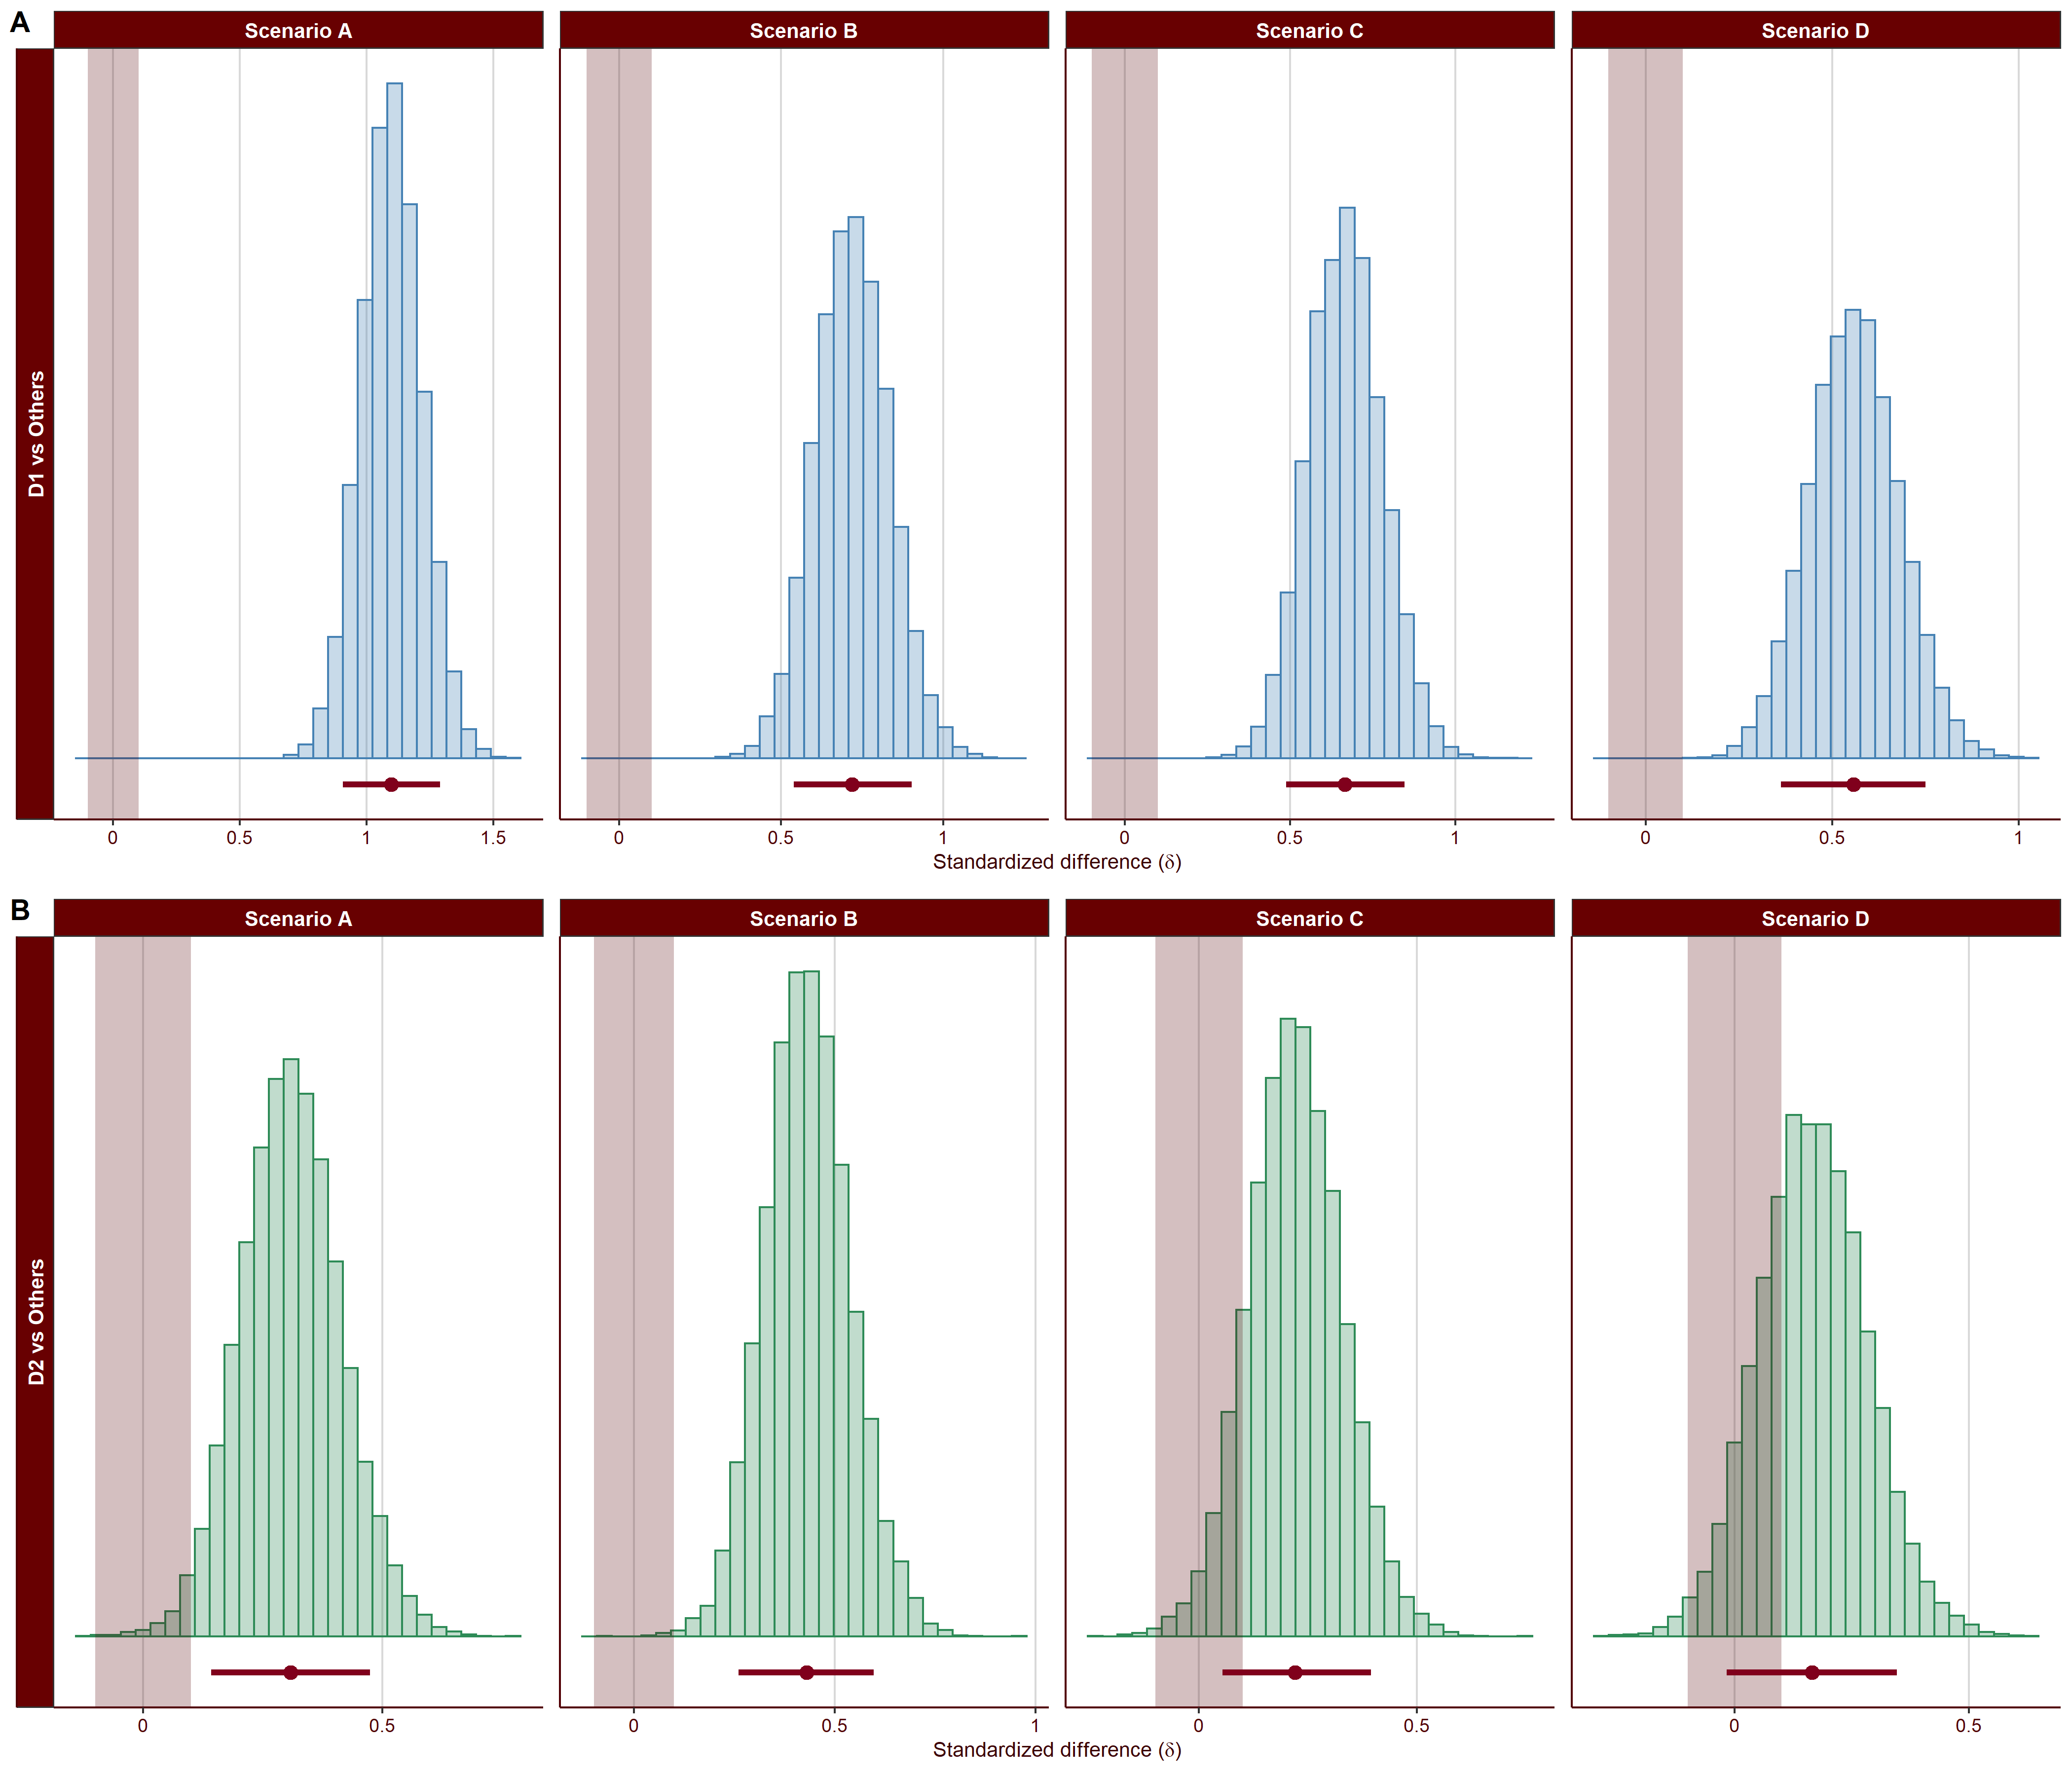
\includegraphics[width=\linewidth]{Figures/SD2_proportion_scenario_comparisons_A.png}
\subcaption{1st only (A), 2nd only (B)}
\label{fig:proportion-scenario-comparisons-A}
\end{subfigure}
\caption[]{Follow up comparisons for the allocation of fixations across decision groups in the different decision scenarios. The horizontal red bar represents the 0.89 HDI. The shaded area highlights the ROPE used in these comparisons}
\end{figure}

\medskip

\begin{figure}[ht]\ContinuedFloat
\centering
\begin{subfigure}{1\textwidth}
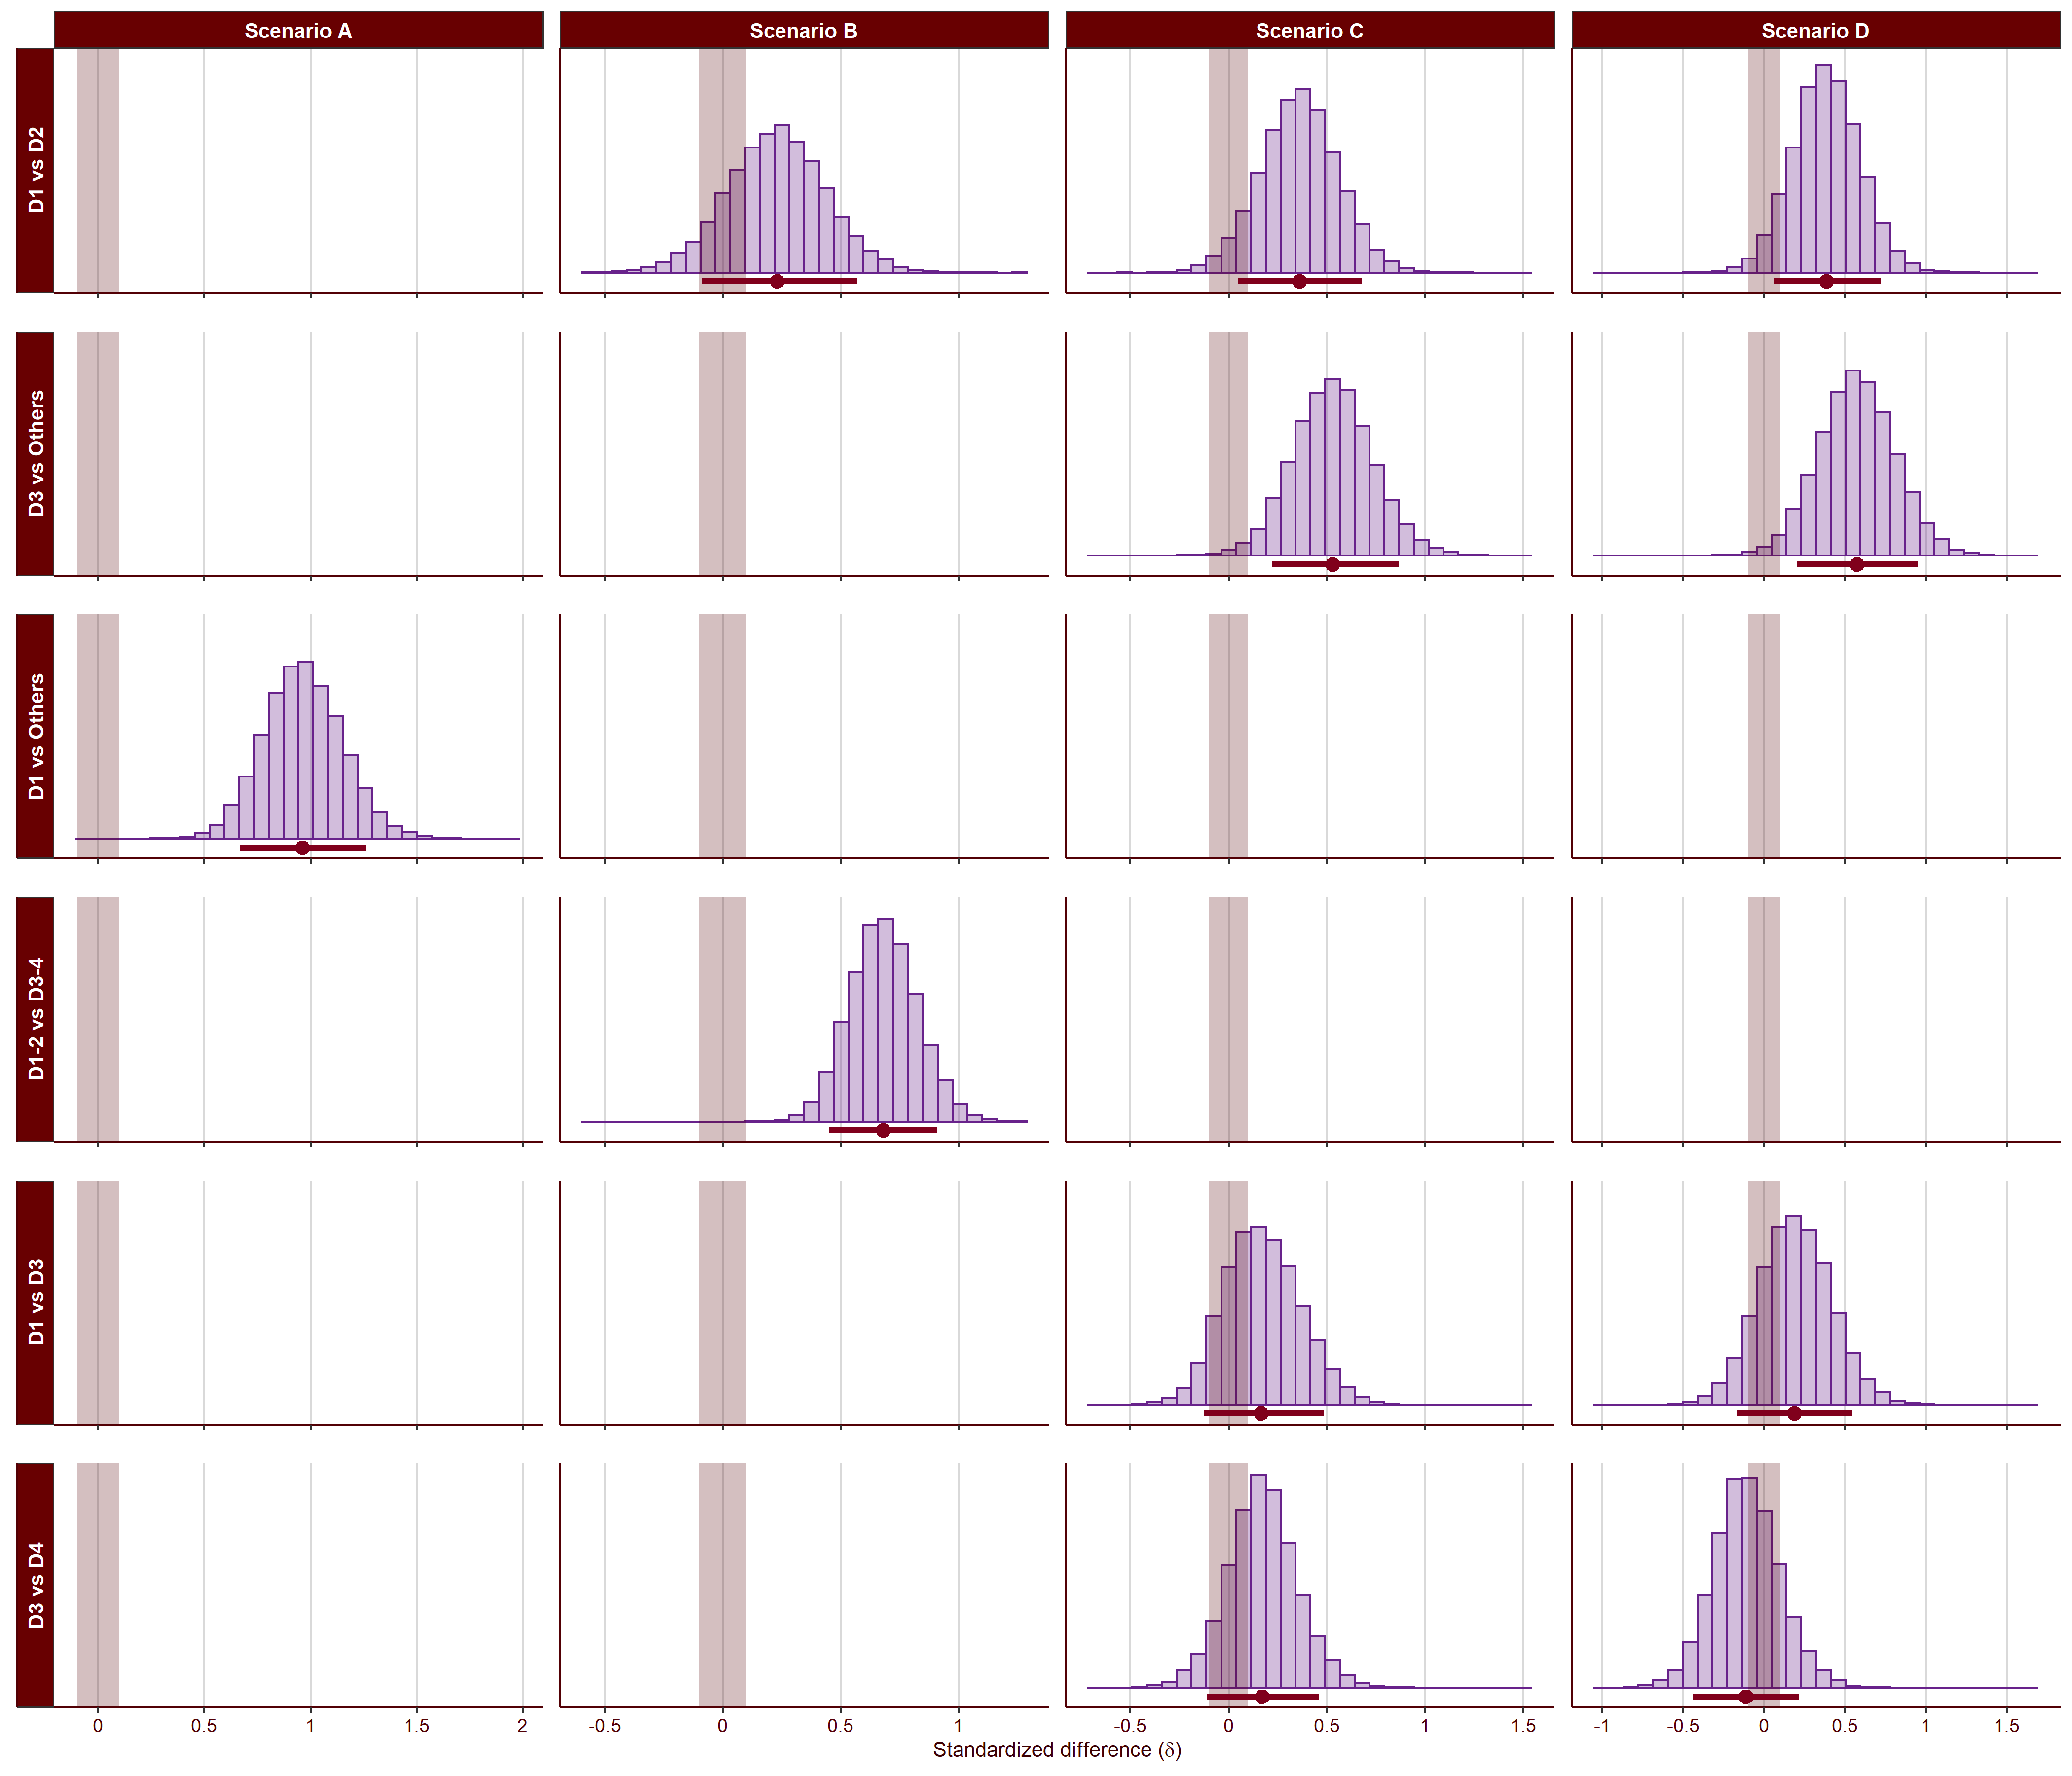
\includegraphics[width=\linewidth]{Figures/SD2_proportion_scenario_comparisons_B.png}
\subcaption{Serial Search}
\label{fig:proportion-scenario-comparisons-B}
\end{subfigure}
\caption[]{Continued}
\end{figure}

\medskip

\begin{figure}[ht]\ContinuedFloat
\centering
\begin{subfigure}{1\textwidth}
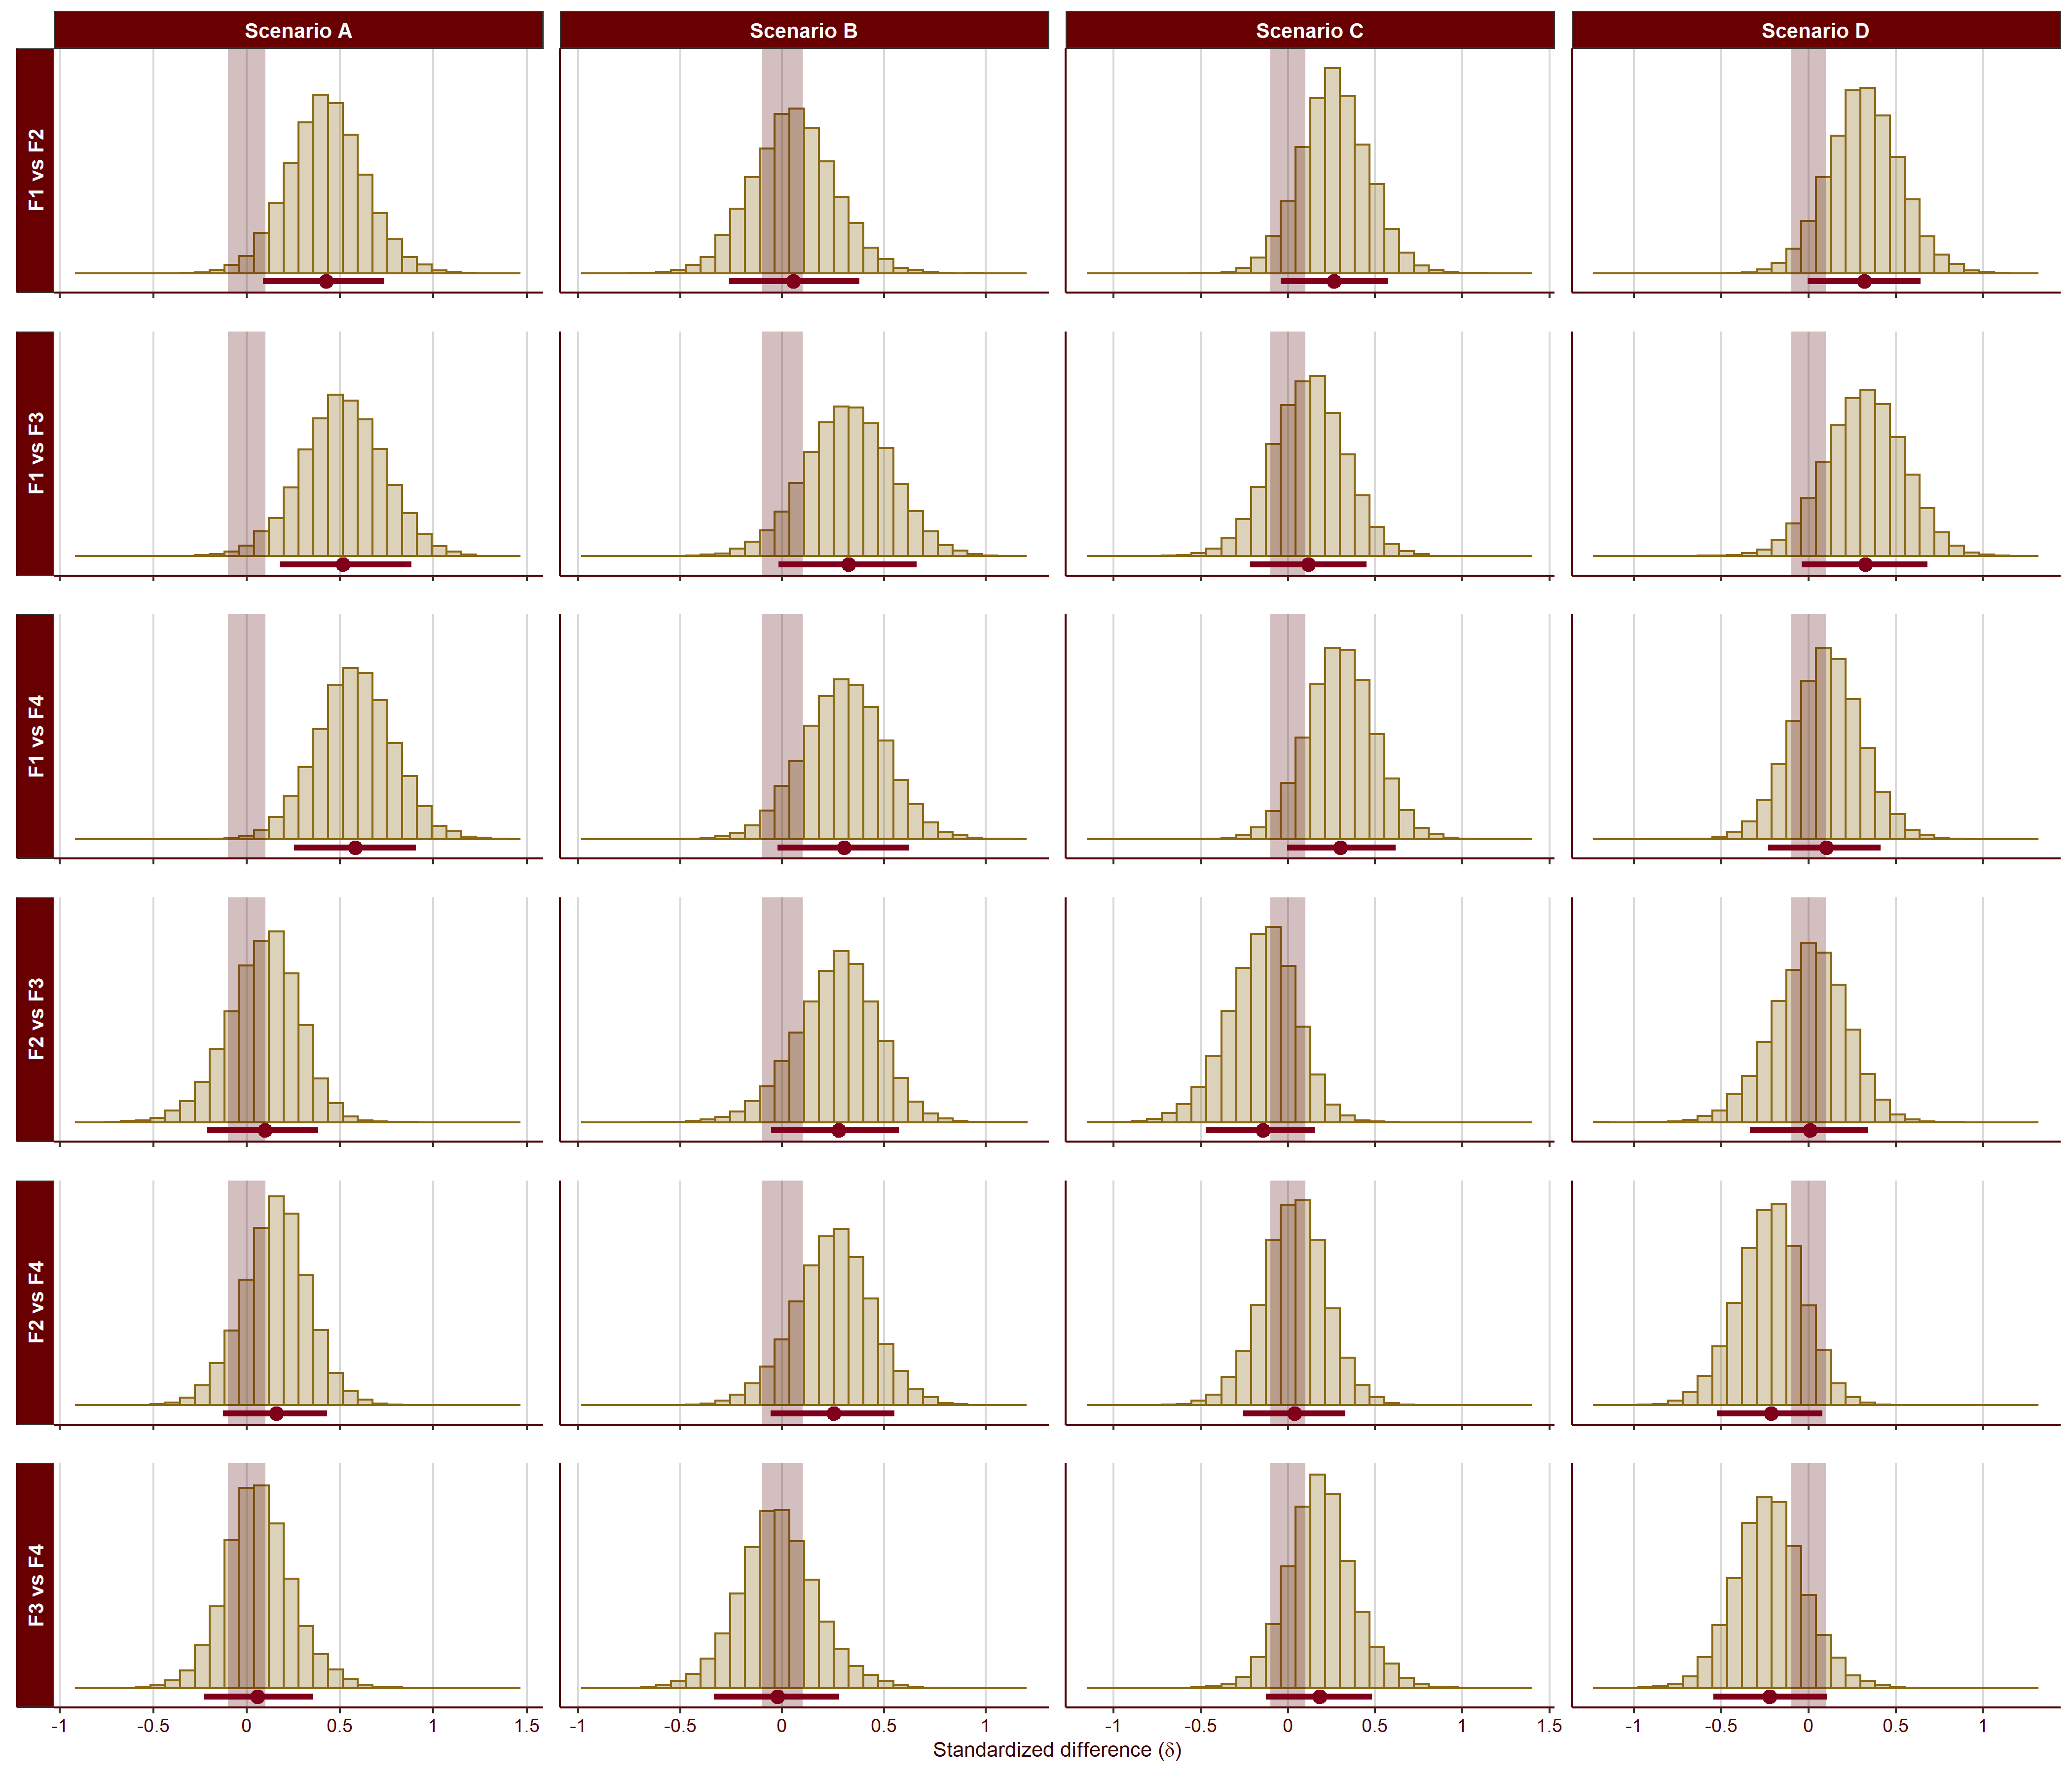
\includegraphics[width=\linewidth]{Figures/SD2_proportion_scenario_comparisons_C.png}
\subcaption{Tallying}
\label{fig:proportion-scenario-comparisons-C}
\end{subfigure}
\caption[]{Continued}
\end{figure}

\medskip

\begin{figure}[ht]\ContinuedFloat
\centering
\begin{subfigure}{1\textwidth}
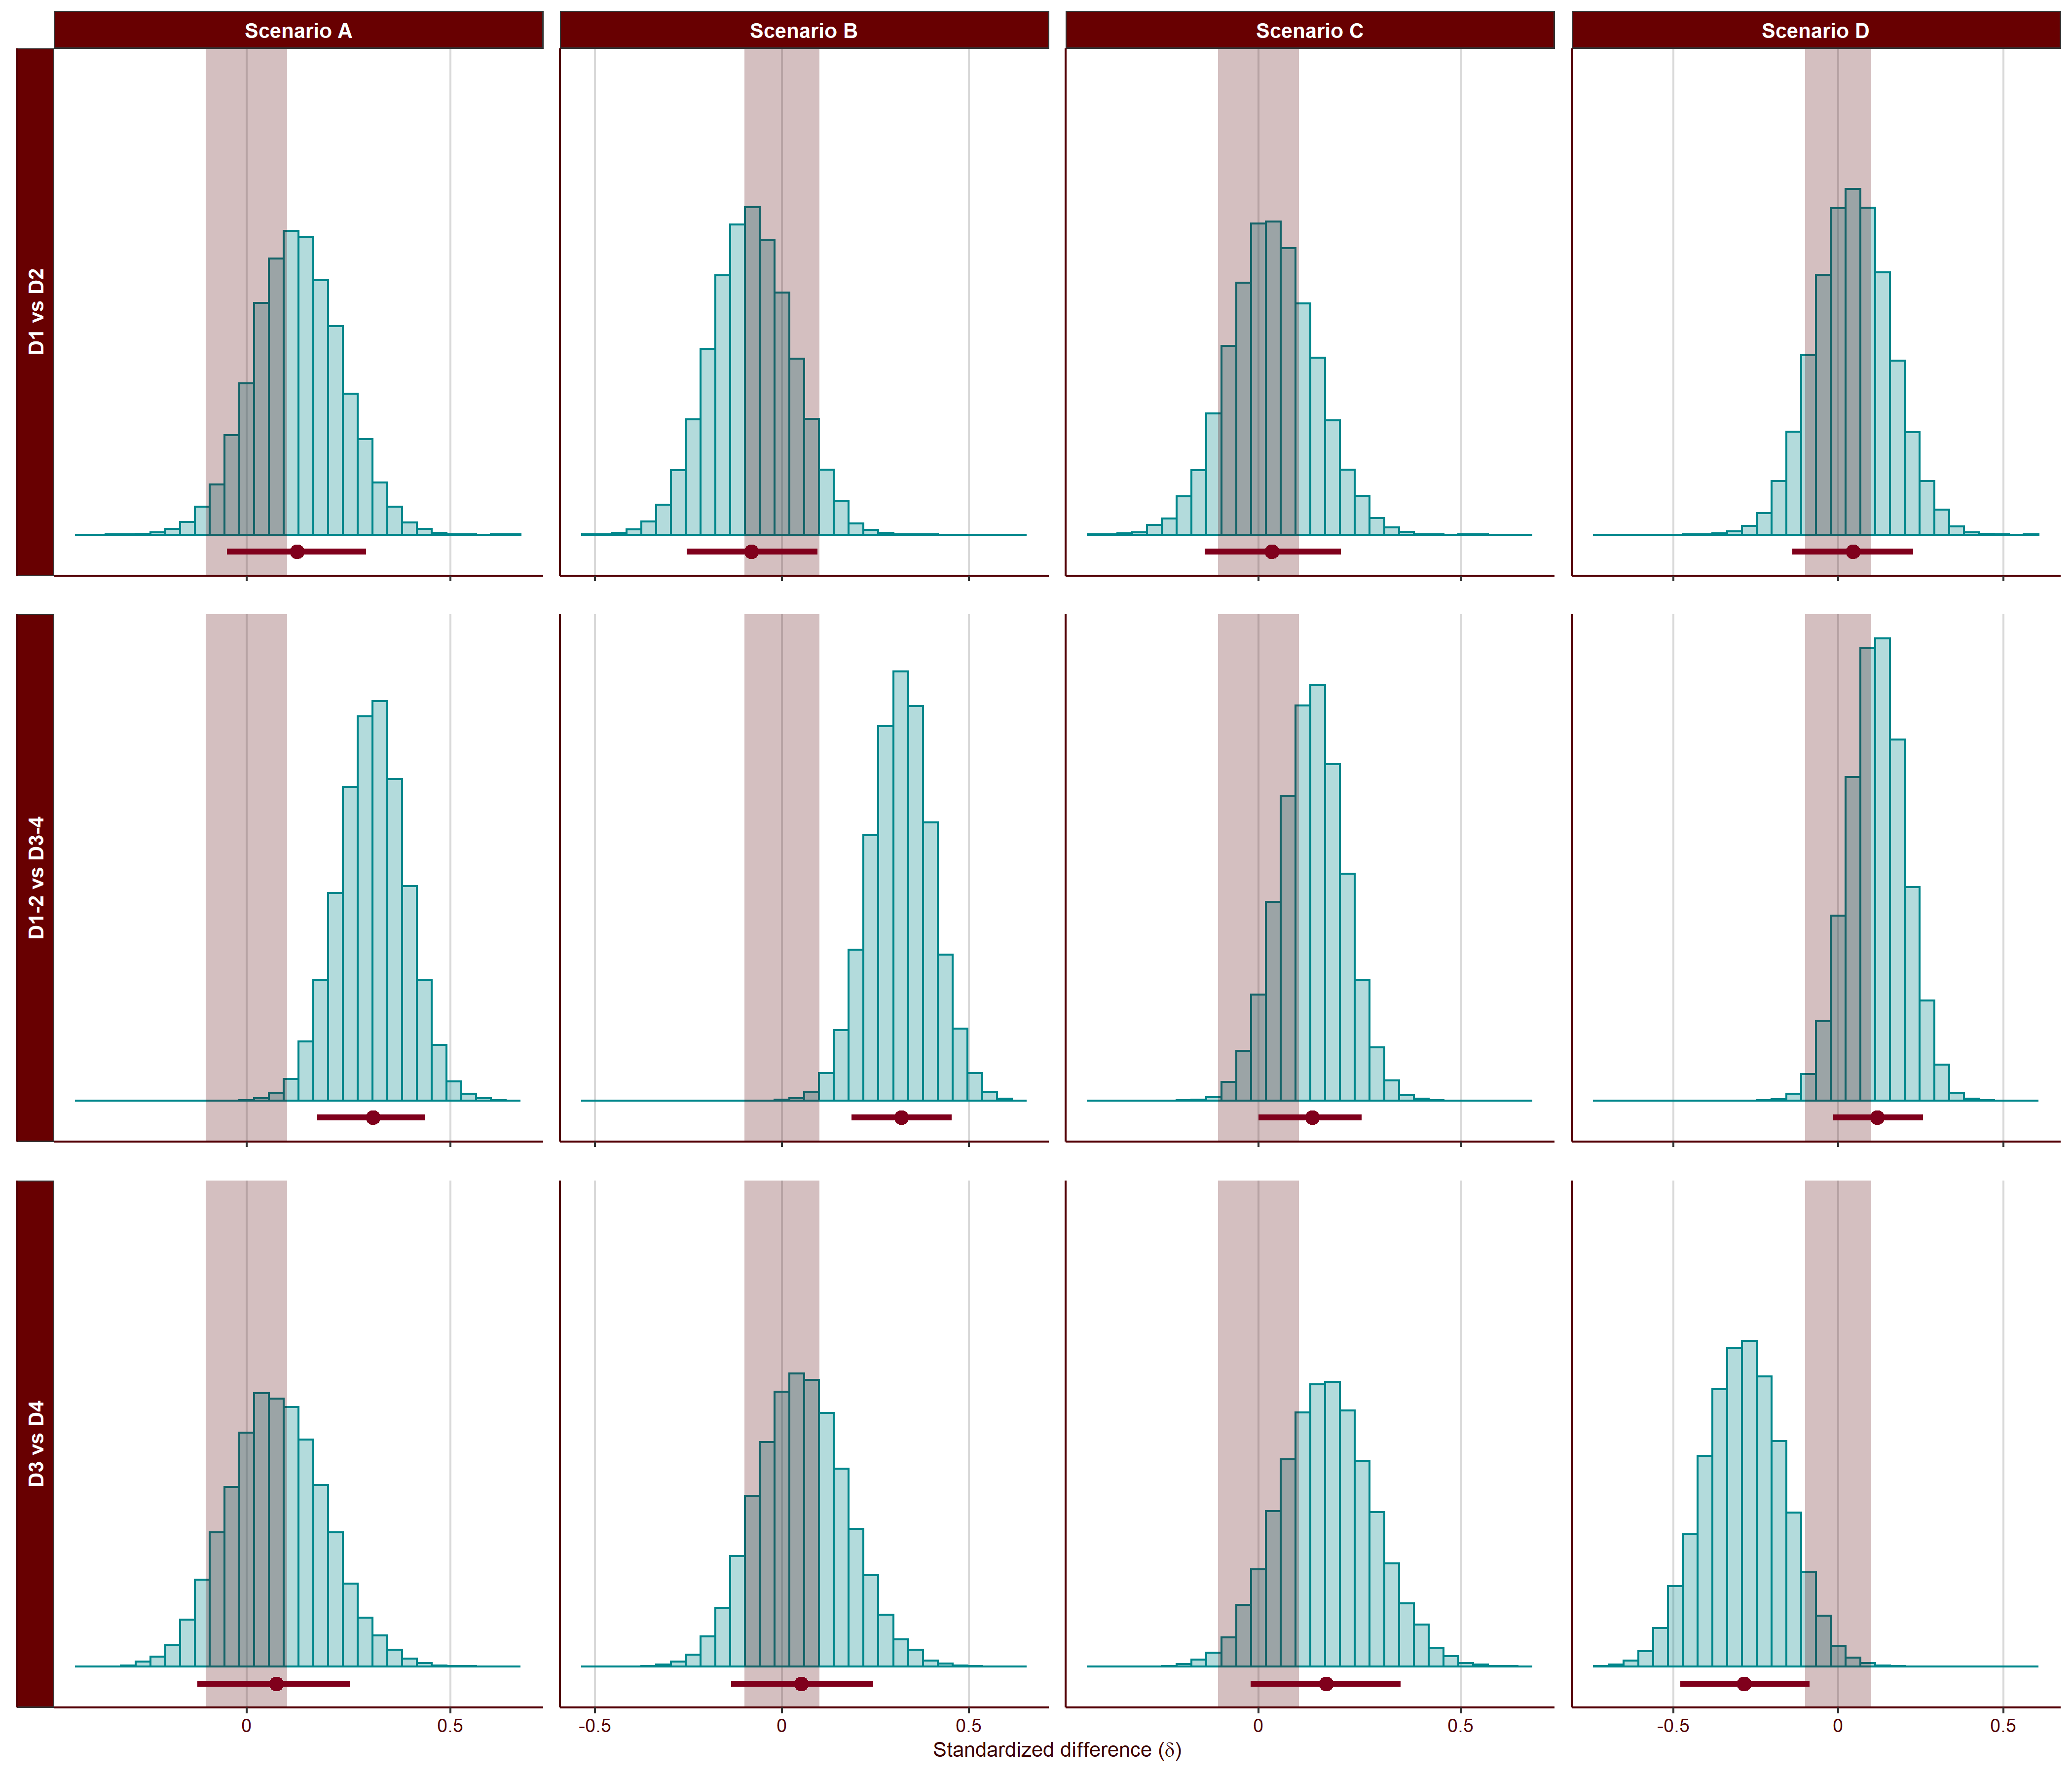
\includegraphics[width=\linewidth]{Figures/SD2_proportion_scenario_comparisons_D.png}
\subcaption{Partial Tallying}
\label{fig:proportion-scenario-comparisons-D}
\end{subfigure}
\caption[]{Continued}
\label{fig:proportion-scenario-comparisons}
\end{figure}

\begin{figure}[!b]
\centering
\begin{subfigure}{1\textwidth}
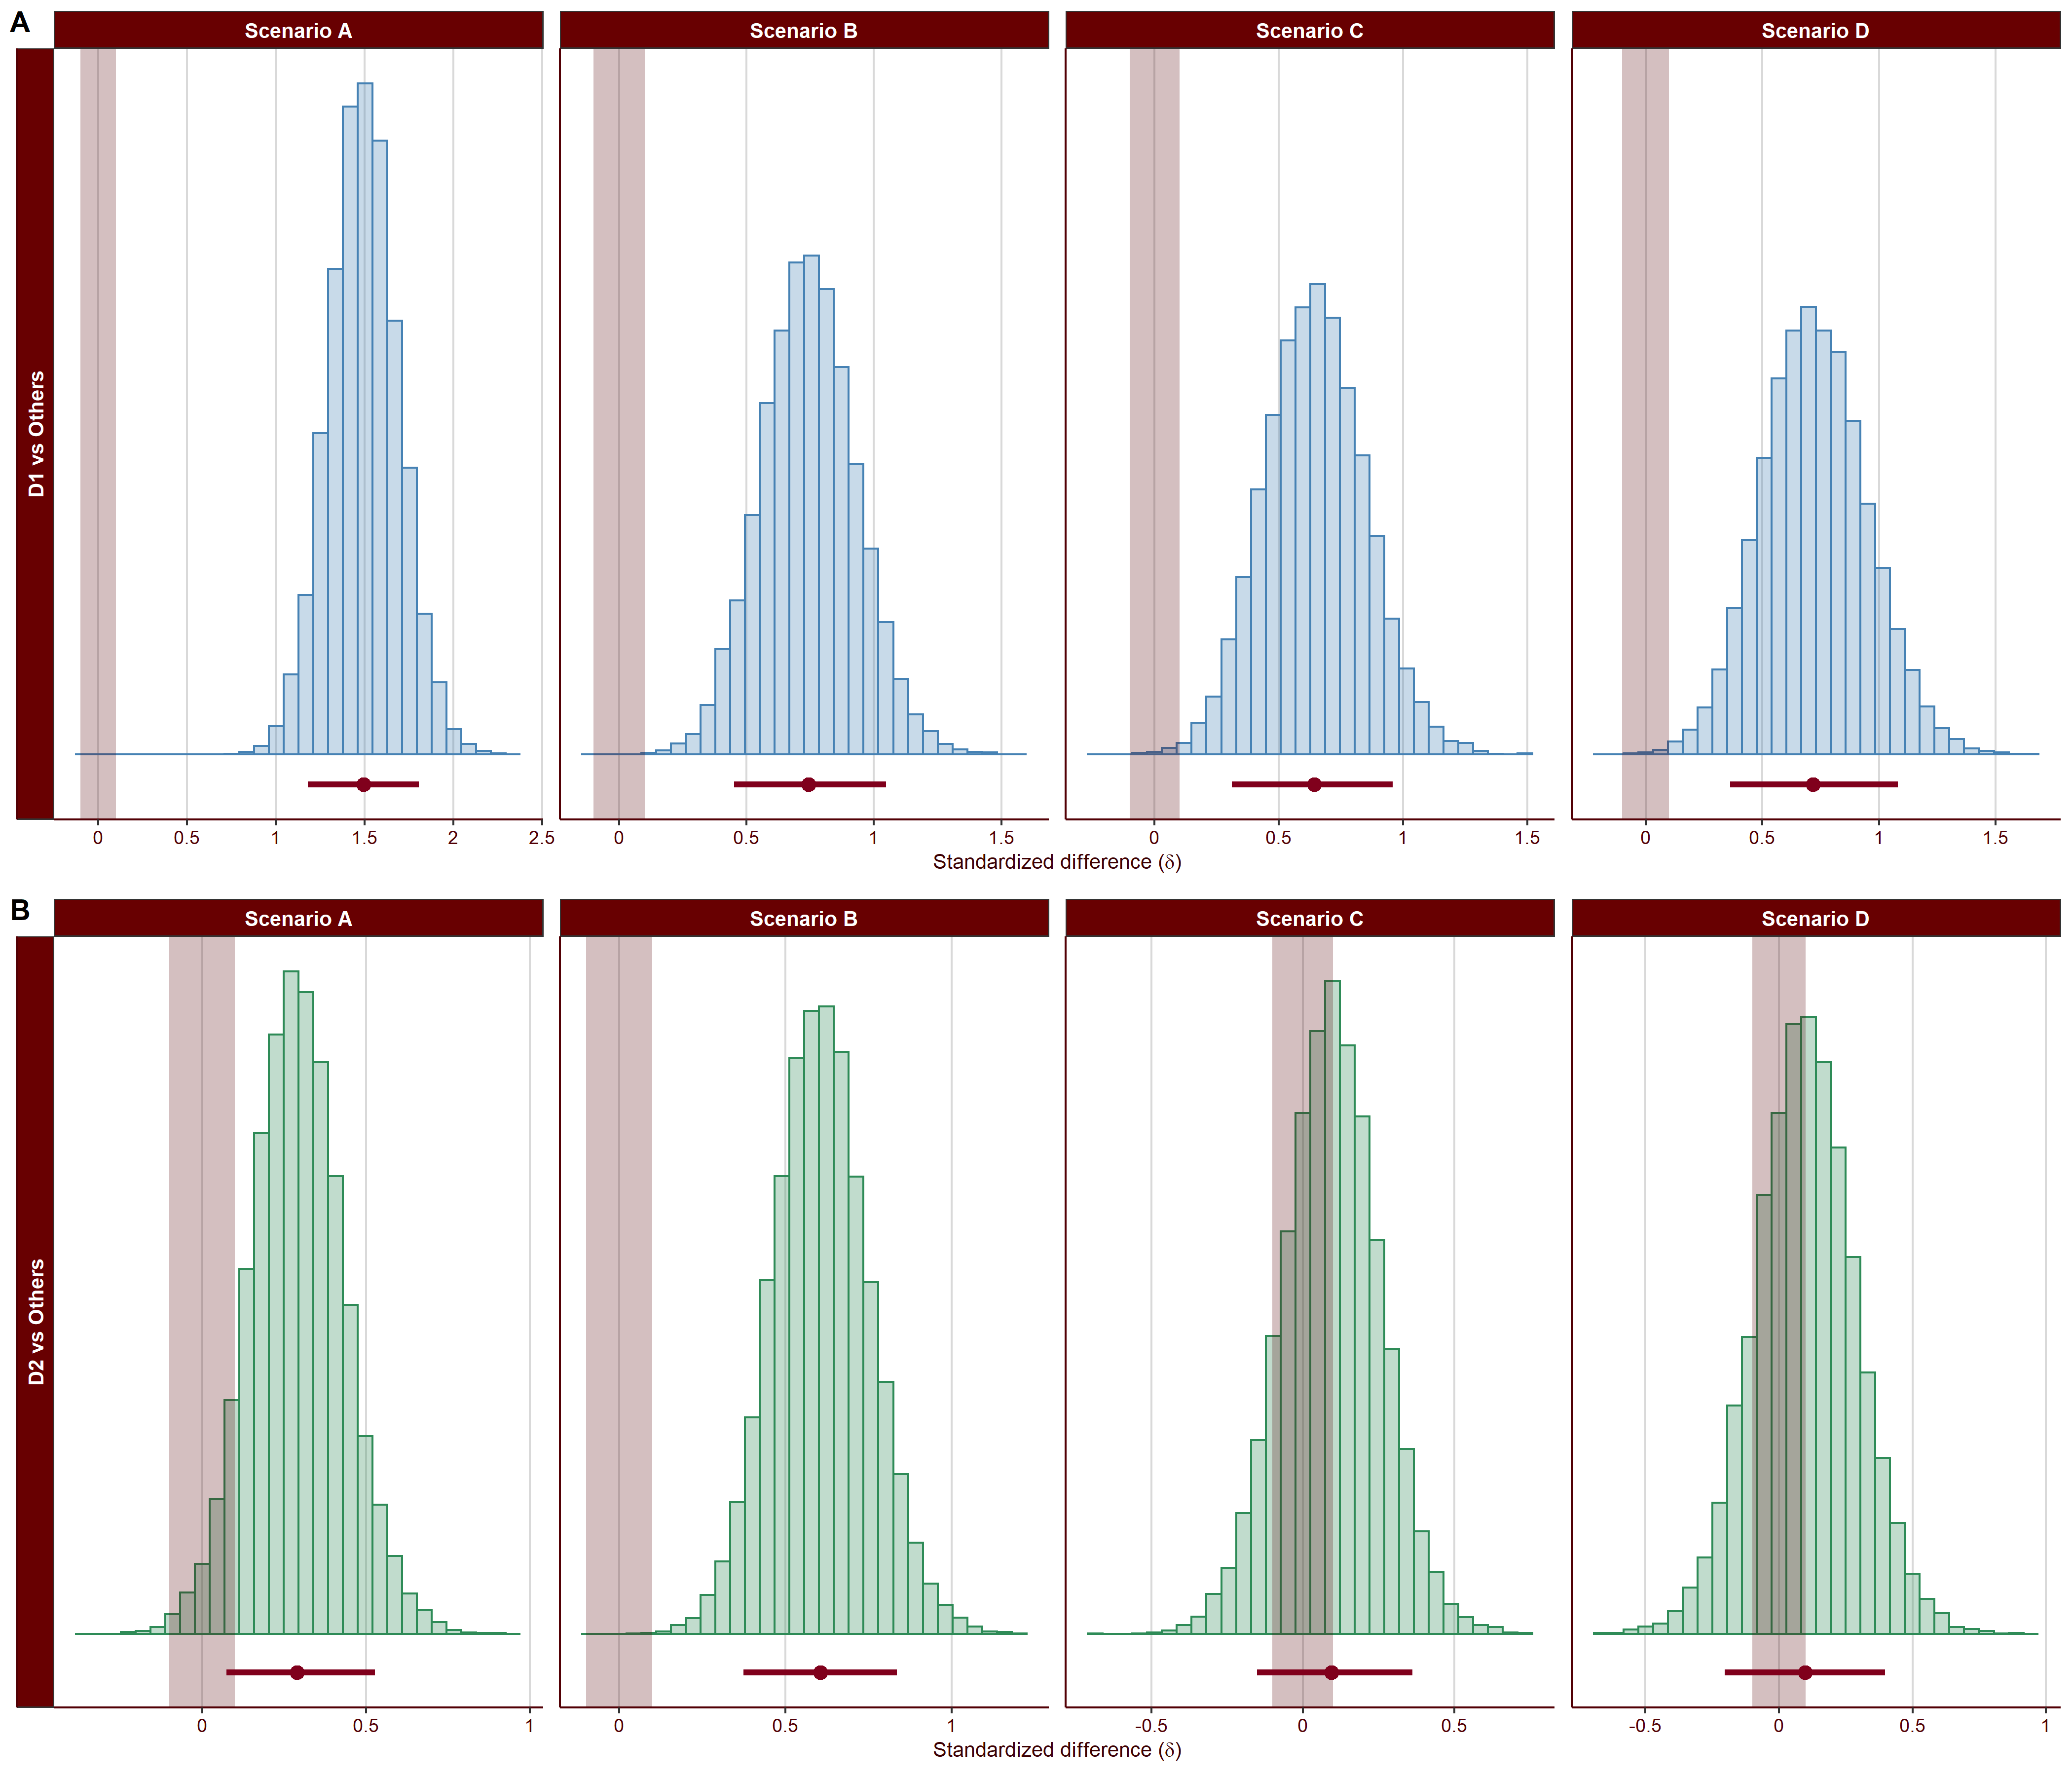
\includegraphics[width=\linewidth]{Figures/SE2_last_scenario_comparisons_A.png}
\subcaption{1st only (A), 2nd only (B)}
\label{fig:last-scenario-comparisons-A}
\end{subfigure}
\caption[]{Follow up comparisons for the allocation of last fixations across decision groups in the different decision scenarios. The horizontal red bar represents the 0.89 HDI. The shaded area highlights the ROPE used in these comparisons}
\end{figure}

\medskip

\begin{figure}[ht]\ContinuedFloat
\centering
\begin{subfigure}{1\textwidth}
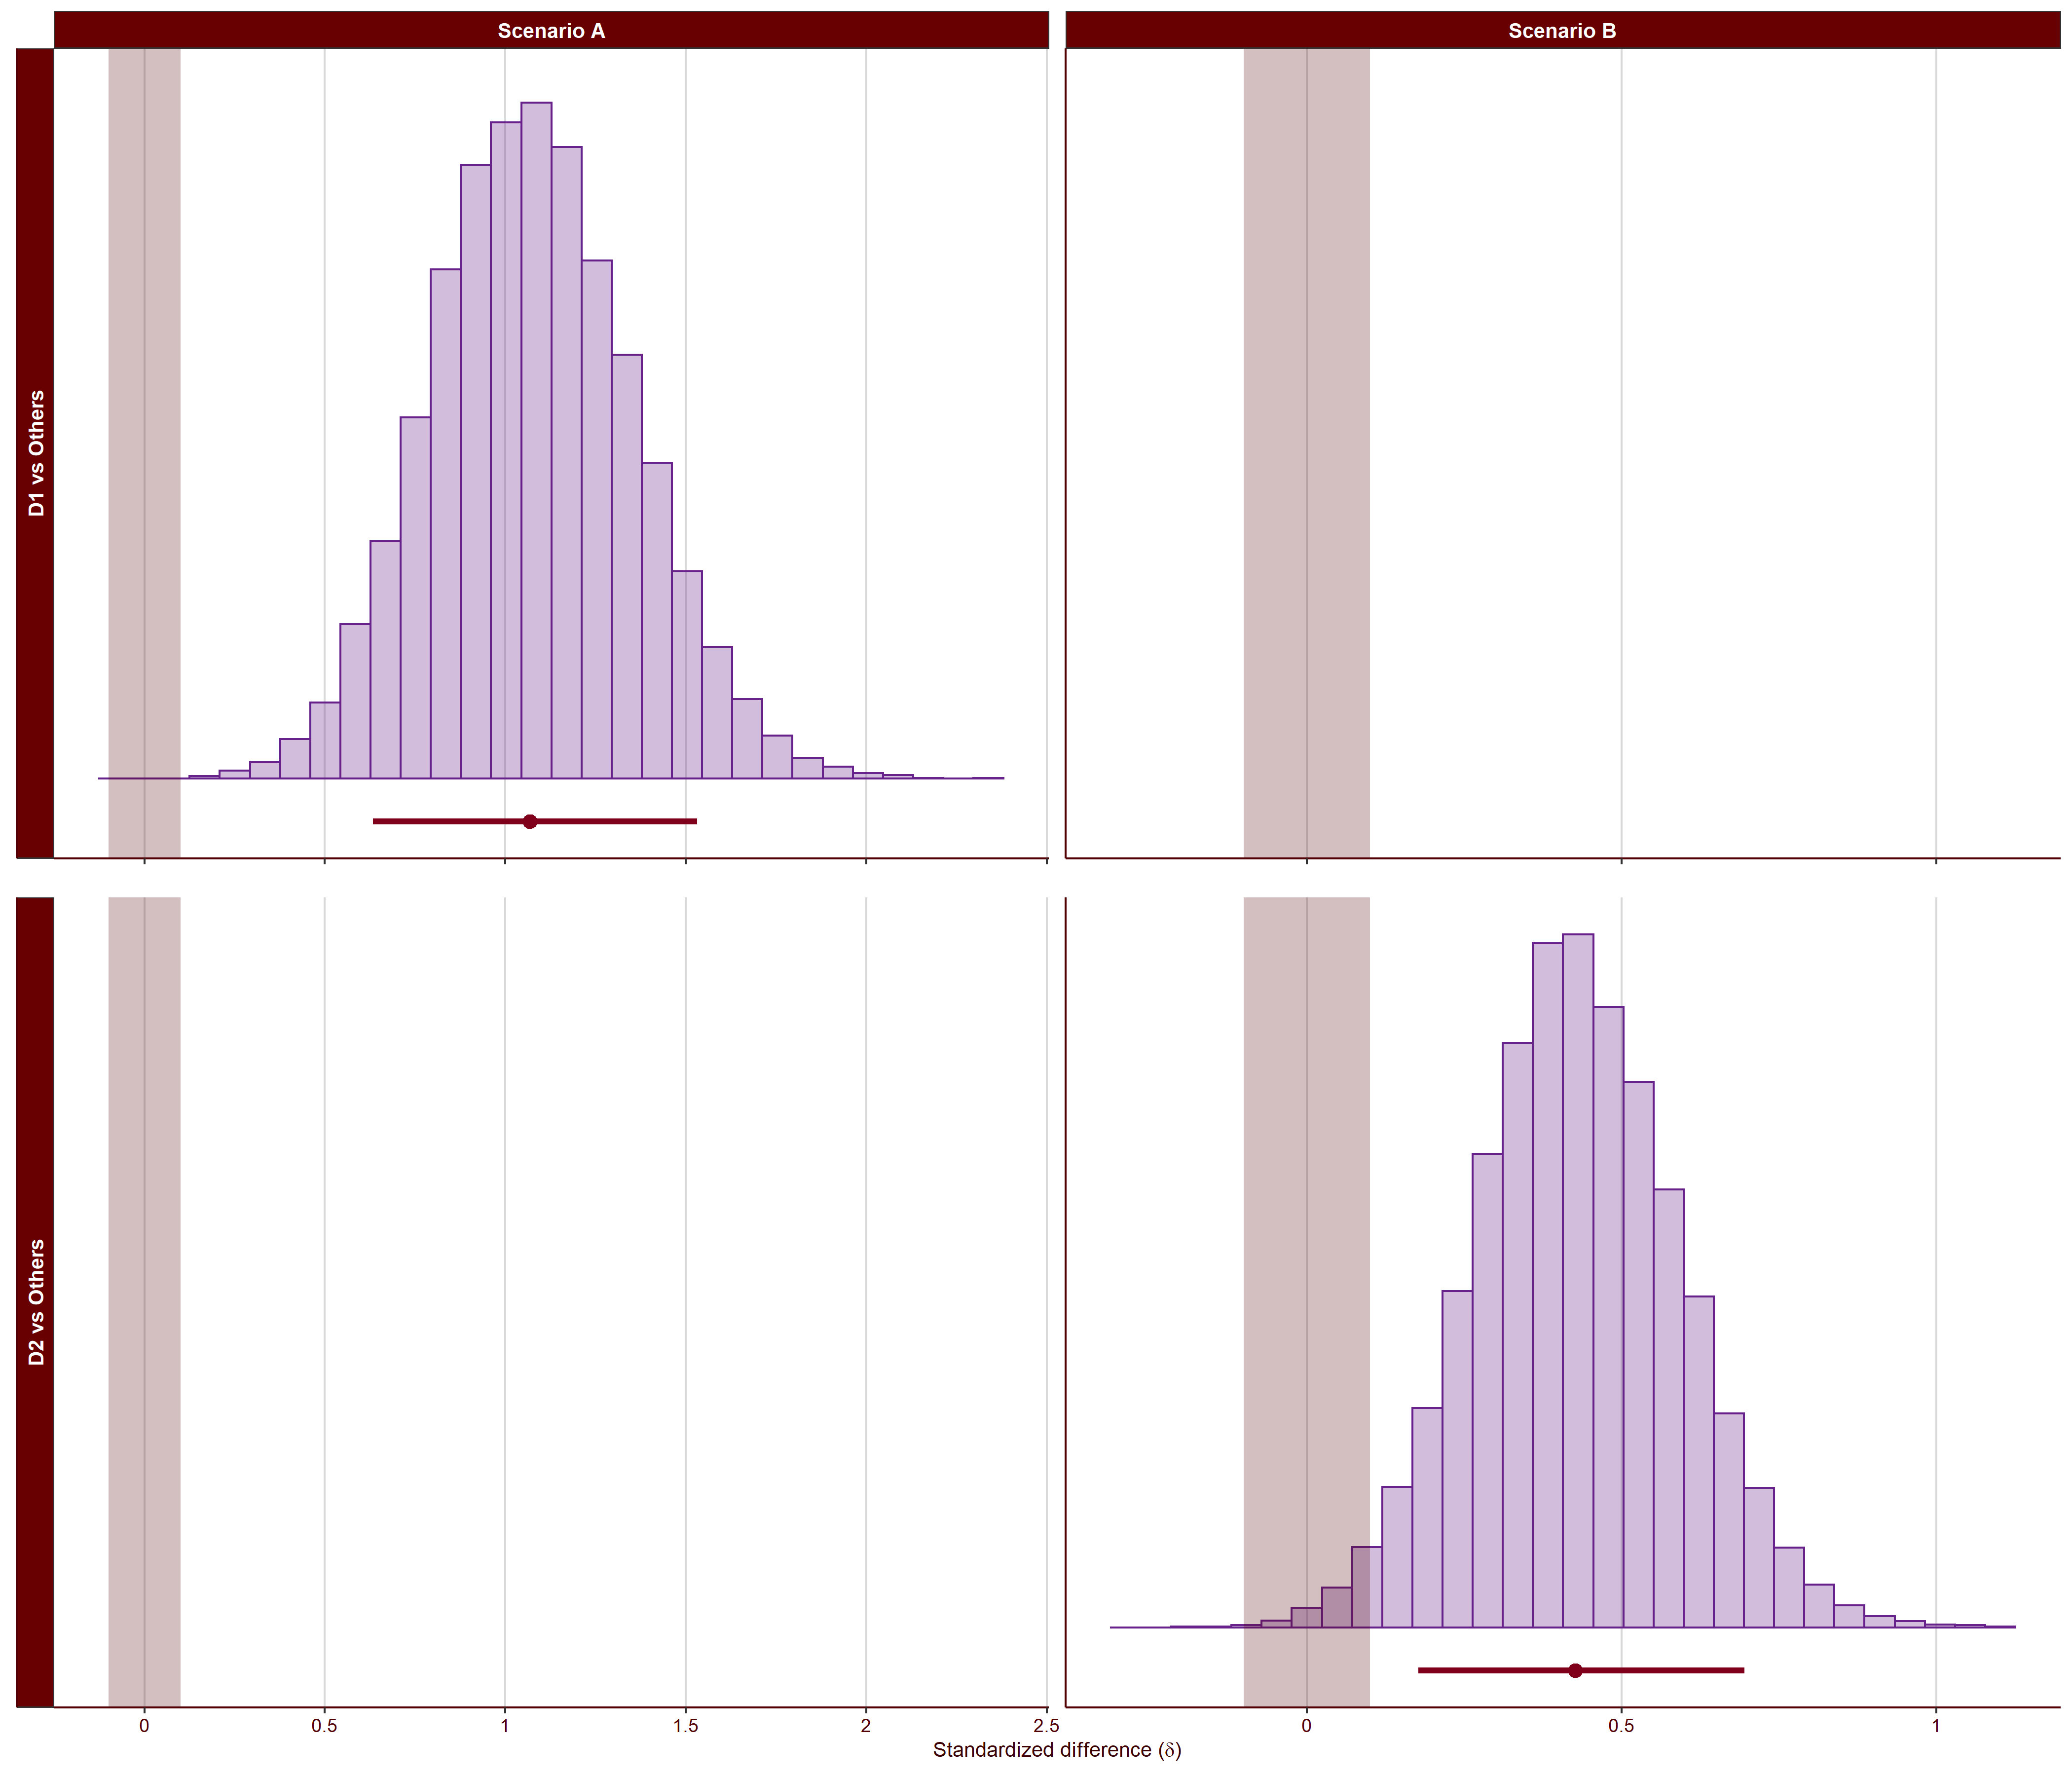
\includegraphics[width=\linewidth]{Figures/SE2_last_scenario_comparisons_B.png}
\subcaption{Serial Search}
\label{fig:last-scenario-comparisons-B}
\end{subfigure}
\caption[]{Continued}
\end{figure}

\medskip

\begin{figure}[ht]\ContinuedFloat
\centering
\begin{subfigure}{1\textwidth}
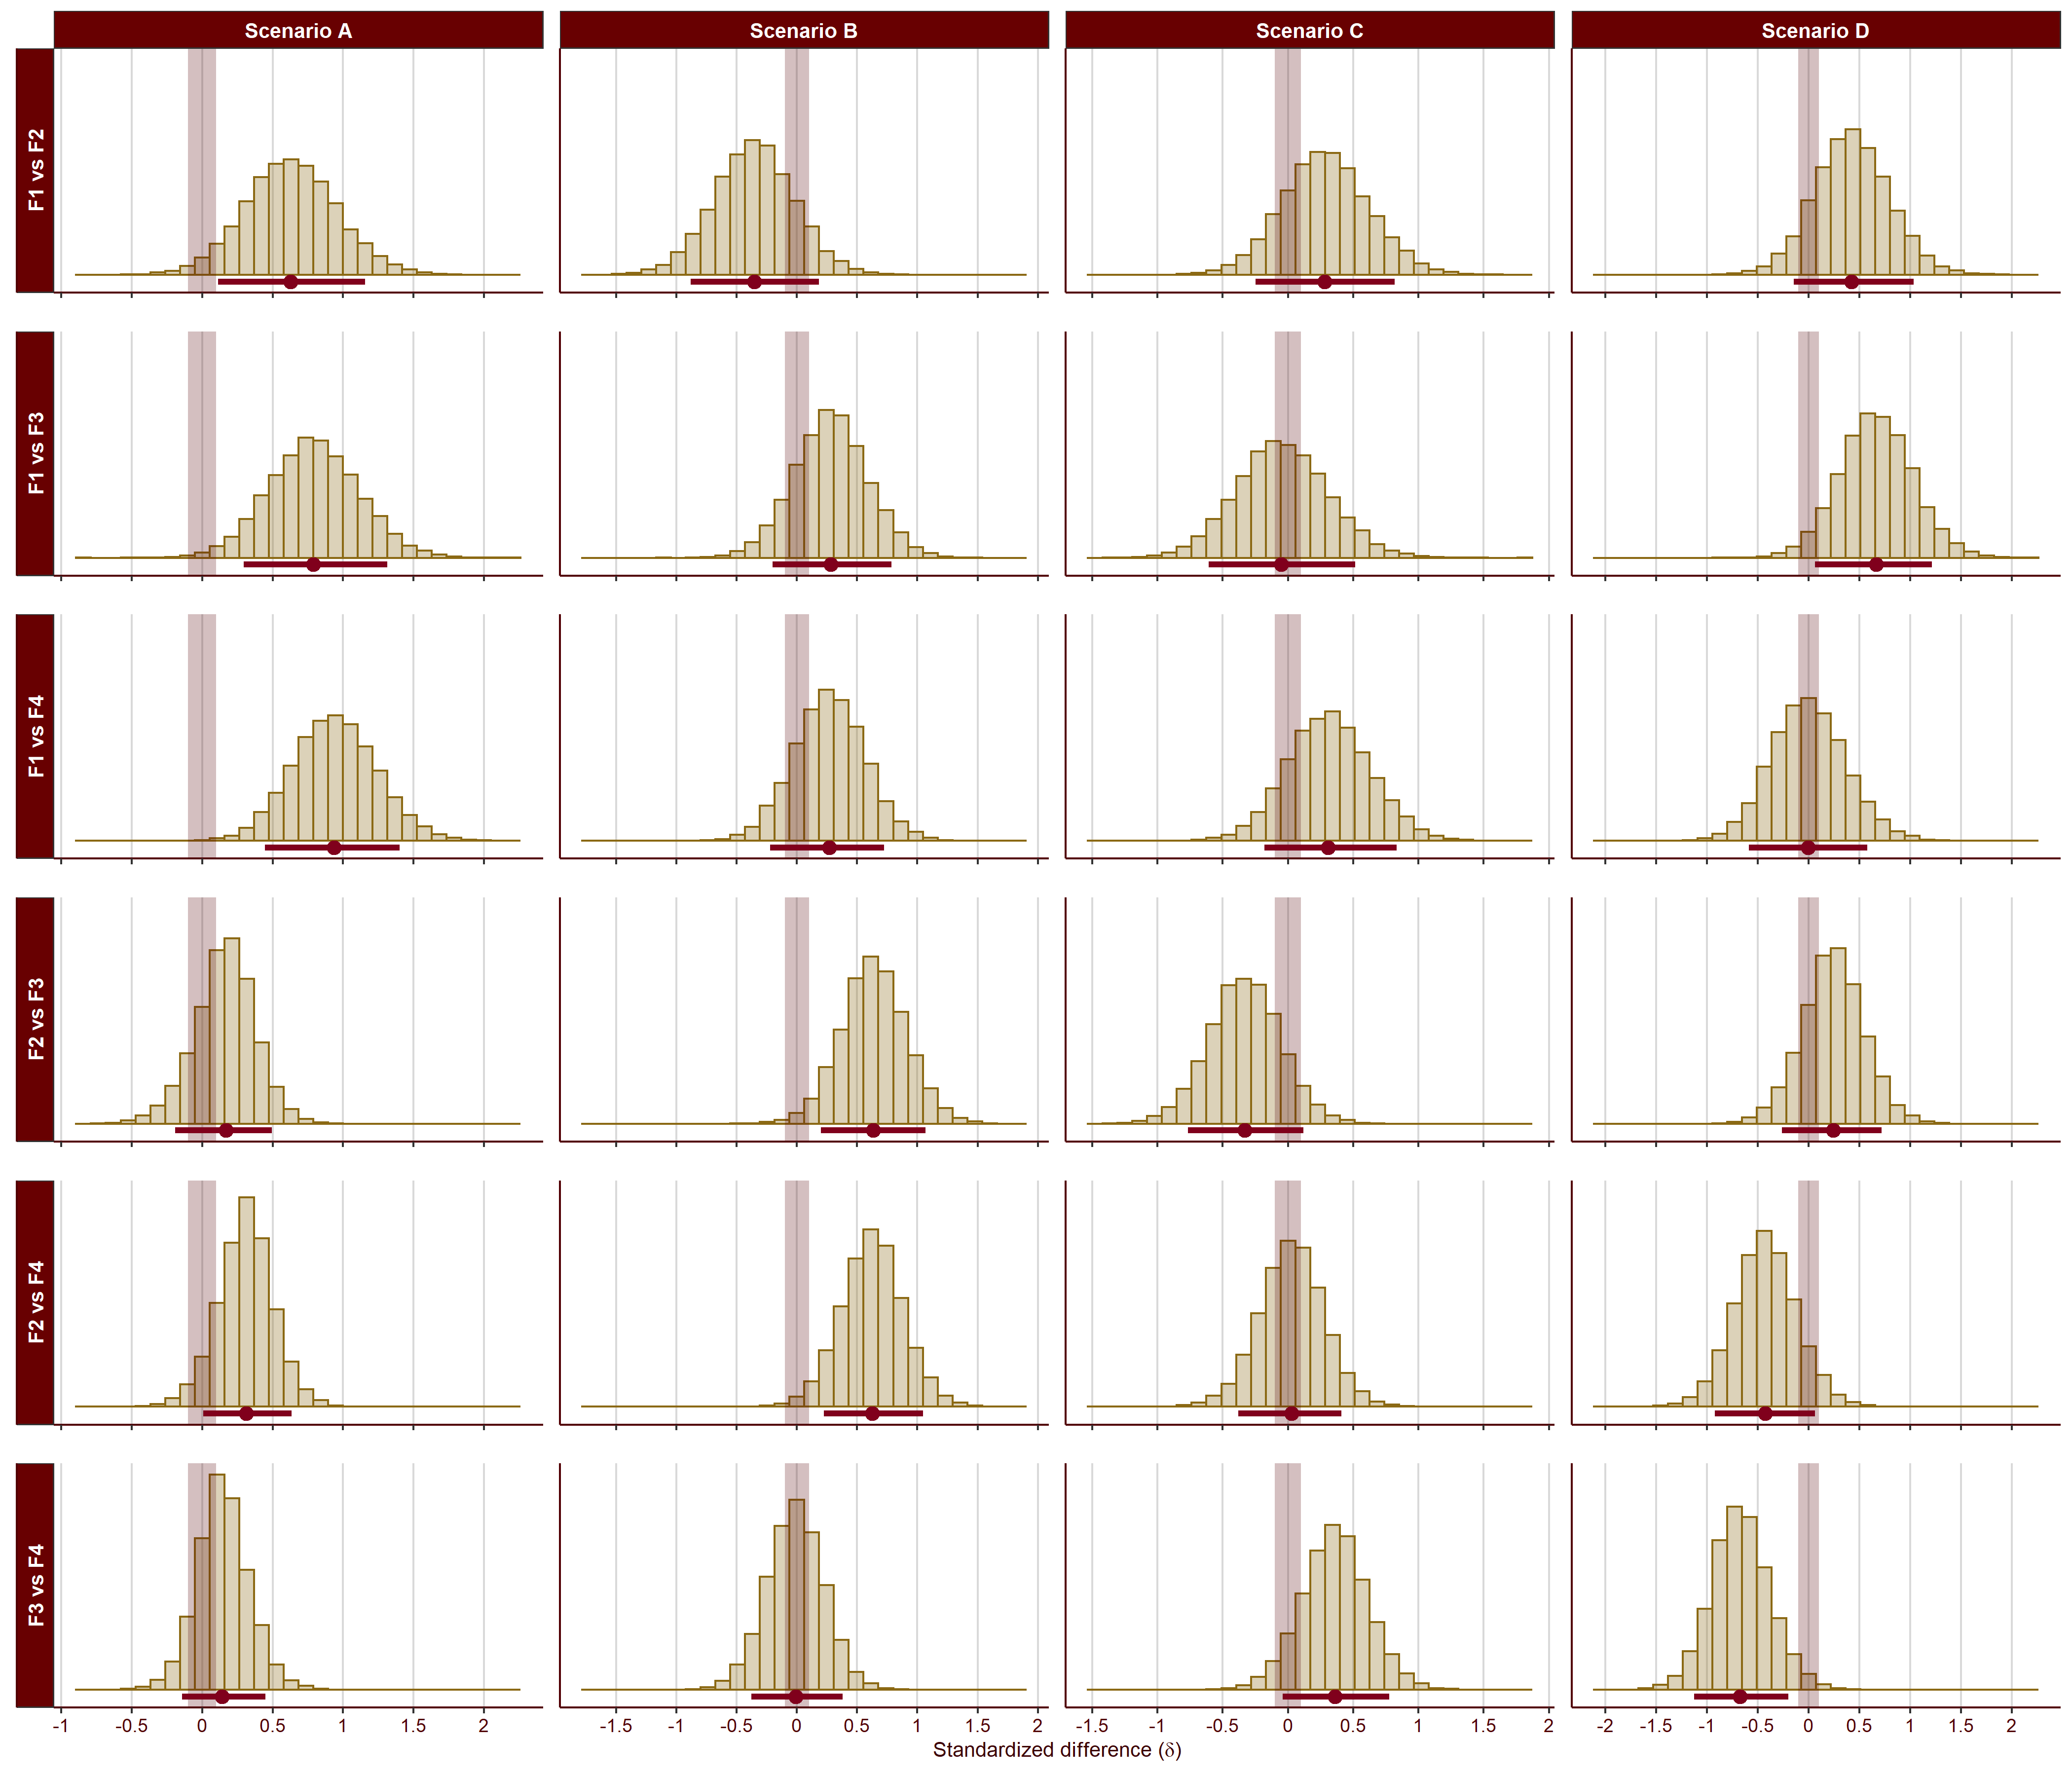
\includegraphics[width=\linewidth]{Figures/SE2_last_scenario_comparisons_C.png}
\subcaption{Tallying}
\label{fig:last-scenario-comparisons-C}
\end{subfigure}
\caption[]{Continued}
\end{figure}

\medskip

\begin{figure}[ht]\ContinuedFloat
\centering
\begin{subfigure}{1\textwidth}
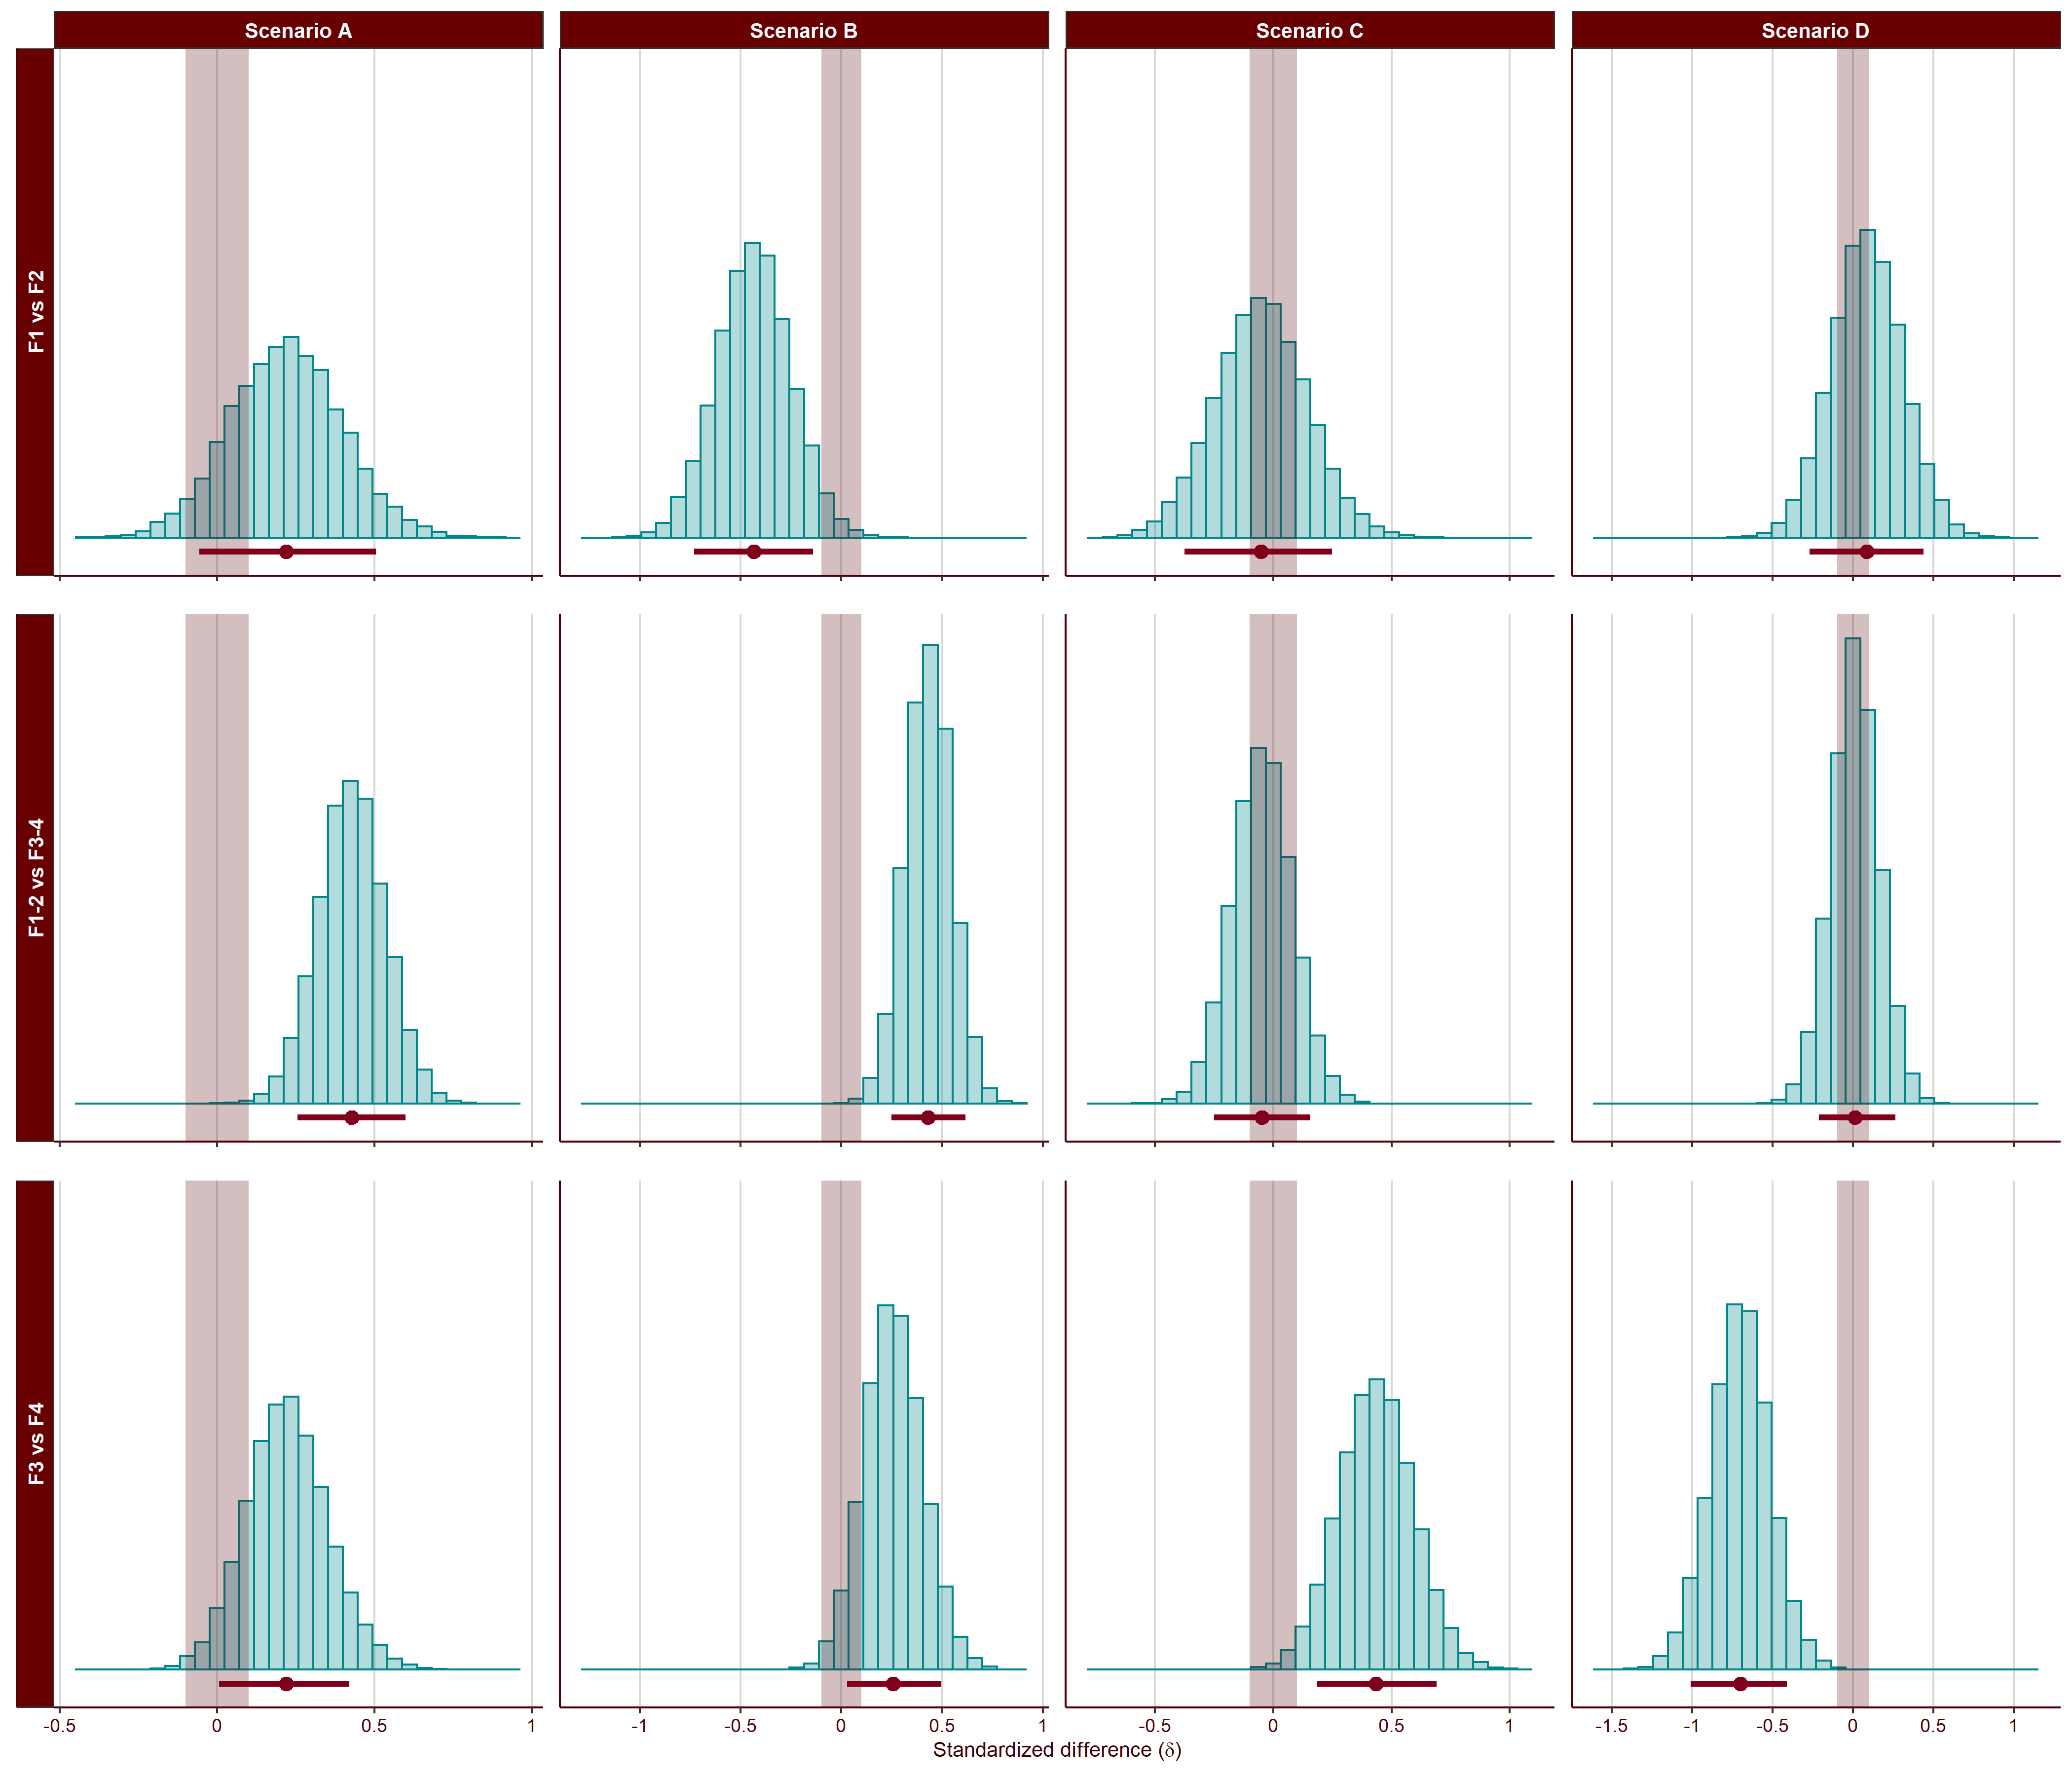
\includegraphics[width=\linewidth]{Figures/SE2_last_scenario_comparisons_D.png}
\subcaption{Partial Tallying}
\label{fig:last-scenario-comparisons-D}
\end{subfigure}
\caption[]{Continued}
\label{fig:last-scenario-comparisons}
\end{figure}
\end{appendix}

\end{document}
